\documentclass[ngerman,11pt,twoside]{scrbook}
\usepackage[breaklinks,colorlinks=true,citecolor=blue,linkcolor=blue,urlcolor=blue,filecolor=blue]{hyperref}
\usepackage{helvet}
\renewcommand{\familydefault}{\sfdefault}
\usepackage{graphicx,color}
\usepackage{url}
\usepackage[utf8]{inputenc}
\usepackage{verbatim}
\usepackage{caption}
\usepackage{latexsym}
\usepackage{setspace}
\usepackage{microtype}
\usepackage{tabularx}
\usepackage{enumitem}
\usepackage{underscore}
\usepackage[automark]{scrlayer-scrpage}
\usepackage[ngerman]{babel}
\usepackage{blindtext}

\raggedbottom

\onehalfspacing 

% Kopf- und Fußzeile
\cleardoublepage
\clearpairofpagestyles
\ofoot[\pagemark]{\pagemark}
\pagestyle{scrheadings}

% Seitendefinitionen

\setlength{\topmargin}{1.5cm}
\setlength{\headheight}{12pt}
\setlength{\headsep}{20pt}
\setlength{\topskip}{12pt}
\setlength{\evensidemargin}{11pt}
\setlength{\oddsidemargin}{-11pt}
\setlength{\textheight}{240mm}
\setlength{\textwidth}{160mm}
\setlength{\voffset}{-2cm}
\setlength{\parindent}{0pt}
\setlength{\parskip}{6pt}

% Code
\usepackage{listings}
\usepackage{xcolor}

\renewcommand{\lstlistingname}{Quellcode}
\definecolor{codegreen}{rgb}{0,0.6,0}
\definecolor{codegray}{rgb}{0.5,0.5,0.5}
\definecolor{codepurple}{rgb}{0.58,0,0.82}
\definecolor{backcolour}{rgb}{0.95,0.95,0.92}

\lstdefinestyle{mystyle}{
	language=Java, 
    backgroundcolor=\color{backcolour},   
    commentstyle=\color{codegreen},
    keywordstyle=\color{magenta},
    numberstyle=\tiny\color{codegray},
    stringstyle=\color{codepurple},
    basicstyle=\ttfamily\footnotesize,
    breakatwhitespace=false,         
    breaklines=true,                 
    captionpos=b,                    
    keepspaces=true,                 
    numbers=left,                    
    numbersep=5pt,                  
    showspaces=false,                
    showstringspaces=false,
    showtabs=false,                  
    tabsize=2
}

\lstset{style=mystyle}


\newcommand{\saauthor}{Patrik Löffler}
\newcommand{\matrikel}{56207}
\newcommand{\sathema}{Modellgetriebene Entwicklung von Microservices}

\newcommand{\saprof}{Prof. Dr.-Ing. habil. Armin Zimmermann}
\newcommand{\sabetreuer}{Dipl.-Inf. Tino Jungebloud}
\newcommand{\invnr}{}


%%%%%%%%%%%%%%%%%%%%%%%%%%%%%%%%%%%%%%%%%%%%%%%%%%%%%%%%%%%%%%%%%
\begin{document}
\begin{titlepage}

\begin{center}

\includegraphics[height=5cm]{bilder/logo.png}

Institut für Technische Informatik und Ingenieurinformatik \\
Fakultät für Informatik und Automatisierung\\
Fachgebiet System- und Software-Engineering

\vspace{3cm}

{\Large Bachelorarbeit} \\ 
\vspace{1cm}
{\huge \normalfont \bfseries \sathema} \\
\vspace{1cm}
{vorgelegt von} \\
\vspace{0.5cm}
{\large \saauthor}\\
{\large Matrikelnummer \matrikel}
\vspace{2cm}

Betreuer: \\
\vspace{0.5cm}
\saprof \\
\sabetreuer \\

\vspace{1cm}

Ilmenau, den \today
\end{center}

\end{titlepage}

\newpage

\chapter*{Selbstständigkeitserklärung}
\thispagestyle{empty}	%keine Seitenzahl!
\pdfbookmark{Selbstständigkeitserklärung}{Selbstständigkeitserklärung}

Hiermit erkläre ich, dass ich die vorliegende Arbeit
selbstständig angefertigt, nicht anderweitig zu Prüfungszwecken vorgelegt und
keine anderen als die angegebenen Hilfsmittel verwendet habe. Sämtliche 
wissentlich verwendete Textausschnitte, Zitate oder Inhalte anderer Verfasser 
wurden ausdrücklich als solche gekennzeichnet.\\[2ex]
Ilmenau, den \today\\[6ex]
\newlength\us
\settowidth{\us}{-Patrik~Löffler-}
\begin{tabular}{p{\us}}\hline
\centering\footnotesize Patrik~Löffler
\end{tabular}

\newpage
\cleardoublepage
\thispagestyle{empty}
\vspace*{\fill} 

\begin{center}
\textit{„Ich weiß, dass ich nichts weiß“} \\
\textbf{– Sokrates}
\end{center}

\vspace*{\fill} 

\newpage
\cleardoublepage
\pagenumbering{roman}
\tableofcontents
\newpage
\listoffigures
\newpage

\pagenumbering{arabic}

% Kapitel

\chapter{Abstract}

Diese Arbeit erforscht die modellgetriebene Softwareentwicklung von Microservice-Architekturen. Im Fokus steht die Konzeption eines Metamodells für diese. Ziel ist es, lauffähige und in einer Cloud-Infrastruktur ausführbare Anwendungen zu modellieren und zu generieren. Hierbei sollen die Designprinzipien des Domain-Driven Designs angewendet werden. Die zentralen Beiträge dieser Arbeit umfassen die Analyse der Vor- und Nachteile verschiedener Entwurfsentscheidungen sowie die Überprüfung der Ausdrucksfähigkeit des Metamodells mittels konkreter Syntax und Visualisierung. Ein besonderer Schwerpunkt liegt auf der Untersuchung, wie sich mit diesem Modell Anwendungen für reale Problemdomänen abbilden lassen.

Ein wesentliches Ergebnis ist die erfolgreiche Generierung von Java-Spring-Applikationen, womit die grundlegende Machbarkeit bewiesen wird. Weiterhin werden dabei auftretende Probleme und mögliche Lösungsansätze im Kontext der Codegenerierung beleuchtet. Zudem wird erforscht, inwiefern sich dieser modellgetriebene Ansatz für Refaktorisierungen einsetzen lässt. Theoretische Grundlagen und eine umfassende State-of-the-Art-Recherche bilden das Fundament dieser Arbeit. Methodisch wurde ein schichtbasiertes Konzept für die Abstraktion entwickelt, das iterativ verfeinert und durch anwendungsfokussierte Entwurfsentscheidungen ergänzt wurde.

Neben der Realisierbarkeit der Metamodellierung verschiedener Aspekte von Microservice-Architekturen konnte auch die variierende Komplexität der einzelnen Aspekte und Ansätze zu deren Lösung aufgezeigt werden. Darüber hinaus werfen die Herausforderungen und Grenzen des aktuellen Ansatzes neue Fragestellungen auf. Insbesondere wird diskutiert, inwiefern eine vertiefende Modellierung dieser Domäne, ergänzend zur breiten Perspektive, nützlich sein könnte. Diese Erkenntnisse bieten wichtige Impulse für zukünftige Forschungen in der modellgetriebenen Entwicklung von Microservices.

\newpage

This work explores the model-driven software development of microservice architectures. The focus is on the conception of a metamodel for these. The goal is to model and generate applications that are runnable and executable in a cloud infrastructure. In this process, the design principles of Domain-Driven Design are to be applied. The central contributions of this work include the analysis of the advantages and disadvantages of various design decisions, as well as the examination of the expressiveness of the metamodel through concrete syntax and visualization. A particular emphasis is placed on investigating how this model can represent applications for real problem domains.

A key result is the successful generation of Java-Spring applications, proving the fundamental feasibility. Furthermore, problems that arise and potential solutions in the context of code generation are illuminated. Additionally, it explores to what extent this model-driven approach can be used for refactorings. Theoretical foundations and a comprehensive state-of-the-art research form the basis of this work. Methodologically, a layer-based concept for abstraction was developed, which was iteratively refined and supplemented by application-focused design decisions.

Besides the realizability of the metamodeling of various aspects of microservice architectures, the varying complexity of the individual aspects and approaches to their solutions was also demonstrated. Moreover, the challenges and limitations of the current approach raise new questions. In particular, it discusses to what extent a more in-depth modeling of this domain, in addition to the broad perspective, could be useful. These insights provide important impulses for future research in the model-driven development of microservices.

\newpage

\chapter{Einleitung}

\section{Motivation}

In einer dieser vorangegangenen Seminararbeit wurde bereits aufgezeigt, dass Webdienste mittels modellgetriebener Softwareentwicklung umgesetzt werden können. Auf dieser Grundlage strebt diese Arbeit an, einen verfeinerten Ansatz zu entwickeln, der sich spezifisch auf die Microservice-Architektur von Webdiensten fokussiert. Die Entwicklung von Microservices – kleinen, skalierbaren Anwendungen, die oft in verteilten Systemen Verwendung finden – könnte von Vorteilen wie gesteigerter Wiederverwendbarkeit, vereinfachter Wartung und generell beschleunigter Entwicklungszeit profitieren. Besonders interessant ist dabei das mögliche Potenzial welches im Kontext von abhängigkeitsbezogenen Migrationen im Softwarelebenszyklus existieren könnte. Es stellt sich jedoch die Frage, ob Microservice-Anwendungen in ihrer gesamten konzeptionellen Breite durch ein Metamodell adäquat erfasst werden können. Zudem sind die domänenspezifischen Herausforderungen, die sich hierbei ergeben, von besonderem Interesse \cite{loeffler}.

\section{Zielstellung}

Ziel der Arbeit ist es, Anwendungen, die das Microservice-Paradigma verwenden, mit Werkzeugen und Methoden der modellgetriebenen Softwareentwicklung zu entwickeln. Dazu wird eine Domänenspezifische Sprache in Form eines Metamodell konzipiert, welches die grundlegenden Eigenschaften des Paradigmas abstrahiert. Dies wird ergänzt durch die Berücksichtigung von Konzepten des Domain-Driven Design zur Modellierung der Geschäftslogik.

Anwendungen, die mit diesem Metamodell entwickelt werden, sollen Abhängigkeiten, wie Frameworks und Bibliotheken, integrieren. Weiterhin soll untersucht werden, wie diese Anwendungen effektiv migriert werden können. Dabei soll erforscht werden, ob sich ein modellgetriebener Ansatz für die Durchführung von Refaktorisierungen eignet, insbesondere im Kontext von Versionsaktualisierungen bei Abhängigkeiten.

Außerdem wird untersucht, inwiefern die der Anwendung zugrundeliegende IT-Infrastruktur in einem solchen Metamodell berücksichtigt werden kann und ob es möglich ist, Deployment-fähige Anwendungen mithilfe eines Metamodells zu generieren.
\chapter{Grundlagen}

%%%%%%%%%%%%%%%%%%%%%%%%%%%%%%%%%%%%%%%%%%%%%%%%%%%%%%%%%%%%%%%%%%%%%%%%%%%%%%%%%%%%%%%%%%%%%%%%%%%%%%%%%%%%%%%
%
%						DOMAIN	DRIVEN	DESIGN
%
%%%%%%%%%%%%%%%%%%%%%%%%%%%%%%%%%%%%%%%%%%%%%%%%%%%%%%%%%%%%%%%%%%%%%%%%%%%%%%%%%%%%%%%%%%%%%%%%%%%%%%%%%%%%%%%

\section{Domain-Driven Design}

\subsection{Definition}

Die Domäne einer Software bezeichnet das Themengebiet oder den Anwendungsbereich, in dem das Programm eingesetzt wird \cite[S.2]{evans} \cite[S.307]{posch}. \glqq Domain-Driven Design\grqq{} (Abk.: DDD) ist eine Herangehensweise, Problemdomänen in ein Modell für die Softwareentwicklung zu überführen. Modellieren ist eine grundlegende Methode der Wissenschaft um mit komplexen Systemen umzugehen. Eine Abstraktion eines solchen Systems, die es ermöglicht, Fragestellungen dazu zu beantworten, wird als Modell bezeichnet \cite{brugge}.

Geprägt wurde das DDD durch Eric Evans in seinem Buch \glqq Domain-Driven Design: Tackling Complexity in the Heart of Software\grqq{} \cite{evans}. Kern des domänengetriebenen Entwurfs ist es, die reale, oft unübersichtliche Fachlichkeit fortschreitend in feiner geschnittene Teilbereiche zu kapseln. Diese sollen möglichst wenige Abhängigkeiten zueinander haben \cite[S.63, 70]{dowalil}. Dieser auf das Domänenmodell fokussierte Ansatz versucht, Kernaspekte einer Anwendung in das Modell zu integrieren, anstatt sie über externe Dienste einzubinden \cite[S.74]{daschner}.

Evans stellt drei Grundeigenschaften fest, welche bei der Wahl eines Modells im DDD zu berücksichtigen sind \cite[S. 3-4]{evans}:
\begin{itemize}
\item Es existiert immer eine Abhängigkeit zwischen Modell und Implementierung.
\item Die Terminologie während der Softwareentwicklung ist eine Implikation des zugrunde liegenden Modells.
\item Nützliches und aufgearbeitetes Wissen kann diesem Modell entnommen werden.
\end{itemize}

Ein weiteres Kernkonzept des DDD ist die \glqq Ubiquitous Language\grqq{}. Sie verbindet Entwickler und Domänen-Experten durch eine auf dem Modell basierende Sprache. Dabei definiert sie eindeutig die verwendeten Begriffe und die ihnen zugeordneten Fachlichkeiten \cite[S. 25-27]{evans}. Ein weiterer Kern ist das \glqq Model-Driven Design\grqq{{} (Abk.: MDD). MDD betont und bezeichnet das notwendige Ineinandergreifen der Konzeption eines Domänenmodells mit dem Entwurf der Anwendungssoftware. Um eine enge Übereinstimmung zwischen Modell und Software sicherzustellen, ist es von Vorteil, innerhalb eines durch Software-Tools unterstützten Modellierungsansatzes zu arbeiten. Objektorientierte Programmiersprachen eignen sich besonders gut, da sich die objekthaften Eigenschaften von Modellen gut abbilden lassen \cite[S. 49-51]{evans}.


\pagebreak 
\subsection{Bausteine des Model-Driven Design}

Das DDD definiert verschiedene Bausteine des MDD \cite[S. 65]{evans}:

\begin{figure}[ht]
\centering
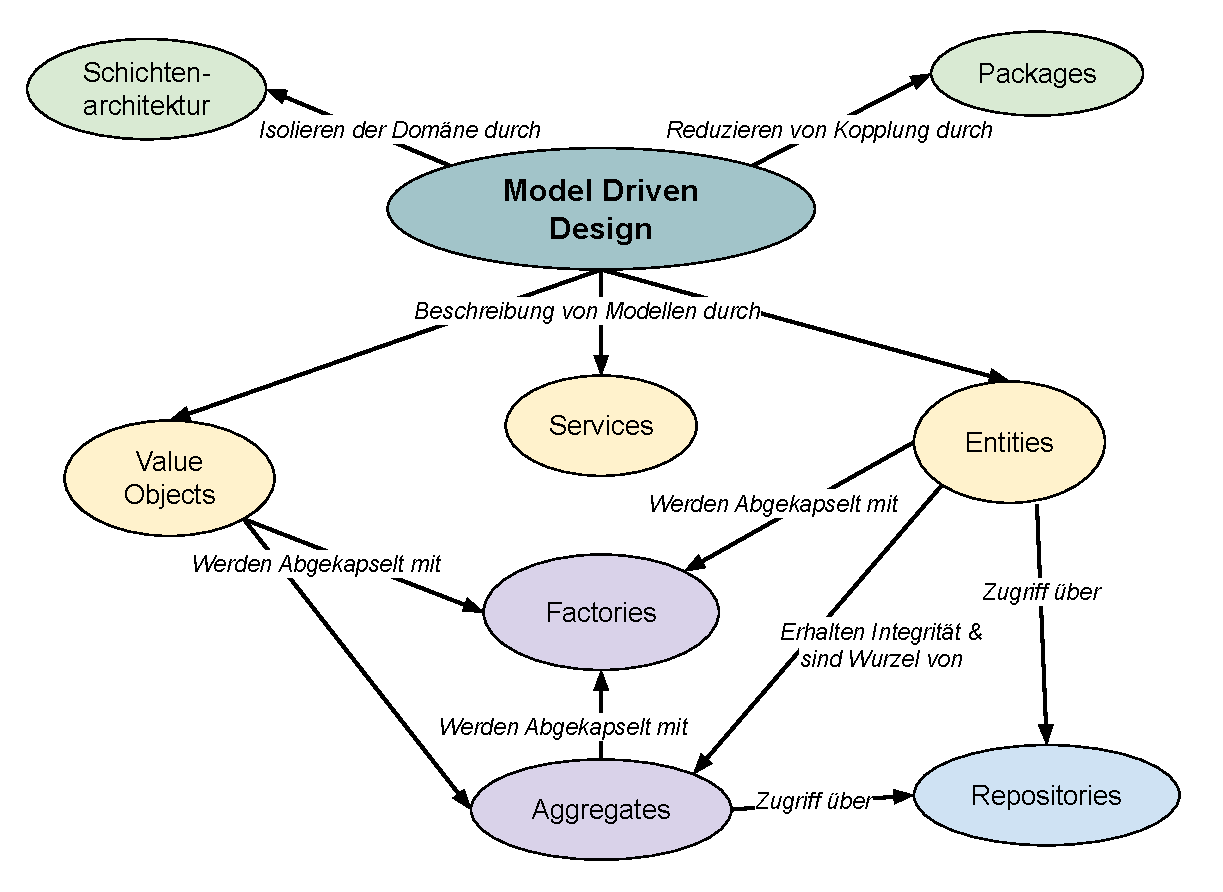
\includegraphics[width=\textwidth]{bilder/k2/MDD.pdf}
\caption[Bausteine des Model-Driven Design]{Die Bausteine des Model-Driven Design und wie Sie im Kontext zu anderen Bausteinen einzuordnen sind}
\end{figure}

\subsubsection{Schichtenarchitektur}


Der schichtbasierte Architekturstil teilt Software in verschiedene Schichten auf. Jede Schicht fasst Komponenten zusammen, die ähnliche Aufgaben haben. Das macht die Software einfacher zu verstehen und zu verwalten. Die Architektur ist nach technischen Funktionen gegliedert. Gängige Schichten sind die Präsentationsschicht, Geschäftslogikschicht, Persistenzschicht, Datenbankschicht oder die Dienstschicht. Jedes Element einer Schicht hängt nur von Elementen derselben oder einer tieferen Schicht ab. DDD fordert, die Geschäftslogik in eine eigene Schicht, der \glqq Domain Layer\grqq, zu legen. Dies sorgt für eine enge Verbindung zum Modell, wie es das MDD vorsieht \cite[S. 69 - 73]{evans} \cite[S.139-141]{richards}.


\subsubsection{Packages}

\glqq Packages\grqq, auch als \glqq Modules\grqq{} bezeichnet, sorgen im Modell für starke Kohäsion innerhalb und schwache Kopplung zwischen ihnen, indem sie zusammengehörige Elemente bündeln \cite[S. 109 - 116]{evans}.

\subsubsection{Entities}

\glqq Entities\grqq{} sind einzigartige, identifizierbare Objekte eines speziellen Bereichs. Dies kann z.B. mit automatisch erzeugten Identifikationswerten (Abk.: ID) umgesetzt werden. Ihre spezifischen Merkmale sind sekundär. Sie symbolisieren die durchgehende Existenz eines Objekts über dessen Lebenszyklus. Beim Erstellen eines Modells muss diese Kontinuität gewährleistet werden. Klassendetails, Aufgaben und Assoziationen sollten ebenso die Identität der Entity zeigen. Entities sollen sparsam verwendet werden. Nur notwendiges Verhalten soll ihnen hinzugefügt werden. Zusätzliches Verhalten soll zu anderen zugehörigen Objekten verschoben werden \cite[S. 89-96]{evans} \cite[S.75]{daschner}.

\subsubsection{Value Objects}

\glqq Value Objects\grqq{} sind Typen ohne eigene Identität, die spezifische Werte repräsentieren. Sie können aus anderen Value Objects bestehen und Entities referenzieren. Oft werden sie als Parameter zwischen Objekten oder als Eigenschaften von Entities genutzt. Value Objects sollten eine hohe Kohäsion besitzen und sind unveränderlich, um sicher geteilt werden zu können. Bidirektionale Verbindungen bei Value Objects sollten aufgrund ihrer fehlenden Identität vermieden werden \cite[S. 97-103]{evans} \cite[S.75]{daschner}.

\subsubsection{Services}

\glqq Services\grqq{} bieten eine spezielle Funktion im Modell an, ohne dabei Daten oder Zustände zu speichern. Sie werden dabei nach ihrer Aufgabe benannt. Services starten Vorgänge und arbeiten mit den Objekten des Modells. Sie kombinieren Schritte in Geschäftsprozessen und sollten bedacht eingesetzt werden. Außerdem sollen sie nicht alle Aufgaben von Entities und Value Objects abnehmen. Es existiert eine klare Schnittstelle im Bezug auf andere Elemente des Modells. Da Services auch außerhalb der Domain Layer auftreten können ist eine präzise fachliche Betrachtung nötig \cite[S. 104 - 108]{evans} \cite[S.74]{daschner}.

\subsubsection{Aggregates}

\glqq Aggregates\grqq{} sind Ansammlungen von Objekten, die zusammen als Einheit betrachtet werden. Ihr Zweck ist es, Veränderungen als Ganzes zu handhaben, um Konsistenz zu gewährleisten. Ein direkter Zugriff auf einzelne Bestandteile ist nicht möglich. Deswegen gibt es in einem Aggregate ein Hauptobjekt (Wurzel), das für alle Aktionen verwendet wird. Andere Objekte können nur auf dieses Hauptobjekt verweisen, wobei die enthaltenen Objekte sich untereinander gegenseitig verweisen können. Objekte innerhalb des Aggregates, die nicht die Hauptfunktion ausüben, sind nur in ihrem Kontext eindeutig identifizierbar \cite[S. 123 - 135]{evans} \cite[S.76]{daschner}.

\subsubsection{Factories}

Eine \glqq Factory\grqq{} erstellt Objekte. Dies ist nützlich, wenn das Erstellen eines Objekts mehr als nur das Ausführen eines Konstruktors beinhaltet, da manchmal besondere Regeln oder Logiken benötigt werden. Sie stellt sicher, dass jedes erstellte Objekt korrekt und vollständig ist. Auch wenn eine Factory dafür sorgt, dass ein Objekt richtig erstellt wird, kann sie Überprüfungen an andere Teile auslagern. Es gibt weiterhin Factories, die bestehende Objekte wiederherstellen. Dabei gibt es funktionale Unterschiede. Beispielsweiße weisen diese keine neuen IDs zu und müssen Verletzungen von Regeln anders behandeln \cite[S. 136 - 146]{evans} \cite[S.77]{daschner}.

\subsubsection{Repositories}

\glqq Repositories\grqq{} sind dafür zuständig, Daten von Entities oder Aggregates, sicher zu speichern und zu verwalten. Die Hauptidee von Repositories ist, einen zentralen Ort zu haben, der dafür sorgt, dass alles korrekt und konsequent gespeichert wird. Ein Repository ist mit einer Sammlung vergleichbar, aus der man Daten anhand von bestimmten Kriterien abfragen kann. Dabei fügt das Repository neue Objekte der Datenbank hinzu oder löscht sie. Wenn man Daten aus einem Repository möchte, nutzt man spezielle Suchmethoden. Dabei kann die Suche einfach oder auch sehr detailliert sein \cite[S. 147 - 161]{evans} \cite[S.76]{daschner}.

\subsubsection{Domain Event}

\glqq Domain Events\grqq{} sind Ereignisse, die für einen Geschäftsbereich relevant sind und zu einem Domänenmodell gehören. Sie entstehen aus Geschäftsvorfällen und haben eine spezifische Domänensemantik. In verteilten Systemen, wie zum Beispiel in Microservice-Architekturen, ergibt sich häufig die Notwendigkeit für Domain Events. Wenn in einem Microservice ein solches Ereignis eintritt, können andere Dienste an diesen interessiert sein. Eine Lösung hierfür ist, dass der betreffende Dienst ein Domain Event veröffentlicht, bei dem sich interessierte Dienste registrieren können. Dies fördert die Entkopplung der Dienste, da ihre Kommunikation hauptsächlich über Domain Events erfolgt \cite[S.78]{daschner} \cite{ritter}.

\pagebreak 
\subsection{Strategic Design}

Als \glqq Strategic Design\grqq{} wird im DDD beschrieben, wie verschiedene Domänenmodelle miteinander interagieren können. Dabei müssen die strategischen Designprinzipien die Designentscheidungen leiten, um Abhängigkeiten zu verringern und Klarheit zu erhöhen, ohne dabei Interoperabilität und Synergie zu gefährden \cite[S. 45]{wolff} \cite[S. 334]{evans}.

\subsubsection{Bounded Context}

Im Zentrum dieser Designentscheidungen steht der \glqq Bounded Context\grqq{}. Grundgedanke ist, dass jedes Domänenmodell nur in einem klar definierten Rahmen sinnvoll ist. Dieser Rahmen kann ein spezifischer Codebereich oder die Arbeit eines Teams sein. Der Bounded Context beschreibt Bedingungen, unter denen Begriffe im Modell eine bestimmte Bedeutung haben. Auch legen sie fest, in welchem Bereich ein Modell und somit auch die dazugehörige Ubiquitous Language gültig ist. Eine Domäne kann aus mehreren solchen Bounded Contexts bestehen. Bounded Contexts können auch Informationen mit anderen Bounded Contexts teilen. Jeder hat weiterhin eine Schnittstelle, die bestimmt, welche Modelle für andere Bounded Contexts verfügbar sind. Im Rahmen des Bounded Contexts sollte das Modell konsistent gehalten werden, um sich keine Sorgen um die Relevanz außerhalb dieser Grenzen machen zu müssen \cite[S. 45]{wolff} \cite[S.57]{newman} \cite[S. 335 - 340]{evans} \cite[S.64-65]{dowalil}.

\subsubsection{Shared Kernel}

Ein Bereich des Domänenmodells kann dazu dienen, zwischen Teams geteilt zu werden. Bei einem solchen \glqq Shared Kernel\grqq{} teilen sich die Domänenmodelle einige Elemente, können sich jedoch in anderen Aspekten unterscheiden. Dies kann entweder implizit oder explizit durch den gemeinsamen Codegebrauch bzw. durch den Zugriff auf dieselben Tabellen in der Datenbank geschehen. Oft bezeichnet der Shared Kernel die Kern-Domäne, eine Sammlung generischer Teilbereiche oder beides. Ziel dabei ist es, Wiederholungen zu vermeiden \cite[S. 354 - 355]{evans} \cite[S. 45]{wolff} \cite[S.65]{dowalil}.

\subsubsection{Customer/Supplier}

Zwischen zwei verschiedenen Kontexten kann eine Beziehung entstehen, die aus einer nachgelagerten und einer vorgelagerten Komponente besteht. Das Domain-Driven Design definiert deshalb eine klare Kunden-/Lieferantenbeziehung für solche Kontexte. Die \glqq Customer/Supplier\grqq{}-Beziehung zeigt, dass ein Untersystem dem Aufrufer ein Domänenmodell zur Verfügung stellt. Der Aufrufer, also der Kunde, legt die Struktur des Modells fest. Der Anbieter der Schnittstelle richtet sich beim Design nach den Wünschen des Kunden und gibt ihm oft ein Mitspracherecht \cite[S. 356 - 360]{evans} \cite[S. 45,47]{wolff} \cite[S.66]{dowalil}.

\subsubsection{Conformist}

Wenn die Anforderungen eines nachgelagerten, abhängigen Subsystems durch den vorgelagerten Teil gedeckt werden können, bietet es sich an, dem nachgelagerten Teil die Rolle des \glqq Conformist\grqq{} zuzuweisen. Dies vereinfacht den Datenaustausch zwischen den beiden Kontexten, indem beide dasselbe Modell verwenden. Der Aufrufer nutzt also das gleiche Modell wie das aufgerufene System und passt sich somit dem anderen Modell an \cite[S. 361 - 363]{evans} \cite[S. 47]{wolff} \cite[S.66]{dowalil}.

\subsubsection{Anticorruption Layer}

Wenn man Systeme kombiniert, die auf verschiedenen Modellen basieren, kann es passieren, dass das Modell des einen Systems durch das andere beeinflusst wird. Ein \glqq Anticorruption Layer\grqq{} hilft, indem es eine Schutzschicht bildet. Diese Schicht ermöglicht es den Nutzern, mit ihrem gewohnten Modell zu arbeiten, ohne das andere System zu beeinflussen. Sie dient als Übersetzer zwischen den beiden Modellen und sorgt dafür, dass sie unabhängig voneinander bleiben. Über eine Schnittstelle kommuniziert sie mit dem anderen System, ohne dass große Änderungen an diesem notwendig sind. Sie kann bei Bedarf in beide Richtungen übersetzen \cite[S. 364 - 370]{evans} \cite[S. 47]{wolff} \cite[S.66]{dowalil}.

\subsubsection{Separate Ways}

Wenn der Nutzen im Vergleich zu den Integrationskosten zu gering ist, kann es sinnvoll sein, festzulegen, dass ein bestimmter Kontext keine Verbindung zu anderen hat. Im DDD spricht man hier von \glqq Separate Ways\grqq{}, was bedeutet, dass die beiden Systeme nicht verbunden werden und unabhängig voneinander bleiben. Anstatt Lösungen für Probleme gemeinsam zu nutzen, müssen diese auf einem klaren, speziellen Weg innerhalb dieses Rahmens umgesetzt werden. \cite[S. 371 - 373]{evans} \cite[S. 47]{wolff} \cite[S.66]{dowalil}.


\subsubsection{Open Host Service}

Wenn ein Teilsystem mit vielen anderen verbunden werden muss, kann es problematisch sein, für jedes einen Übersetzer anzupassen. Hier bietet es sich an, ein offenes Protokoll von Diensten zu definieren, das Zugang zum Teilsystem ermöglicht. Dieser Kontext, als \glqq Open Host Service\grqq{} bezeichnet, stellt also Schnittstellen bereit, die jeder nutzen kann. So kann jeder Kontext seine eigene Anbindung erstellen.
\cite[S. 374]{evans} \cite[S. 48]{wolff} \cite[S.66]{dowalil}.

\subsubsection{Published Language}

Das direkte Übersetzen von Modellsprachen kann zu sehr komplexen Strukturen führen. Selbst wenn eine Sprache für den Datenaustausch genutzt wird, ist sie einmal festgelegt und lässt sich nicht leicht an Entwicklungsbedürfnisse anpassen. Deshalb kann eine gut dokumentierte, gemeinsame Sprache als allgemeines Kommunikationsmittel bereitgestellt werden. Diese \glqq Published Language\grqq stellt eine Modellierung der Domäne als universelle Sprache zwischen den Bounded Contexts dar \cite[S. 375-378]{evans} \cite[S. 48]{wolff} \cite[S.65]{dowalil}.

\subsubsection{Context Map}

Eine \glqq Context Map\grqq{} liegt an der Schnittstelle zwischen Projektmanagement und Softwareentwurf. Sie ist eine grafische Übersicht über bestehende Modelle, wobei der Fokus auf den Berührungspunkten liegt. Diese macht explizit die Kommunikationswege und gemeinsam genutzten Bereiche deutlich. Context Maps werden verwendet, um die Beziehungen verschiedener Bounded Contexts darzustellen \cite[S. 344 - 353]{evans} \cite[S. 45]{wolff}.

\begin{figure}[ht]
\centering
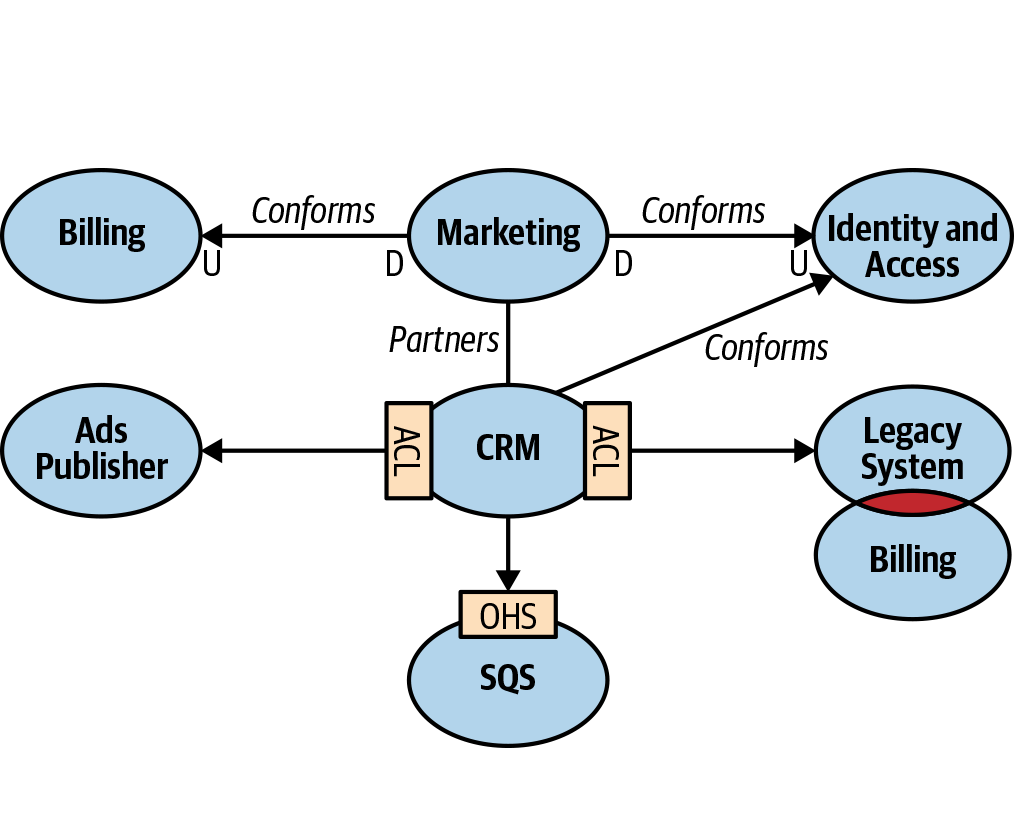
\includegraphics[width=0.8\textwidth]{bilder/k2/k2_context_map.png}
\caption[Darstellung von Bounded Contexts und ihre Rollen in der Context Map]{Darstellung von Bounded Contexts und ihre Rollen zueinander in einer Context Map \cite{oreillymap}}
\end{figure}


%%%%%%%%%%%%%%%%%%%%%%%%%%%%%%%%%%%%%%%%%%%%%%%%%%%%%%%%%%%%%%%%%%%%%%%%%%%%%%%%%%%%%%%%%%%%%%%%%%%%%%%%%%%%%%%
%
%						MICROSERVICES
%
%%%%%%%%%%%%%%%%%%%%%%%%%%%%%%%%%%%%%%%%%%%%%%%%%%%%%%%%%%%%%%%%%%%%%%%%%%%%%%%%%%%%%%%%%%%%%%%%%%%%%%%%%%%%%%%

\pagebreak
\section{Microservices}

\subsection{Geschichte und Definition}

Im Mai 2011 wurde der Begriff \glqq Microservice\grqq{} während eines Architekten-Workshops in Venedig eingeführt, um einen neu entstehenden Architekturstil zu beschreiben. Dieser Stil entwickelte sich aus der \glqq Service-orientierten Architektur\grqq{} (Abk.: SOA). Ein Software-Service bezeichnet in der SOA eine Softwarekomponente, die über das Internet von entfernten Computern aus zugänglich ist. Microservice-Architekturen ähneln der SOA, aber SOA wird oft unterschiedlich verstanden und unterscheidet sich in der Regel von Microservices. Merkmale von SOA-Architekturen sind unter anderem ein zentraler Zugriffsbus (ESB) oder die Abbildung ganzer Geschäftsabläufe in einem Service.

Viele SOA-Projekte stoßen wegen ihrer Komplexität oder hohen Kosten auf Schwierigkeiten. Aufgrund von Herausforderungen bei Skalierung und Verschiebung der Services entstand ein neuer Ansatz: Ein völlig unabhängiger Dienst mit eigener Datenbank, eigener Benutzeroberfläche und der Fähigkeit, einen Dienst zu ersetzen oder zu replizieren, ohne andere Systemdienste ändern zu müssen. Ein Jahr später wurde der Name Microservices als am besten passend für dieses Konzept gewählt. Der Microservice-Architekturstil wurde dann von Martin Fowler und James Lewis im März 2014 in einem Blogbeitrag erstmals ausführlicher vorgestellt \cite{fowlerlewis} \cite[S.251]{richards}. \cite[S.150,151]{sommerville}.

Microservices wurden nicht im Voraus geplant, sondern entstanden durch beobachtete Trends und Muster in der Praxis. Dazu gehören Continuous Delivery, bedarfsorientierte Virtualisierung, automatisierte Infrastrukturen, skalierbare Systeme und unabhängige Entwicklerteams. Die Hauptinspiration stammt jedoch aus dem DDD, insbesondere dem Konzept des Bounded Context \cite[S.21]{newman} \cite[S.251]{richards}.

Microservices können als kleine, leicht ersetzbare, unabhängige Komponenten definiert werden, die sich auf eng begrenzte Geschäftsvorgänge konzentrieren. Ihr Hauptziel ist eine hohe Entkopplung \cite[S.252]{richards} \cite[S.5,6]{fowlersusan} \cite[S.152]{sommerville} \cite[S.113]{erl} \cite[S.22-23]{newman}.

\pagebreak
\subsection{Eigenschaften von Microservices}

Verschiedene Eigenschaften zeichnen einen Microservice aus:

\begin{figure}[ht]
\centering
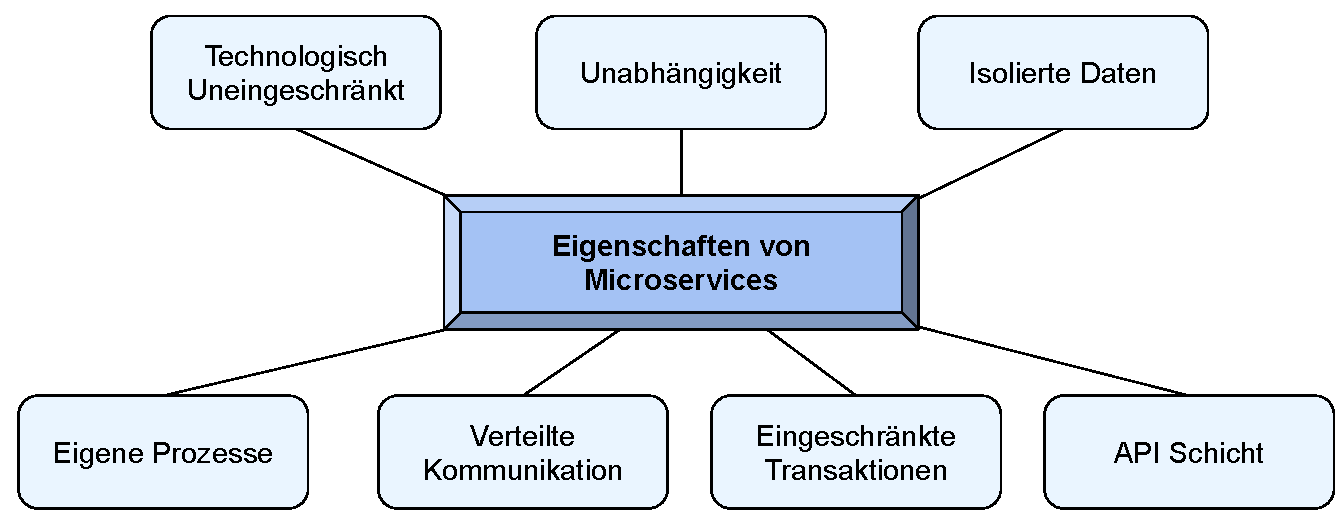
\includegraphics[width=\textwidth]{bilder/k2/eigenschaften.pdf}
\caption[Eigenschaften von Microservices]{Die verschiedenen Eigenschaften von Microservices}
\end{figure}

\subsubsection{Technologisch Uneingeschränkt}

In ihrer Implementierung können Microservices unabhängig voneinander mit verschiedenen Technologien umgesetzt werden. Es existieren keine technologischen Einschränkungen \cite[S. 2, 31-37]{wolff} \cite[S.154-157]{sommerville} \cite[S.24]{newman}.

\subsubsection{Unabhängigkeit}

Der Ansatz von Microservices zielt darauf ab, Services für eng begrenzte Geschäftsvorgänge zu erstellen, die unabhängig voneinander geändert und bereitgestellt werden können.Der Fokus liegt auf Ersetzbarkeit statt Wiederverwendung. Automatisierte Builds und Deployments vereinfachen dies. \cite[S. 2, 31-37]{wolff} \cite[S.22,23,28]{newman} \cite[S.154-157]{sommerville} \cite[S.128]{dowalil}.
 
\subsubsection{Isolierte Daten}

Microservices, die auf dem Konzept des Bounded Contexts basieren, legen Wert auf Datenisolierung. Sie vermeiden jegliche Formen der Kopplung, einschließlich gemeinsam genutzter Schemata und Datenbanken als Integrationspunkte, und verfügen über einen eigenen Datenhaushalt auf ihrer ausführenden Infrastruktureinheit \cite[S. 2, 31-37]{wolff} \cite[S.255]{richards}.

\subsubsection{Eigene Prozesse}

Ein Microservice ist wie ein eigenständiges Programm, das entweder als eigener Dienst auf einer Plattform oder als eigener Prozess auf einem Betriebssystem läuft. Jeder dieser Dienste arbeitet unabhängig und kann automatisch und einzeln bereitgestellt werden \cite[S.23]{newman} \cite[S.253]{richards} \cite[S. 2, 31-37]{wolff} \cite[S.154-157]{sommerville}.

\subsubsection{Verteilte Netzwerkkommunikation}
Microservices repräsentieren eine verteilte Architektur und nutzen verteilte Netzwerkkommunikation für die Interaktion mit anderen Diensten. Die Integration der Services erfolgt hauptsächlich über REST oder Lightweight Messaging. Durch die Kommunikation über leichte Protokolle wird der Zusatzaufwand minimiert. Die Netzwerkkommunikation betont die Isolierung der Services und vermeidet die Gefahren einer engen Kopplung \cite[S.253]{richards} \cite[S. 2, 31-37]{wolff} \cite[S.154-157]{sommerville} \cite[S.128]{dowalil} \cite[S.23]{newman}.

\subsubsection{Einschränkungen bei Transaktionen}

Aufgrund dieser Architektur, sollten Transaktionen nicht über mehrere Services hinweg durchgeführt werden. Transaktionen sind durch die ACID-Eigenschaften (Atomizität, Konsistenz, Isolation, Dauerhaftigkeit) gekennzeichnet \cite[S.253]{richards} \cite[S. 2, 31-37]{wolff}.

\subsubsection{API-Schicht}

In vielen Darstellungen von Microservices ist eine API(Application Programming Interface)-Schicht erkennbar, die zwischen den Nutzern und dem System liegt. Obwohl diese Schicht optional ist, wird sie häufig verwendet, da sie in der Architektur gut positioniert ist, um nützliche Aufgaben zu erfüllen. Sie sollte jedoch nicht als Vermittler oder Orchestrierungswerkzeug fungieren, da Microservices streng domänenspezifisch sind. Jeder Service stellt eine API bereit, über die andere Services mit ihm kommunizieren können. Es ist wichtig, dass durch die API keine Kopplung an die Nutzer entsteht, was bei der Technologieauswahl zu berücksichtigen ist \cite[S.255,256]{richards} \cite[S.24]{newman}.

\pagebreak
\subsection{Architektur von Microservice-Systemen}

Microservices sind kleine Dienste, die zusammengesetzt Anwendungen bilden. Sie unterscheiden sich von traditionellen, geschichteten Architekturen. Statt einer festgelegten Menge von Komponenten, setzen sie auf flexiblere, unabhängige Dienste. In der Softwareentwicklung gibt es den Trend, Systeme modular zu gestalten. Microservice-Architekturen tun dies, indem sie Software in Dienste statt in klassische Bibliotheken gliedern. Vorteile sind unter anderem die unabhängige Bereitstellung und klare Schnittstellen, die eine enge Verknüpfung vermindern \cite[S.154-157]{sommerville} \cite{fowlerlewis}.

\subsubsection{DDD-Prinzipien}

Der Kerngedanke hinter Microservices ist der Bounded Context. Jeder Dienst repräsentiert eine Domäne oder einen bestimmten Arbeitsprozess. Ein Microservice sollte eine eigenständige fachliche Einheit darstellen, die so gestaltet ist, dass bei Änderungen oder neuen Funktionen nur dieser eine Microservice angepasst werden muss. Ein Bounded Context kann in mehrere Microservices unterteilt werden, falls das zweckmäßig ist. Zudem sollten die aus dem DDD bekannten Konzepte des Strategic Design berücksichtigt werden. Die Zuständigkeiten der Anwendungen müssen daher klar definiert und von anderen Anwendungen abgegrenzt sein \cite[S.253,254]{richards} \cite[S. 48-51]{wolff} \cite[S.289]{daschner}.

\subsubsection{Kopplung und Kohäsion}

Kohäsion beschreibt, wie eng Teile eines Moduls zusammengehören sollten \cite[S.40]{richards}. Kopplung hingegen zeigt, wie stark eine Komponente von einer anderen abhängt \cite[S.44]{richards}. Das Ziel bei Microservices ist es, einen Dienst mit starker Kohäsion und schwacher Kopplung zu schaffen. Dies basiert auf dem \glqq Single Responsibility Principle\grqq{} \cite[S.154-157]{sommerville}.

Innerhalb eines Dienstes sollten die Bestandteile eng zusammenarbeiten (hohe Kohäsion). Zwischen den Microservices sollte eine schwache Kopplung herrschen, sodass sie unabhängig und leicht änderbar sind. Wenn Dienste schwach gekoppelt sind, bedeutet das, dass eine Änderung in einem Dienst nicht automatisch Änderungen in anderen erfordert. Ein schwach gekoppelter Dienst kennt nur das Nötigste über andere Dienste. Deshalb ist es ratsam, die Kommunikation zwischen den Diensten zu beschränken, um Geschwindigkeitsprobleme und enge Kopplungen zu vermeiden. Zyklische Abhängigkeiten in der Architektur sind problematisch, da sie die Unabhängigkeit der Änderungen beeinträchtigen \cite[S. 101-105]{wolff} \cite[S.56]{newman}.

Das Ausrichten von Microservice-Schnittstellen auf spezifische Kontexte schafft optimale Voraussetzungen für schwache Kopplung und starke Kohäsion \cite[S.59,60]{newman}.

\subsubsection{Ereignisgetriebene Architektur in Microservices}

Um gemeinsame Logik zu implementieren, müssen Microservices miteinander kommunizieren. Dadurch werden größere Transaktionen in kleinere aufgeteilt, die zwar für sich genommen inkonsistent sein können, aber im Gesamtkontext für Konsistenz sorgen. Eine ereignisgetriebene Architektur (Event-Driven Architecture, Abk.: EDA) kann hierbei helfen. Bei dieser Architektur sendet ein Dienst, bei einem bestimmten Ereignis, eine Nachricht aus. Dieser Dienst, der \glqq Event-Emitter\grqq, informiert so alle beteiligten Microservices darüber, dass eine Aktion stattgefunden hat. Der eventbasierte Architekturstil arbeitet verteilt und asynchron. In dieser Architektur erfolgt die Kommunikation über asynchrone Nachrichten, die zuverlässig gesendet und empfangen werden. Die Komponenten sind entkoppelt und verarbeiten diese Nachrichten asynchron \cite[S. 137 - 138]{wolff} \cite[S.183]{richards} \cite[S.301]{daschner}.

Für die Ereignisgetriebene Architektur existieren zwei grundlegende Topologien: Die \glqq Broker-Topologie\grqq{} und die \glqq Mediator-Topologie\grqq.

\begin{figure}[ht]
\centering
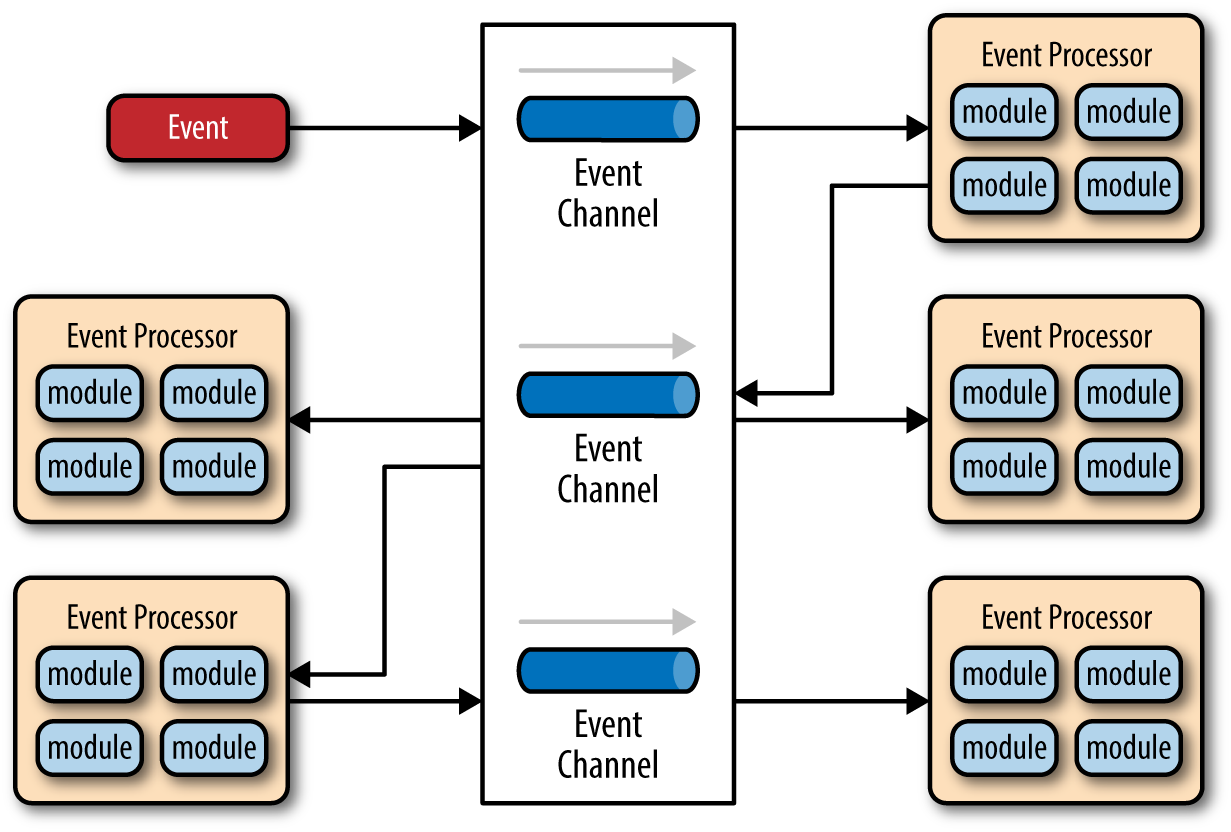
\includegraphics[width=0.7\textwidth]{bilder/k2/k2_broker.png}
\caption[Darstellung einer Broker-Topologie in der EDA]{Eine Broker Topologie mit einem Message Broker und verschiedenen Event-Prozessoren \cite{richards}}
\end{figure}

In der Broker-Topologie verteilt ein \glqq Message Broker\grqq{} Nachrichten über die Event-Prozessoren, ähnlich einem verketteten Broadcasting. Diese Topologie ist sinnvoll, wenn eine hohe Reaktionsfähigkeit und dynamische Kontrolle über die Eventverarbeitung gefordert sind. Sie ist besonders nützlich, wenn der Event-Verarbeitungsfluss einfach ist und keine zentrale Orchestrierung oder Koordination benötigt.

Die Broker-Topologie besteht aus vier Hauptkomponenten: Einem auslösenden Event, dem Event-Broker, einem Event-Prozessor und einem verarbeitenden Event.

Das auslösende Event startet den Event-Fluss und wird zur Verarbeitung an einen Kanal des Event-Brokers weitergeleitet. Ein einzelner Event-Prozessor übernimmt und verarbeitet das Event. Nach der Verarbeitung informiert er das System über ein sogenanntes Verarbeitungs-Event über seine Aktionen. Dieses wird asynchron an den Event Broker gesendet, um eventuell weitere Verarbeitungsschritte zu initiieren. Andere Event-Prozessoren reagieren darauf, führen Aktionen aus und informieren das System erneut über ein Verarbeitungs-Event. Dieser Prozess wiederholt sich, bis kein weiteres Interesse an den Aktionen des letzten Event-Prozessors besteht.

Ein Event-Broker ist oft in Domänen unterteilt, wobei jeder Broker alle für eine Domäne notwendigen Kanäle enthält. In der Broker-Topologie wird ein entkoppeltes, asynchrones \glqq fire and forget\grqq{} Broadcasting mit \glqq Topics\grqq{} verwendet, die nach dem \glqq Publish-Subscribe\grqq{}-Modell funktionieren. Jeder Event-Prozessor teilt dabei dem System mit, was er getan hat, unabhängig davon, ob dies für andere Event-Prozessoren relevant ist oder nicht \cite[S.184-186]{richards}.

\begin{figure}[ht]
\centering
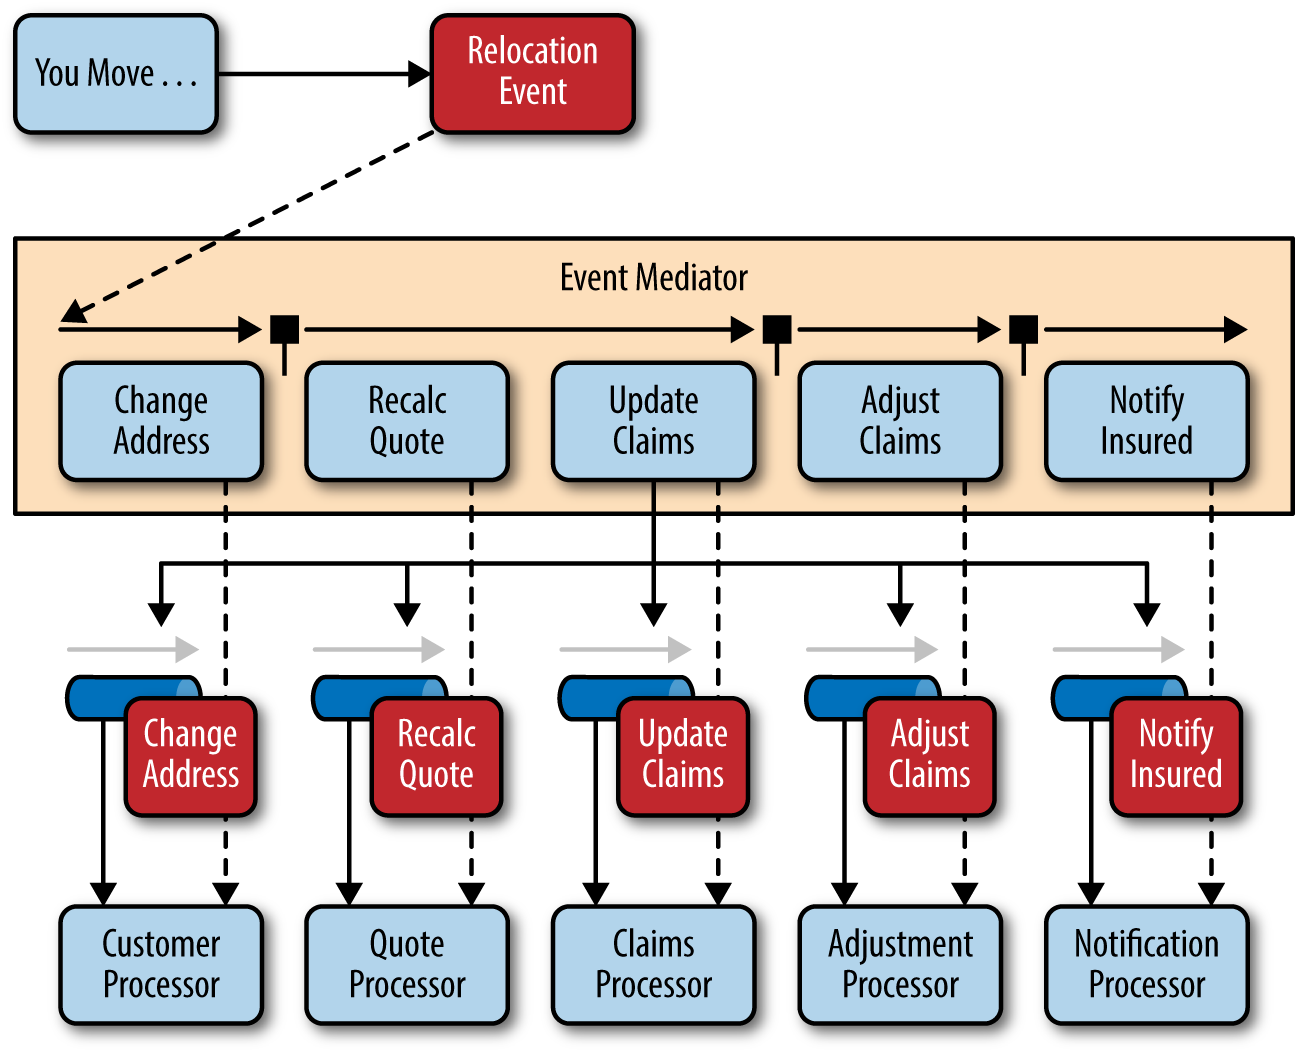
\includegraphics[width=0.7\textwidth]{bilder/k2/k2_mediator.png}
\caption[Darstellung einer Mediator-Topologie in der EDA]{Eine Mediator Topologie mit einem Message Broker und verschiedenen Event-Prozessoren \cite{richards}}
\end{figure}

Die Mediator-Topologie verfügt über einen \glqq Event-Mediator\grqq, der den Arbeitsablauf und die beteiligten Event-Prozessoren für initiale Events steuert. Sie setzt sich zusammen aus einem initialen Event, einer \glqq Event-Queue\grqq, dem Event-Mediator, Event-Kanälen und Event-Prozessoren.

In dieser Topologie wird das initiale Event zuerst an die Event-Queue gesendet, die vom Event-Mediator verwaltet wird. Der Event-Mediator kennt nur die für die Event-Verarbeitung erforderlichen Schritte und erzeugt daher Verarbeitungs-Events, die zu den jeweiligen Event-Kanälen weitergeleitet werden. Die Event-Prozessoren hören auf bestimmten Event-Kanäle, bearbeiten das Event und informieren in der Regel den Event-Mediator nach Abschluss ihrer Aufgabe. Anders als bei einer Broker-Topologie teilen die Event-Prozessoren nicht mit, was sie verarbeitet haben. Häufig gibt es verschiedene Mediatoren, die jeweils für bestimmte Bereiche oder Event-Gruppen verantwortlich sind \cite[S.189-190]{richards}.

\pagebreak
\subsection{Kommunikation}

In einer Microservice-Architektur ist es möglich, die Kommunikation entweder synchron oder asynchron zu gestalten. Bei synchroner Kommunikation wartet der aufrufende Dienst auf eine Rückmeldung des aufgerufenen Dienstes. Diese Wartezeit blockiert den Aufrufer, bis die Transaktion abgeschlossen ist. Synchroner Datenaustausch gilt generell als weniger komplex im Vergleich zur asynchronen. Bei asynchroner Kommunikation hingegen muss der aufrufende Dienst nicht auf die Fertigstellung der Transaktion warten. Für den Aufrufer kann es unter Umständen unerheblich sein, ob die Anfrage vollständig bearbeitet wird oder nicht. Asynchrone Kommunikation ist oftmals effizienter, da die beteiligten Services nicht untätig während dem Warten sind. Zudem erleichtert die lose Kopplung bei ausschließlich asynchron kommunizierenden Services deren Modifikation \cite[S.260,261]{richards} \cite[S.161-163]{sommerville} \cite[S.70-71]{newman}.

\subsubsection{REST}

Der REST(Representational State Transfer)-Architekturstil ermöglicht die Übertragung von Ressourcen von einem Server zu einem Client. In diesem Zusammenhang bezeichnet eine Ressource ein Objekt, das dem Service bekannt ist. Die Art und Weise, wie eine Ressource nach außen präsentiert wird, ist unabhängig von ihrer internen Darstellung. Beziehungen zwischen Ressourcen können durch Links repräsentiert werden, was dem Prinzip von \glqq HATEOAS\grqq(Hypermedia as the Engine of Application State) entspricht. REST selbst macht keine spezifischen Angaben zum verwendeten Protokoll. Allerdings wird am häufigsten HTTP eingesetzt. Ein \glqq RESTful-Service\grqq{} nutzt die im HTTP-Protokoll definierten Methoden \cite{http} und arbeitet zustandslos. Zu den Operationen eines RESTful-Services gehören das Erstellen (umgesetzt mit \glqq POST\grqq), das Lesen (umgesetzt mit \glqq GET\grqq), das Aktualisieren (umgesetzt mit \glqq PUT\grqq) und das Löschen (umgesetzt mit \glqq DELETE\grqq) von Ressourcen. RESTful HTTP arbeitet synchron. Durch die Verwendung von Zeitüberschreitungen können Probleme wie Serverausfälle adressiert werden \cite[S.79-80]{newman} \cite[S. 182 - 183]{wolff} \cite[S.173-175]{sommerville}.

\subsubsection{Messaging}

Messaging-Systeme ermöglichen eine asynchrone Kommunikation zwischen Microservices. Ihr Hauptmerkmal ist das Versenden von Nachrichten, die sogar bei einem Netzwerkausfall übermittelt werden können. Dies wird durch das Zwischenspeichern der Nachrichten in den Messaging-Systemen erreicht. Bei Auftreten eines Fehlers sorgt die Möglichkeit, eine Übertragung erneut zu initiieren, für eine korrekte Verarbeitung. Ein wichtiger Vorteil ist, dass der Aufruf eines anderen Services die weitere Verarbeitung nicht blockiert, wodurch ein Microservice ohne Verzögerung auf eine Antwort weiterarbeiten kann. Im Messaging-System ist der Sender der Nachrichten typischerweise anonym, da diese auf einer Queue oder einem Topic landen, auf die sich interessierte Empfänger registrieren können. Apache Kafka ist eine Technologie mit der Messaging implementiert werden kann \cite[S. 183 - 187]{wolff} \cite[S.87-88]{newman}.

\pagebreak 
\subsection{Betrieb}

In der Vergangenheit waren Betrieb und Entwicklung eines Systems klar voneinander getrennte Bereiche, die jeweils spezifische Aufgaben für Systemadministratoren und Entwickler mit sich brachten. Heute jedoch erfordern komplexe, aus vielen Microservices bestehende und über die Cloud verteilte Systeme eine konsistente und einheitliche Verwaltung. Diese verteilten Systeme basieren auf dem Einsatz von virtuellen Maschinen und Containern. Tools wie Kubernetes leisten wertvolle Dienste bei der Planung, der Verteilung von Arbeitslasten und im Management von Docker-Containern. Nachdem ein System entwickelt und in Betrieb genommen wurde, sind kontinuierliches Monitoring und regelmäßige Updates unerlässlich. Im Bereich der Softwaretechnik bezeichnet Monitoring das Überwachen von Metriken, um Zustand und Leistung einer Software zu analysieren und zu verstehen. Zu den wichtigsten Metriken zählen dabei Host- und Infrastrukturdaten wie CPU- und RAM-Auslastung, Thread-Anzahl, offene Dateideskriptoren und Datenbankverbindungen jedes einzelnen Microservices. Aufgrund der dynamischen Natur von Microservices, deren Instanzen jederzeit gestartet oder beendet werden können, ist es entscheidend, dass das Monitoring sowohl systemübergreifend als auch unabhängig vom jeweiligen Dienst funktioniert. Technologien wie Graphite, Grafana oder Nagios sind hierfür geeignete Werkzeuge. Auch Cloud-Umgebungen bieten spezielle Tools, um ein leistungsfähiges und effizientes Monitoring zu gewährleisten \cite[S.158,179,181]{sommerville} \cite[S.253]{richards} \cite[S. 80-81, S.250-256, S.263-269]{wolff} \cite[S.105-108]{fowlersusan}.

\subsection{Microservices mit Spring Boot}

Microservices lassen sich effektiv mit dem Java-Framework Spring Boot realisieren, welches auf dem Spring Framework basiert. Zur Verwaltung von Abhängigkeiten in einem Spring Boot-Projekt werden Build-Management-Tools wie Maven oder Gradle verwendet. So werden bei Gradle in der build.gradle-Datei sämtliche Abhängigkeiten sowie spezifische Besonderheiten für die Kompilierung definiert. Innerhalb von Gradle werden verschiedene Abschnitte des Build-Prozesses, wie das Kompilieren oder Testen, als Tasks bezeichnet.

Ein Schlüsselkonzept des Spring Frameworks ist die Dependency Injection. Hierbei instanziieren oder referenzieren Objekte ihre erforderlichen Kollaborateure nicht selbst. Stattdessen stellt das Framework diese von außen bereit. Um auf diese Weise instanziert werden zu können, müssen Klassen als Komponenten gekennzeichnet sein. Das Spring Framework bietet zudem diverse Module für zusätzliche Funktionalitäten. So ermöglicht das Spring MVC-Modul durch Annotationen die Zuordnung von URLs zu Methoden, was besonders bei der Implementierung von REST-Schnittstellen nützlich ist. Spring Data JPA erleichtert das Mapping von Java-Klassen auf Datenbankobjekte. Das Spring Webflux-Modul stellt mit dem \glqq WebClient\grqq eine Implementierung für das Stellen von HTTP-Anfragen bereit \cite[S.30-39,S.54-58, S.130-139, S.220-227, S.279-281]{simons}. Die breite aller Funktionalitäten von Spring und Spring Boot lässt sich detailliert in der offiziellen Dokumentation einsehen \cite{spring} \cite{springboot}.



%%%%%%%%%%%%%%%%%%%%%%%%%%%%%%%%%%%%%%%%%%%%%%%%%%%%%%%%%%%%%%%%%%%%%%%%%%%%%%%%%%%%%%%%%%%%%%%%%%%%%%%%%%%%%%%
%
%						CLOUD-INFRASTRUKTUR
%
%%%%%%%%%%%%%%%%%%%%%%%%%%%%%%%%%%%%%%%%%%%%%%%%%%%%%%%%%%%%%%%%%%%%%%%%%%%%%%%%%%%%%%%%%%%%%%%%%%%%%%%%%%%%%%%

\pagebreak 
\section{Cloud-Computing}

Cloud-Computing bedeutet, Rechnerressourcen über ein Netzwerk zu nutzen. Mithilfe von Virtualisierung lassen sich die Ressourcen eines von Cloud-Anbietern betriebenen Rechenzentrums abgrenzen. Das National Institute of Standards and Technology (NIST) beschreibt Cloud-Computing als ein Modell für einen allgegenwärtigen, bequemen und bedarfsgerechten Netzwerkzugang zu einem Pool von konfigurierbaren Rechenressourcen, die schnell und mit minimalem Verwaltungsaufwand oder ohne große Interaktion mit dem Dienstanbieter bereitgestellt und freigegeben werden können \cite[S. 20]{stender} \cite[S.19-22]{riti} \cite{nist}.

\subsection{Docker}

Softwarecontainer sind eine Methode, Anwendungen in standardisierte und portable Einheiten zu verpacken, die autonom funktionieren. Das Besondere an diesen Umgebungen ist ihre Isolation vom restlichen System, wobei sie als abgegrenzte Prozesskapseln innerhalb definierter Grenzen operieren. Diese Isolation ermöglicht den Betrieb unterschiedlicher Anwendungen und sogar verschiedener Komponenten einer Anwendung in separaten Containern, die in der Cloud individuell skaliert werden können. Dieses Prinzip findet im Bereich der Microservices sowohl in der Entwicklung als auch in der Applikationsarchitektur intensive Anwendung.

Die Containerisierung kann als eine Evolution der Virtualisierung betrachtet werden, bei der ein Betriebssystem auf einem Hostrechner simuliert wird. Es existieren hauptsächlich zwei Arten von Containern: System-Container, die virtuelle Maschinen nachahmen und oft einen vollständigen Boot-Prozess durchlaufen, sowie Anwendungscontainer, die in der Regel nur ein einzelnes Programm ausführen. Docker, als die wohl bekannteste Container-Software, bietet eine Virtualisierung auf Betriebssystemebene, die mit Containerisierung vergleichbar ist. Diese Technik der Isolation ermöglicht es, mehrere Betriebssysteme innerhalb eines anderen Betriebssystems zu betreiben \cite[S. 54-59]{stender} \cite[S.18]{burns1} \cite[S.63]{riti}.

\glqq Images\grqq{} bilden das Kernstück der Docker-Architektur und sind essentiell für das Starten von Containern. Man kann eigene Images erzeugen, indem man von einem Basismodell ausgeht. Jedes Container-Image stellt ein Binärpaket dar, welches sämtliche für die Ausführung eines Programms in einem Betriebssystemcontainer erforderlichen Dateien beinhaltet. Das Docker-Image-Format hat sich mittlerweile als Industriestandard durchgesetzt. Die Erstellung eines Docker-Container-Images lässt sich durch ein Dockerfile automatisieren. In der Praxis ist ein Container ein in Betrieb genommenes Image, das je nach Konfiguration und Aufbau des Images mehrere Prozesse beherbergen kann. Durch die Kombination mehrerer Container können komplexe Anwendungen realisiert werden. Als \glqq Registry\grqq{} bezeichnet man den Speicherort für Images, wobei zwischen privaten und öffentlichen Registries unterschieden wird \cite[S.16-18]{burns1} \cite[S.64-65]{riti}.

\subsection{Kubernetes}

Für die Orchestrierung einer komplexen, containerbasierten Anwendung in einem \glqq Cluster\grqq{} ist ein Cluster-Manager notwendig. Ein Cluster besteht aus einer Gruppe von Servern, die Container enthalten und als Knoten bezeichnet werden. Beispiele für Cluster-Manager sind Docker Swarm oder Kubernetes, wobei letzteres nachfolgend detaillierter betrachtet wird:

Kubernetes, ein von Google entwickeltes und von der Cloud Native Computing Foundation verwaltetes Open-Source-System, dient dem Deployment containerbasierter Anwendungen. Es ermöglicht die Verwaltung und Skalierung solcher Anwendungen innerhalb eines Clusters und hat sich als moderner Standard für den verteilten Betrieb von Applikationen etabliert, insbesondere in bereitgestellten Cloud-Umgebungen. Dabei verwendet Kubernetes standardmäßig Docker als Container-Engine. Über eine eigene API, die vor allem in der Entwicklung spezifischer Werkzeuge Anwendung findet, bietet Kubernetes umfassende Steuerungsmöglichkeiten. Ein Kubernetes-Cluster setzt sich aus Knoten (Nodes) zusammen, die in einen Master-Knoten und beliebig viele Worker-Knoten untergliedert sind. Ein Cluster kann dabei ausschließlich aus einem Master-Knoten bestehen, wobei jeder Knoten je nach Konfiguration als Master oder Worker fungieren kann. Kubernetes basiert auf dem Prinzip deklarativer Konfigurationsobjekte, die den angestrebten Zustand des Systems beschreiben. Der Ansatz, deklarative Konfigurationen unter Versionskontrolle zu halten, ist auch als \glqq Infrastructure as Code\grqq bekannt. Mit dem Werkzeug kubectl interagieren Benutzer über die auf dem Master-Knoten laufende API mit dem Cluster. Der Master-Knoten steuert die Worker-Knoten und setzt die vom Benutzer gewünschten Änderungen um \cite[S.1,4]{burns1} \cite{burns3} \cite[S.79,81]{riti} \cite[S. 60-63,166]{stender}.

Kubernetes definiert eine Reihe grundlegender Objekte, die zur Erstellung und Verwaltung von Ressourcen dienen. Diese Komponenten sind flexibel konzipiert, sodass sie miteinander kombiniert werden können. Innerhalb von Kubernetes repräsentieren Objekte verschiedene Elemente, die im Cluster genutzt werden. Jedes dieser Objekte verfügt über einen einzigartigen HTTP-Pfad, da sie in Kubernetes alle als REST-Ressourcen abgebildet werden \cite[S.40, 42]{burns1} \cite[S.80-81]{riti} \cite[S. 166-192]{stender}.

\subsubsection{Deployment}

Ein Deployment ist ein Objekt, welches etwas im Cluster installiert und es anschließend dort ausführt. Es wird genutzt, um zuverlässig neue Softwareversionen zu releasen. Es kann als deklaratives YAML-Objekt beschrieben werden, in dem Details wie das verwendete Image näher spezifiziert werden \cite[S. 175]{stender} \cite[S.117-127]{burns1}.

\subsubsection{Pods}

Ein Pod ist eine Sammlung von Anwendungscontainern. Diese operieren in einer gemeinsamen Ausführungsumgebung innerhalb eines Kubernetes-Clusters. Er stellt das kleinste deploybare Bauelement in diesem Cluster dar. Pods lassen sich replizieren, um die Skalierung der in ihnen enthaltenen Applikationen zu ermöglichen. Ein typischer Pod umfasst eine Gruppe von Docker-Containern, die alle dieselbe IP-Adresse nutzen. Dieser kann aus einem oder mehreren Containern bestehen, die auf dem gleichen Host laufen und gemeinsam Ressourcen nutzen. Jeder Pod verfügt über eine einzigartige IP-Adresse innerhalb des Clusters und kann manuell, über die API oder mittels eines Controllers verwaltet werden. Anwendungen in einem Pod teilen sich nicht nur dieselbe IP-Adresse und denselben Port-Bereich, sondern auch den gleichen Hostnamen. Zudem können sie über native Interprozesskommunikationskanäle miteinander interagieren \cite[S.48,49]{burns1}\cite[S.80-81]{riti} \cite[S. 176]{stender}.

\subsubsection{Service}

Um Pods auffindbar zu machen, ist der Einsatz von Service-Discovery erforderlich. Dies lässt sich mit dem Kubernetes-Service-Objekt umsetzen. In Kubernetes repräsentiert ein Service eine Gruppe von Pods, die gemeinsam funktionieren. Die Arbeitsweise eines solchen Services ist vergleichbar mit der eines DNS. Mithilfe eines Service-Objekts können zudem Pods für den Zugriff von außerhalb des Clusters freigegeben werden. Dafür lässt sich ein \glqq NodePort\grqq{} aus dem Bereich 30000 bis 32767 einem Pod-Port zuordnen \cite[S.77-80]{burns1} \cite[S.80-81]{riti} \cite[S. 177-178]{stender}.

\subsubsection{Replica Set}

Ein Replica Set überwacht über ein definiertes Label designierte Pods daraufhin, dass immer die gewünschte Anzahl davon im Cluster vorhanden ist. Das Replica Set stellt die gewünschte Anzahl der Pods automatisch sicher \cite[S.179]{stender}.

\subsection{Google Cloud Plattform}

Die Google Cloud Platform (Abk.: GCP) ist eine von Google angebotene Cloud-Umgebung. Diese bietet verschiedenste Services für Nutzer an. So ermöglicht die Google Compute Engine beispielsweise das Erzeugen von virtuellen Maschinen in der Cloud. Die Google Kubernetes Engine wiederum ist ein Orchestrierungsmanager für Kubernetes-Cluster. Die Artifact Registry ist ein sich in der GCP befindendes Docker-Repository. Die GCP Dokumentation bietet weiterhin einen  breiten Überblick über alle Produkte an \cite{gcpdocs}.

Einstiegspunkt zur Verwendung der GCP ist das Google Cloud Projekt. Dieses besitzt einen Namen sowie eine global einzigartige Projekt-ID. Alternativ zur Verwendung des UI kann mit der Google Cloud SDK die Cloud effektiv in der Konsole verwaltet werden \cite[S.23-35]{riti}.

%%%%%%%%%%%%%%%%%%%%%%%%%%%%%%%%%%%%%%%%%%%%%%%%%%%%%%%%%%%%%%%%%%%%%%%%%%%%%%%%%%%%%%%%%%%%%%%%%%%%%%%%%%%%%%%
%
%						MDSD VON MICROSERVICES
%
%%%%%%%%%%%%%%%%%%%%%%%%%%%%%%%%%%%%%%%%%%%%%%%%%%%%%%%%%%%%%%%%%%%%%%%%%%%%%%%%%%%%%%%%%%%%%%%%%%%%%%%%%%%%%%%

\pagebreak 
\section{Modellgetriebene Entwicklung von Microservices}

\subsection{Verfahren}

Bei der modellgetriebenen Entwicklung von Microservice-Anwendungen ist es möglich, Verfahren zu definieren, welche eine Modellierungsmethodik vorgeben. Das allgemein für serviceorientierte Architekturen ausgelegte Verfahren \glqq Model Driven SOA\grqq, eine Variante der MDD-Modellierungsmethodik M³, ist ein Beispiel dafür. In diesem werden iterativ verschiedene Phasen wiederholt:

In einer Initiationsphase wird die Fachlichkeit aufgenommen, deren Anforderungen identifiziert und fachliche Services werden ermittelt. Anschließend folgt die Systemevaluierungsphase, in der die technischen Services spezifiziert werden, zusammen mit dem Fachdatenmodell und den Datenflüssen. In einer Architekturprojektionsphase wird dann die gewählte Architektur abgebildet und die in der Initiations- und Evaluierungsphase spezifizierten Inhalte werden auf konkrete Elemente der Architektur übertragen. Schließlich umfasst eine Softwarekonstruktionsphase die Generierung von Artefakten und die Integration aller Ergebnisse zu einer lauffähigen Anwendung auf einer spezifischen Plattform \cite[S.62-66]{rempp}.

Ein Verfahren welches im Zusammenhang der Modellierungstechnologie VxBPMN4MS verwendet wird, besteht aus drei Phasen: Modellierung, Servicezusammensetzung und -bereitstellung sowie Ausführung.

In der Modellierungsphase werden Geschäftsprozesse mit der Technologie erstellt. Dabei entstehen variable Modelle und Konfigurationsdateien. Diese Modelle helfen dabei, Microservices zu koordinieren, um spezifische Geschäftsprozesse zu entwickeln. Ähnliche Prozesse werden zusammengefasst, um Variationspunkte und Varianten zu identifizieren. In der Servicezusammensetzungs- und -bereitstellungsphase werden Microservice-Frameworks entwickelt, die in die Infrastruktur integriert werden. Die erstellten Modelle werden in diese Frameworks eingefügt, um die Geschäftslogik und spezifische Prozessvarianten umzusetzen. In der Ausführungsphase wird die Microservice-Architektur aktiviert. Prozessinstanzen werden in Echtzeit basierend auf den Konfigurationsdateien erstellt. Wenn im Prozess ein Variationspunkt erreicht wird, werden die entsprechenden Varianten dynamisch ausgewählt und der Prozess setzt sich fort, bis er vollständig abgeschlossen ist. \cite{sun}.

%%%%%%%%%%%%%%%%%%%%%%%%%%%%%%%%%%%%%%%%%%%%%%%%%%%%%%%
%			TABELLE FÜR TOOLS
%%%%%%%%%%%%%%%%%%%%%%%%%%%%%%%%%%%%%%%%%%%%%%%%%%%%%%%
\newpage
\subsection{Werkzeuge}

Verschiedene wissenschaftliche Artikel und Arbeiten thematisieren Aspekte der modellgetriebenen Microservice-Entwicklung und stellen dabei Werkzeuge mit verschiedenen Funktionalitäten vor. Im Folgenden werden einige aufgelistet und ihre jeweiligen Kernfunktionen aufgezählt.

\begin{table}[h]
\centering
\renewcommand{\arraystretch}{1.5}
\begin{tabularx}{\textwidth}{p{0.25\textwidth}X}
\hline
Werkzeug & Funktionalität \\
\hline
AjiL \cite{rademacher} & 
\begin{itemize}[leftmargin=*, nosep, before=\vspace{-0.6\baselineskip}, after=\vspace{-\baselineskip}]
	\item Eclipse-basierte grafische Modellierung und Bearbeitung für Microservices und Domänenmodelle
	\item Unterstützung für Schnittstellenmanagement, von Entwurf bis hin zu Zwischenmodellen
	\item Generierung von Java-Code, Service-Stubs und Konfigurationen, basierend auf Spring Boot und Spring Cloud
\end{itemize} \\
\hline
Context Mapper \cite{mapper} & 
\begin{itemize}[leftmargin=*, nosep, before=\vspace{-0.6\baselineskip}, after=\vspace{-\baselineskip}]
    \item Darstellung von strategischen Domain-Driven Design Mustern durch eine DSL
    \item Bearbeiten, Validieren und Transformieren von strategischen DDD-Mustern
    \item Erstellen von grafischen Context Maps und Microservice-Beschreibungen, was das Design und die Integration von Diensten unterstützt
\end{itemize} \\
\hline
OCCI \cite{zalila} & 
\begin{itemize}[leftmargin=*, nosep, before=\vspace{-0.6\baselineskip}, after=\vspace{-\baselineskip}]
	\item Implementierung offener Standards für das durchgängige Management von Cloud-Ressourcen über alle Service-Modelle (IaaS, PaaS, SaaS) hinweg
	\item OCCIware Studio und Metamodell als Kernstücke für eine MDA, die Entwurf, Entwicklung und Verwaltung von Cloud-Diensten ermöglichen
\end{itemize} \\
\hline
ARGON \cite{argon} & 
\begin{itemize}[leftmargin=*, nosep, before=\vspace{-0.6\baselineskip}, after=\vspace{-\baselineskip}]
    \item Modellgesteuerten Ansatz für die Bereitstellung von Infrastruktur, was die Automatisierung und Vereinfachung des Prozesses ermöglicht
    \item Nahtlose Integration in eine Vielzahl von Cloud-Plattformen
    \item Unterstützung für die Automatisierung der Ressourcenzuweisung
    \item Vereinfacht das Management komplexer Bereitstellungen in Cloud-Umgebungen
\end{itemize} \\
\hline
\end{tabularx}
\caption{Werkzeuge für MDSD von Microservices}
\end{table}
\chapter{Konzeption des Metamodells}

\section{Konzeptionelle Rahmenbedingungen}

\subsection{Einleitende Überlegungen}

Folgende Voraussetzungen werden für diese modellgetriebene Entwicklung festgelegt: Das zu entwerfende Metamodell soll die Konzepte von Microservice-Architekturen aufgreifen. Dabei soll die noch zu definierende Auswahl der Technologien, die für eine Umsetzung benötigt werden, berücksichtigt werden. Auch die Möglichkeit, andere Technologien verwenden zu können, soll bedacht werden. Weiterhin wird davon ausgegangen, dass zusätzliche Software zum Betrieb einer Microservice-Architektur vorhanden ist. Kandidaten für solche Software wären die Cloud-Umgebung, die Datenbanktechnologie oder Software Development Kits. Die vorausgesetzte Software muss daher definiert und berücksichtigt werden. Ebenso wird die Einbindung von grafischen Oberflächen für die entwickelten Microservices in der Konzeption nicht betrachtet. Zu konzipieren ist hingegen eine Umsetzung durch APIs, welche ein von dieser Modellierung unabhängiges Frontend beliefern könnten.

Methodisch soll zu Beginn der State of the Art erfasst und in einen Kontext zur Zielstellung dieser Arbeit gesetzt werden. Dabei sollen Möglichkeiten zum Einbezug bestehender Forschungsergebnisse geprüft werden. Die Abstraktion soll in ihrem Vorgehen auf den theoretischen Grundlagen von Microservice-Architekturen beruhen. Abweichungen von diesen sollen nach Möglichkeit vermieden werden. Die zu entwerfende abstrakte Syntax soll iterativ im Kontext der Darstellung und Generierung verbessert werden. Grund dafür ist die frühe Erkennung von konzeptionellen Fehlern und Problemen. Diese sollen dabei gelöst werden und bei der Erklärung des schließlich entstehenden Metamodells angesprochen werden. Auf eine Visualisierung dieser Zwischenlösungen wird verzichtet. Der anwendungsorientierte Teil der Entwicklung soll einerseits lokal und in einer Cloud-Umgebung durchgeführt werden.

Für die Entscheidungsfindung und die abschließende Bewertung der Konzeption werden folgende Kriterien festgelegt: Das Hauptkriterium ist der Mehrwert, den die Generierung von Anwendungen für Cloud-Umgebungen bietet, insbesondere in Bezug auf die Lösung realer Probleme. Zusätzlich soll die Entwicklung kritisch auf die Einbindung von Eigenschaften und Konzepten von Microservices geprüft werden. Es gilt bei dem Entwurf der abstrakten Syntax auch, die Erweiterbarkeit dieser zu ermöglichen. Weitere Kriterien sind das mögliche Potential für Code-Wiederverwendung, die Möglichkeit, durch Abstraktion und Visualisierung Komplexität greifbarer zu machen, und die Nutzung im Rahmen von Refaktorisierungen.

\subsection{Einbindung aktueller Technologien}

\subsubsection{AjiL}

\begin{figure}[ht]
\centering
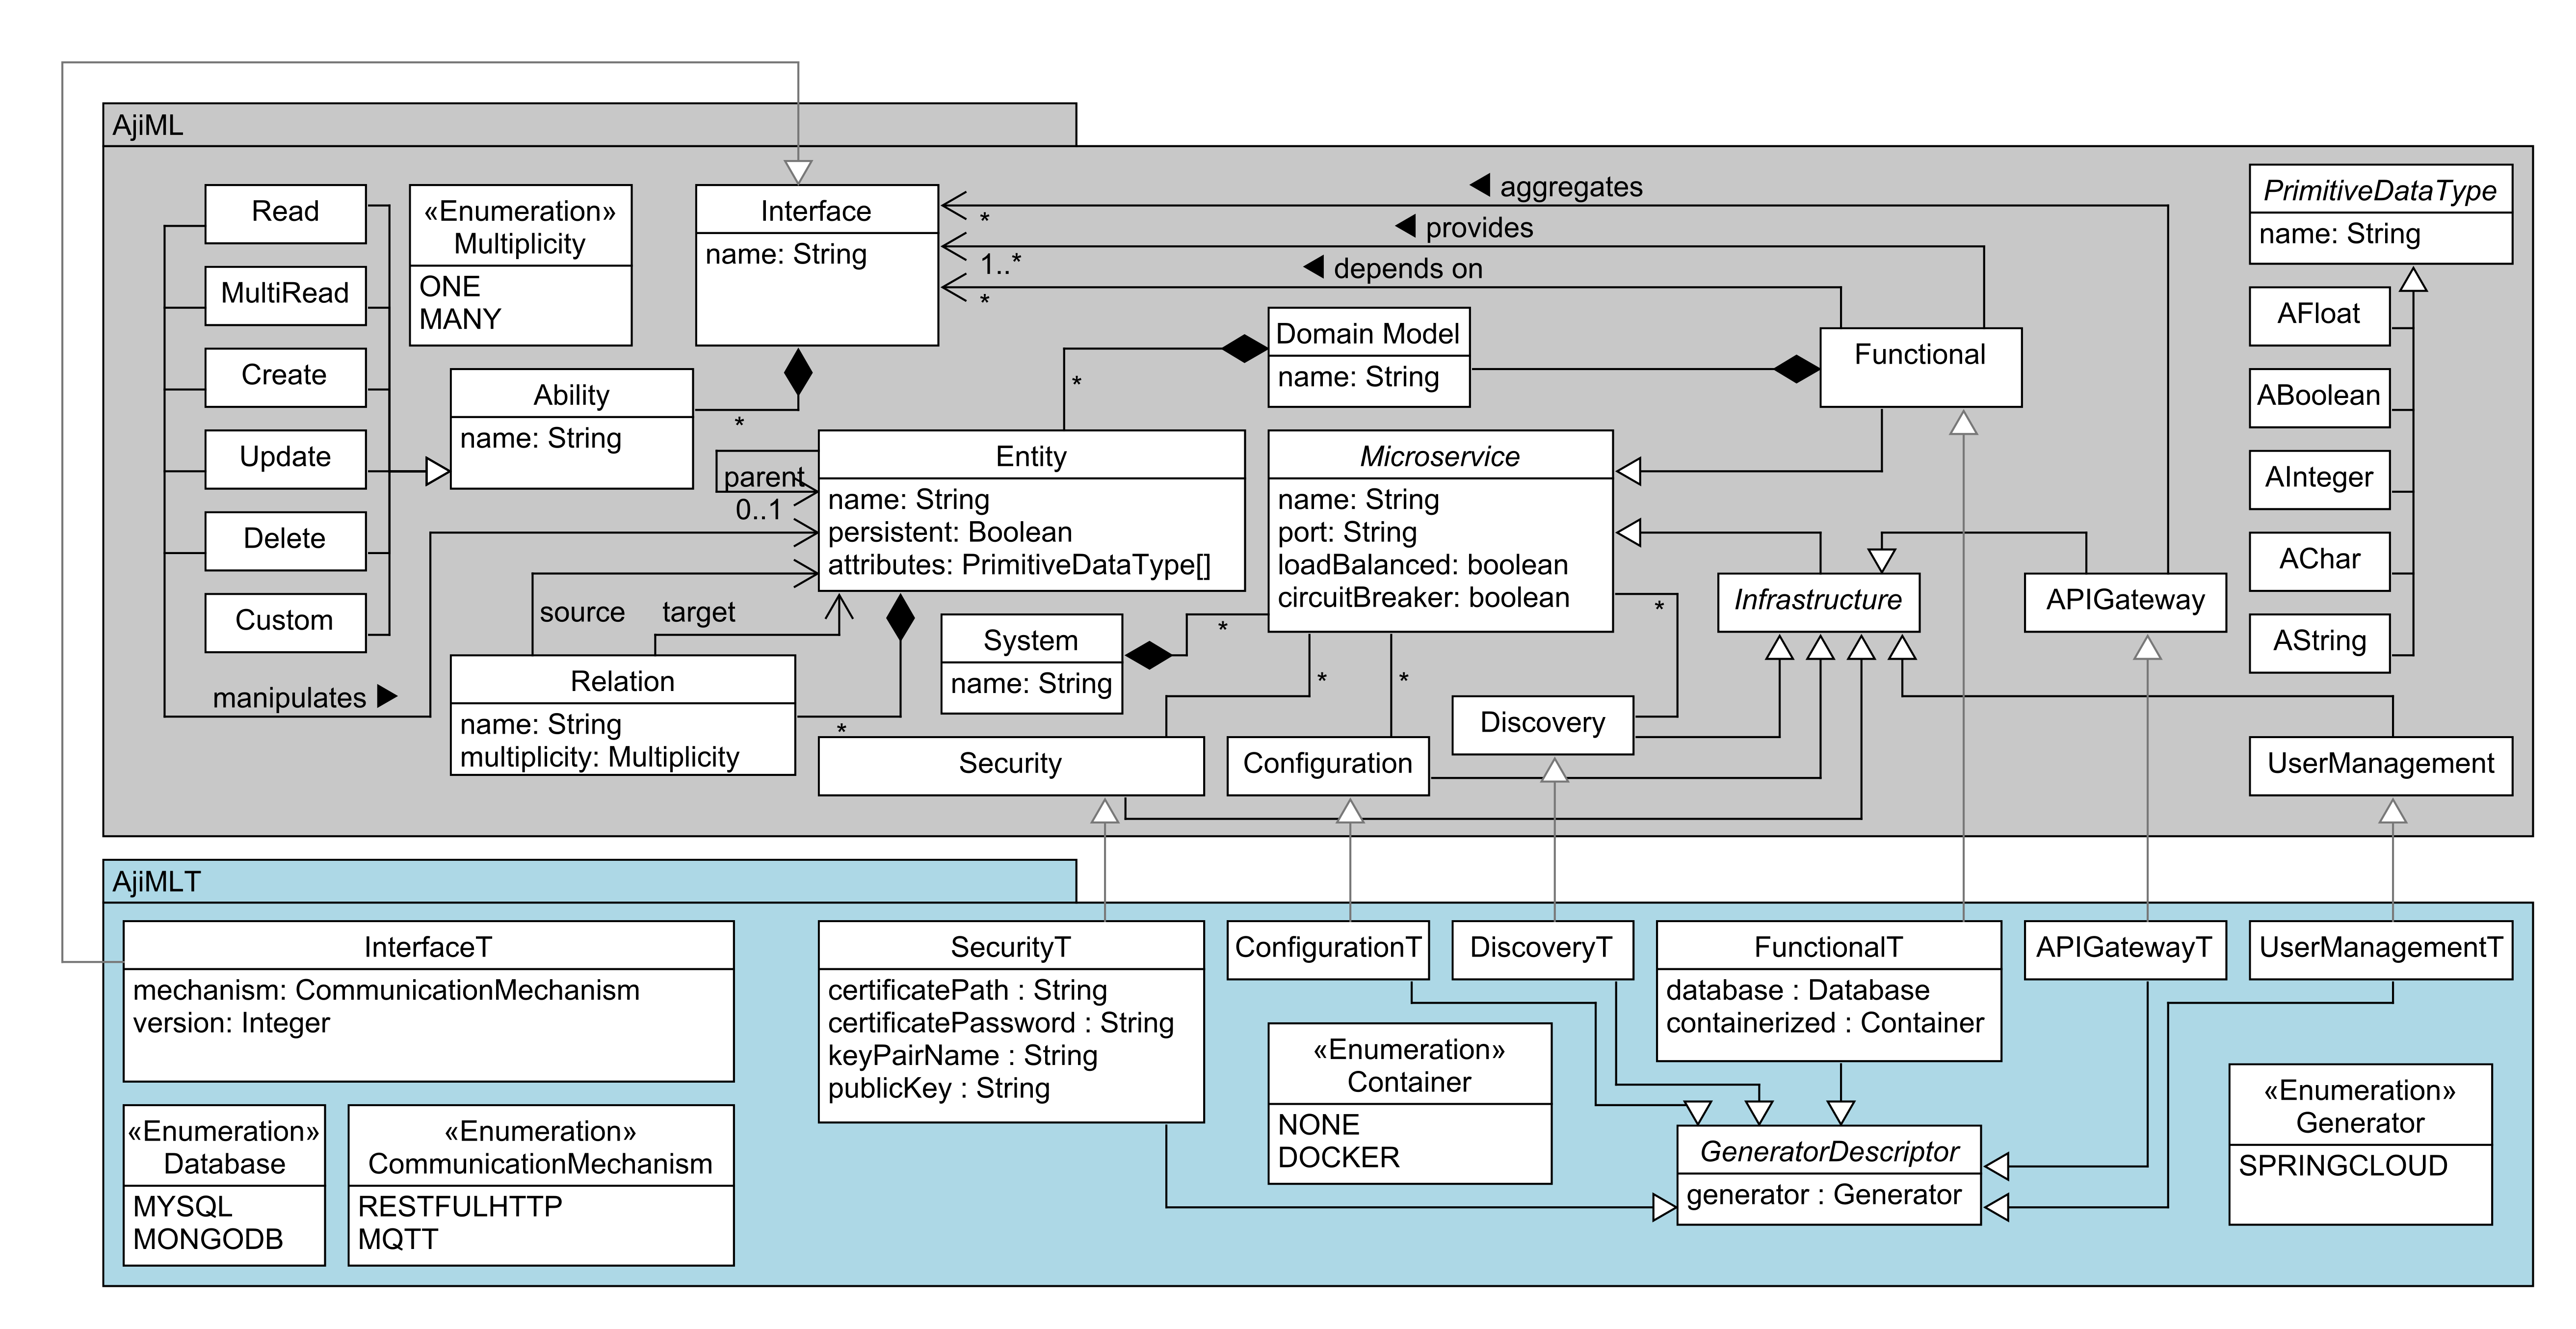
\includegraphics[width=\textwidth]{bilder/k3/k3_ajil.png}
\caption[Das AjiL Metamodell]{Das AjiL Metamodell \cite{ajilGithub}}
\end{figure}

AjiL bildet in seinem Metamodell verschiedene Aspekte von Microservice-Architekturen ab: So existieren Domain Models und Entities, welche Fachlichkeiten abbilden. Klassen wie Microservice, Security, Configuration oder Discovery bilden die technischen Metaklassen ab. Ebenso existieren Infrastruktur-Klassen wie Database oder Container. Das AjiMLT-Paket des Metamodells bildet konkrete Typen ab. So existiert beispielsweise ein Enum, welcher die Kommunikation einer Schnittstelle spezifiziert, konkret REST oder das Messaging-Protokoll MQTT.

Das AjiL-Metamodell bildet einen recht breiten Bereich der Microservice-Entwicklung ab, jedoch gibt es auch einige fehlende Abstraktionen, wie solche, die das Domain-Driven Design abbilden oder konkretere Cloud-Architekturen. AjiL setzt vieles davon implizit in den Generierungstemplates um, ohne explizite Modellklassen. Dadurch entsteht eine hohe Inflexibilität durch starre Teile des Templates.

Auch wenn AjiL einige interessante Ansätze bietet, auf denen man aufbauen kann, wie dessen Ansatz zum Schnittstellenmanagement und den ähnlichen Anforderungen an die zu generierenden Anwendungen, ist AjiL keine hinreichende Lösung, um DDD abzubilden und deploybare Anwendungen zu generieren.

\newpage

\subsubsection{Context Mapper}

\begin{figure}[ht]
\centering
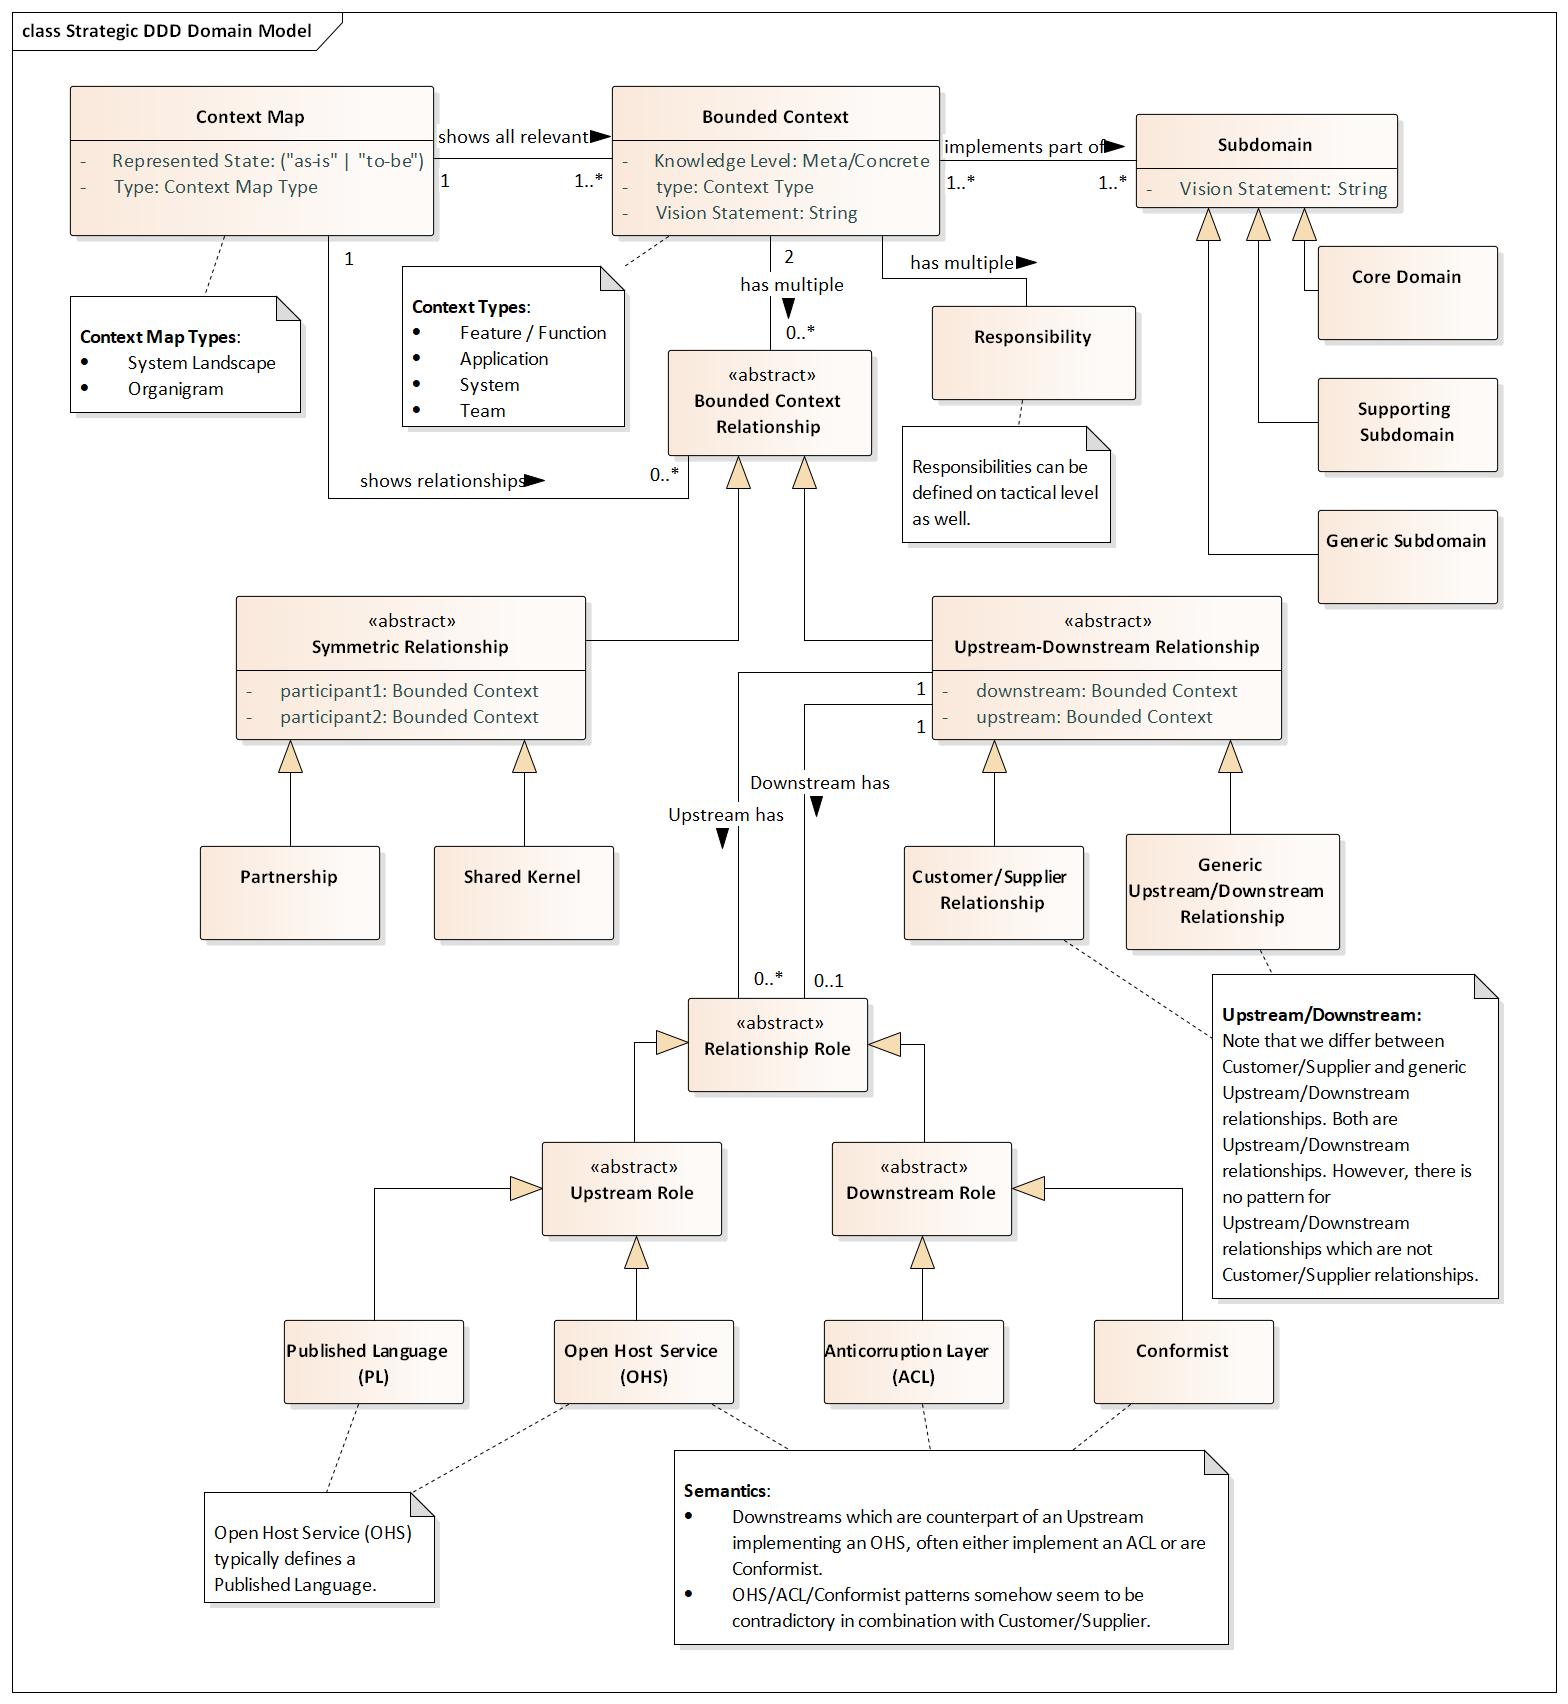
\includegraphics[height=15cm]{bilder/k3/k3_context_mapper.png}
\caption[Das Context Mapper Metamodell]{Das Context Mapper Metamodell \cite[S.3]{mapper}}
\end{figure}

Context Mapper definiert ein sehr umfassendes Metamodell, welches die Konzepte des DDD in höchster Ausführlichkeit modelliert. Context Mapper nutzt dieses, um Context Maps von Domänen zu generieren. Dementsprechend ist die Technologie keine Lösung, um Microservice-Anwendungen zu generieren. Jedoch ist die Modellierung eine umfassende Grundlage für eine Metamodellschicht, die das Strategic Design des DDD abbildet. Eine exakte Wiederverwendung bietet sich aus Gründen der Übersichtlichkeit nicht an, da Context Mapper so umfassend modelliert, dass eine auf generierende Anwendungen fokussierte Modellierung auch mit weniger Metamodell-Klassen auskommen kann. So ist beispielsweise die explizite Modellierung von Responsibilities oder Subdomains für zu generierende Microservices nicht notwendig. Aspekte der Visualisierung hingegen eignen sich sehr gut, um in einem dem Ziel dieser Arbeit angepassten Rahmen aufgegriffen zu werden.

\subsubsection{OCCI}

\begin{figure}[ht]
\centering
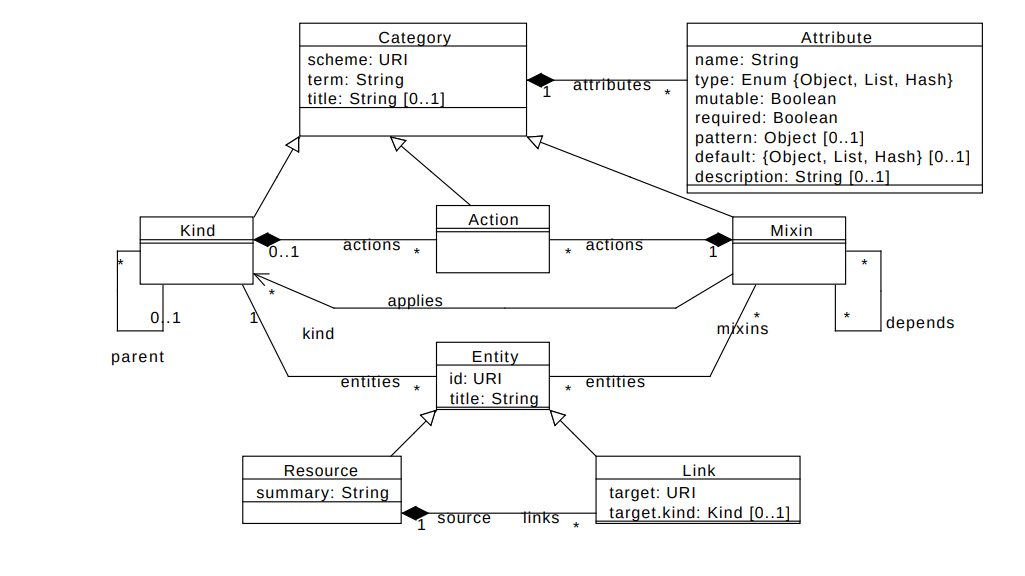
\includegraphics[width=\textwidth]{bilder/k3/k3_occi.png}
\caption[Das OCCI Metamodell]{Das OCCI Metamodell \cite[S.5]{edmonds}}
\end{figure}

Das Metamodell des Open Cloud Computing Interface (OCCI) stellt eine kompakte Abstraktion dar, um Cloud-Ressourcen und -Dienste effektiv zu modellieren. Es vermeidet eine direkte Abstraktion von spezifischen Konzepten wie Container oder Deployments. Stattdessen verwendet OCCI allgemeinere Klassen wie Entity, Resource und Link, um eine breite Palette von Cloud-Konzepten und Beziehungen darzustellen.

Beispielsweise kann eine Entity in diesem Modell einen konkreten Cloud-Service oder eine virtuelle Maschine repräsentieren, während Resource für spezifische Dienste wie Speicherplatz oder Rechenkapazitäten steht. Link kann genutzt werden, um die Verbindungen zwischen verschiedenen Ressourcen oder Diensten abzubilden, wie etwa die Zuordnung eines Netzwerkdienstes zu einem bestimmten Container. Dieser abstrakte Ansatz ermöglicht es, das Modell flexibel und anpassbar für eine Vielzahl von spezifischen Cloud-Umgebungen und Anwendungsfällen zu gestalten.

Trotz der Fähigkeit der Technologie, Cloud-Infrastrukturen umfassend zu modellieren und zu generieren, ist sie für die Anforderungen dieser Arbeit aufgrund ihrer komplexen Handhabung und der Fokussierung auf Infrastruktur anstatt auf Anwendungssoftware weniger geeignet. 

\begin{figure}[ht]
\centering
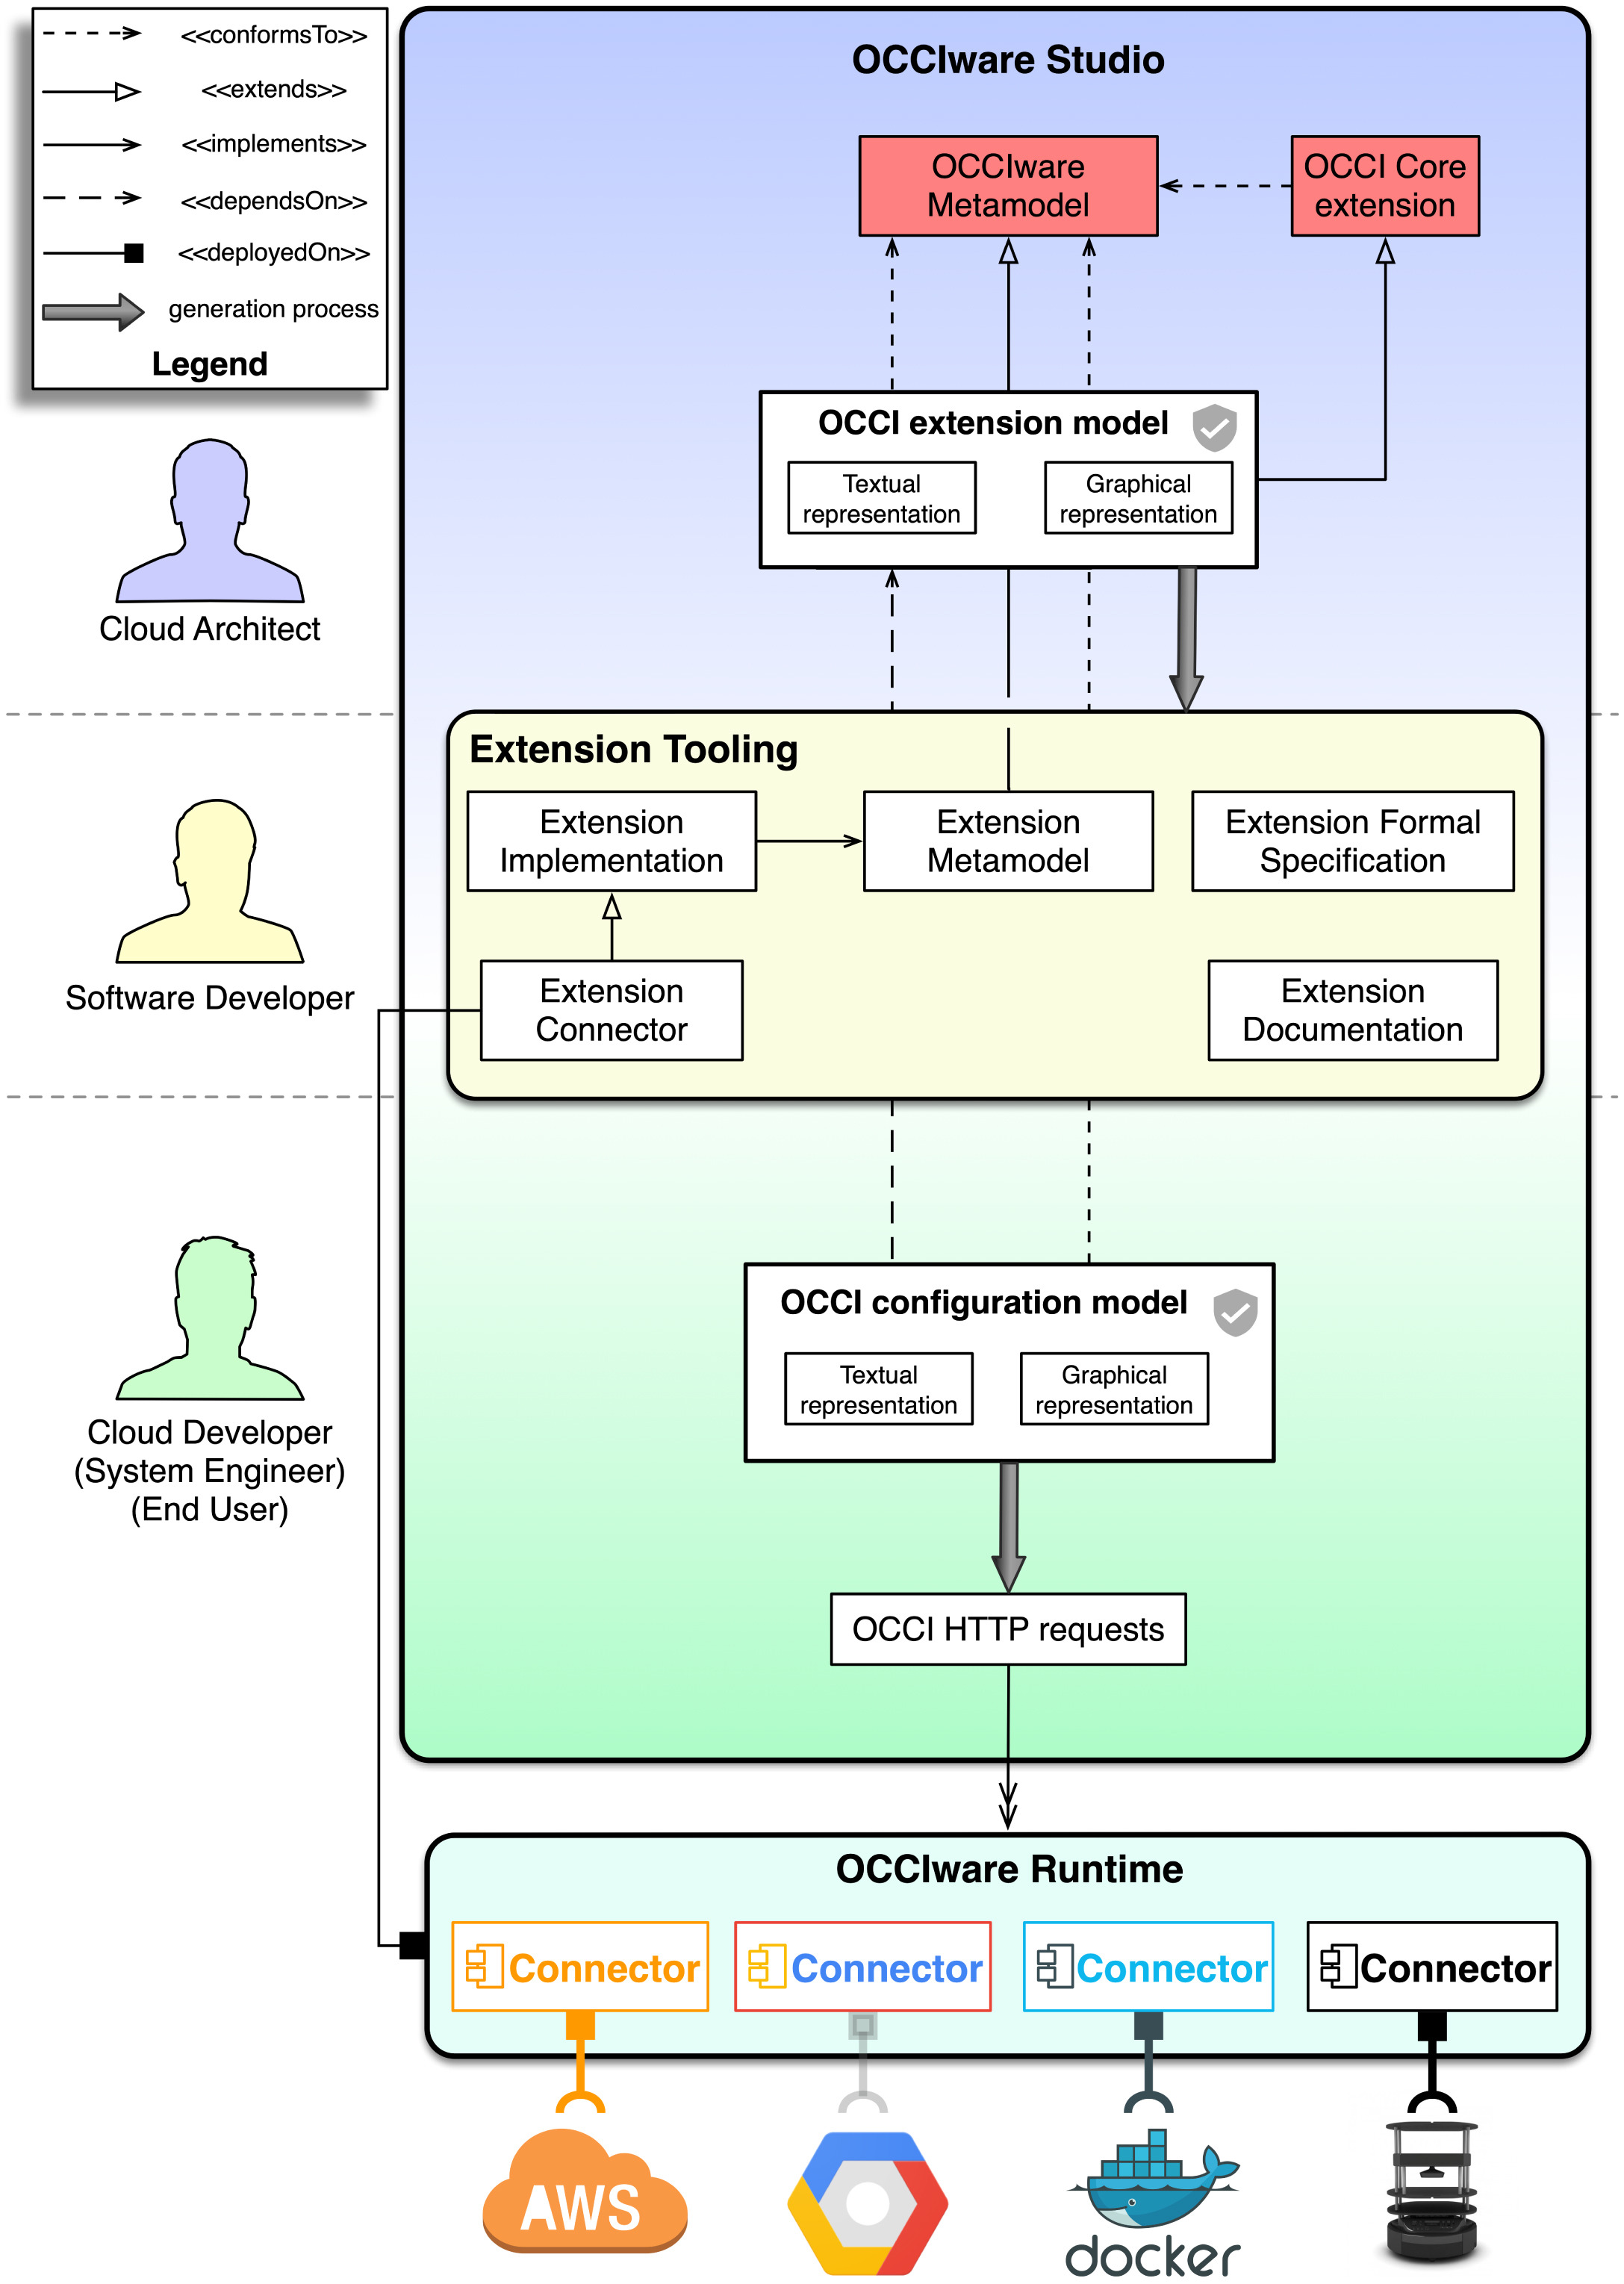
\includegraphics[height=12cm]{bilder/k3/k3_occi_2.jpg}
\caption[OCCIware Anwendungsumgebung]{Das OCCI Metamodell als Teil der komplexen OCCIware Anwendungsumgebung \cite{zalila}}
\end{figure}

\newpage


\subsubsection{ARGON}

Die Technologie ARGON strukturiert den Ansatz, Cloud-Infrastrukturen modellbasiert zu entwickeln, in mehrere Ebenen. Im Gegensatz zu OCCI, das ein umfangreiches Anwendungsframework bietet, konzentriert sich ARGON auf die Definition eines plattformunabhängigen Metamodells (PIM) sowie spezifischer Metamodelle (PSM) für AWS und Microsoft Azure. Mittels M2M-Transformationen ist eine gegenseitige Umwandlung möglich. Zudem sind M2T-Transformationen vorgesehen, um Infrastructure-as-Code mittels Ansible oder Terraform zu erzeugen.

In diesem Kontext erweist sich ARGON als deutlich geeigneter als OCCI, da es sich auf die praxisnahe Erstellung von Software-Komponenten konzentriert, die durch ein konkreteres Metamodell definiert werden, anstatt auf einen abstrakten, plattformübergreifenden Cloud-Baukasten. Auch der hierarchische Ansatz und das in Relation setzen von Cloud-spezifischen Modellen sind sinnvoll aufgreifbare Konzepte.
Die Problematik der fehlenden Anwendungsebene liegt jedoch weiterhin vor. Die Entwicklung einer Schnittstelle zu ARGON wäre eine Möglichkeit, diese zu lösen.

Stattdessen soll im Rahmen dieser Arbeit, gemäß dem Fokus auf das lauffähige Deployment von Microservice-Architekturen, eine Lösung entwickelt werden, die Anwendungsmodellierung und Deployment für eine konkrete Zielplattform in einem Metamodell vereint. Dabei kann der ARGON-Ansatz plattformunabhängige Modellelementen und spezifischer Modellelemente zu modellieren integriert werden. 

\begin{figure}[ht]
\centering
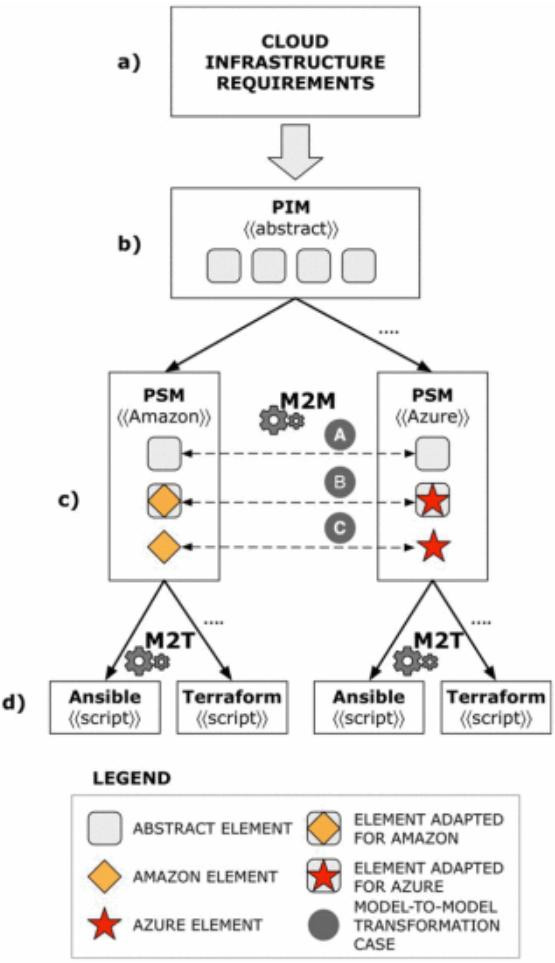
\includegraphics[height=11cm]{bilder/k3/k3_argon.jpg}
\caption[Architekturkonzept von ARGON]{Architekturkonzept von ARGON \cite{argon}}
\end{figure}

\subsection{Auswahl der Technologie}

Die Umsetzung des Metamodells erfolgt mit dem Eclipse Modeling Framework (Abk.: EMF), einem quelloffenen Java-Framework. Weiterhin kommen die ebenfalls quelloffenen Frameworks Eclipse Sirius, das die Visualisierung von Modellen ermöglicht, und Acceleo, das aus EMF-Modellen Code generieren kann, zum Einsatz. Diese stehen Eclipse als Plugins zur Verfügung. Die generierten Anwendungen sollen die Programmiersprache Java verwenden. Zudem wird das Spring Framework eingesetzt, welches die Implementierung verschiedenster Strukturen vereinfacht. Als Technologie zur Umsetzung von eventgetriebener Architektur wird Apache Kafka verwendet. Die generierten Applikationen sollen mittels Gradle gebaut und als Docker Image ausgeführt werden können. Als Cloud-Infrastruktur wird die Google Cloud gewählt, in welcher die Anwendungen auf einem Kubernetes-Cluster laufen sollen. Mit der Unix-Shell Bash werden dazu nötige Skripte umgesetzt. Als Datenbank Technologie wird die in-memory Datenbank H2 verwendet.


%%%%%%%%%%%%%%%%%%%%%%%%%%%%%%%%%%%%%%%%%%%%%%%%%%%%%%%%%%%%%%%%%%%%%%%%%%%%%%%%%%%%%%%%%%%%%%%%%%%%%%%%%%%%%%%%%%%%
%			DSL
%%%%%%%%%%%%%%%%%%%%%%%%%%%%%%%%%%%%%%%%%%%%%%%%%%%%%%%%%%%%%%%%%%%%%%%%%%%%%%%%%%%%%%%%%%%%%%%%%%%%%%%%%%%%%%%%%%%%

\newpage
\section{Entwicklung der eigenen DSL}

\subsubsection{Grundkonzept - Definition verschiedener Modellschichten}

Um ein Metamodell für Microservice-Architekturen zu konzipieren, wird zunächst ein plausibles, konkretes Modell betrachtet. Basierend auf einer Analyse dieses Modells soll beginnend ein grundlegender Ansatz gewählt werden, der im Kontext einer Abstraktion sinnvoll erscheint.

Hierzu wird ein Beispielmodell (Abbildung 4.6) eingeführt, das eine Domäne umfasst. Diese besteht aus den Kontexten Customer und Marketing, die eine Customer/Supplier-Beziehung haben. Weiterhin gibt es Microservices zu diesen Kontexten, die über eine Schnittstelle miteinander kommunizieren. Die Ausführungsumgebung wird mit spezifischer Servicekonfiguration und einem Modellelement, das die Cloud-Umgebung beschreibt – hier die Google Cloud-Infrastruktur – ebenfalls modelliert.

Bei der Betrachtung wird folgendes festgestellt: Die existierenden Modellelemente lassen sich in fachliche Elemente, technische Elemente oder Infrastrukturelemente gruppieren. Diese Gruppierung wird als gemeinsame Schicht definiert. Innerhalb ihrer Schicht haben die Elemente Beziehungen zu anderen Modellelementen derselben Schicht. Weiterhin können Beziehungen existieren, die über diese Schichten hinausgehen, das heißt, es gibt Abbildungen von Elementen einer Schicht auf Elemente anderer Schichten.

Da durch Schichten die mögliche Komplexität besser gegliedert und somit einfacher handhabbar gemacht wird, wird das Metamodell ebenfalls schichtbasiert konzipiert. Neben der Zuordnung der Konzepte in die passende Schicht muss dabei erforscht werden, wie die Beziehungen innerhalb und zwischen den Schichten umgesetzt werden können. Nach abschließender Betrachtung aller Schichten muss das Metamodell im Kontext der Konzeption von Codegenerierung und Migrationsfähigkeiten weiterhin iterativ überprüft und gegebenenfalls nachgebessert werden. Hierbei werden die Bewertungskriterien aus den einleitenden Überlegungen berücksichtigt.

\begin{figure}[ht]
\centering
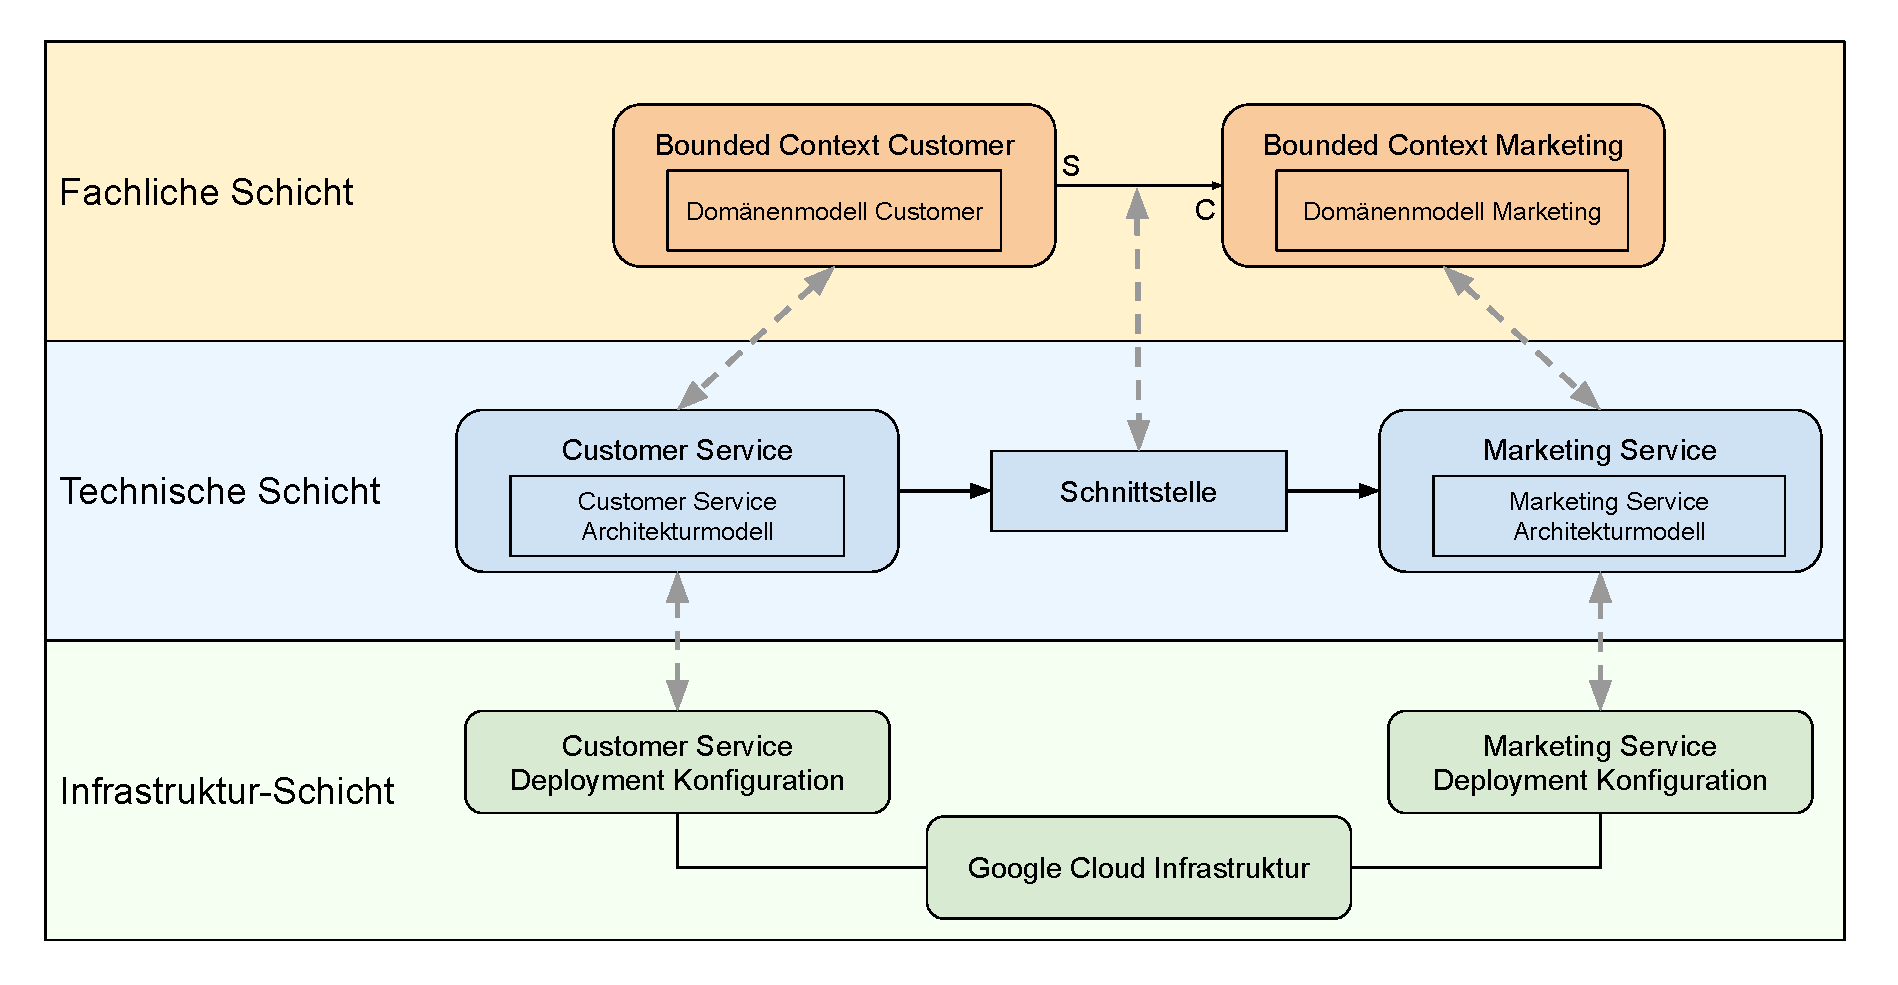
\includegraphics[width=0.8\textwidth]{bilder/k3/konzept.pdf}
\caption[Erkennbare Schichten in einem Modell einer Microservice-Architektur]{Erkennbare Schichten in einem Modell einer Microservice-Architektur}
\end{figure}

%%%%%%%%%%%%%%%%%%%%%%%%%%%%%%%%%%%%%%%%%%%%%%%%%%%%%%%%%%%%%%%%%%%%%%%%%%%%%%%%%%%%%%%%%%%%%%%%%%%%%%%%%%%%%%%%%%%%
%			Fachl. MDD
%%%%%%%%%%%%%%%%%%%%%%%%%%%%%%%%%%%%%%%%%%%%%%%%%%%%%%%%%%%%%%%%%%%%%%%%%%%%%%%%%%%%%%%%%%%%%%%%%%%%%%%%%%%%%%%%%%%%

\subsection{Modellierung des Model-Driven Designs}

Beginnend wird das DDD in das Metamodell integriert. Dieses findet sich in einer Klasse für die fachlichen Schicht, der \glqq DomainModelLayer\grqq{}, wieder. Die Schicht besteht aus drei Abstraktionsebenen: dem Domänenmodell, dem MDD und dem Strategic Design. Im Folgenden werden diese farblich unterschieden und die detailliertere Konzeption ausgeführt. Zur besseren Übersicht werden dabei bereits eingeführte Klassen und Relationen nach Möglichkeit ausgeblendet.

\begin{figure}[ht]
\centering
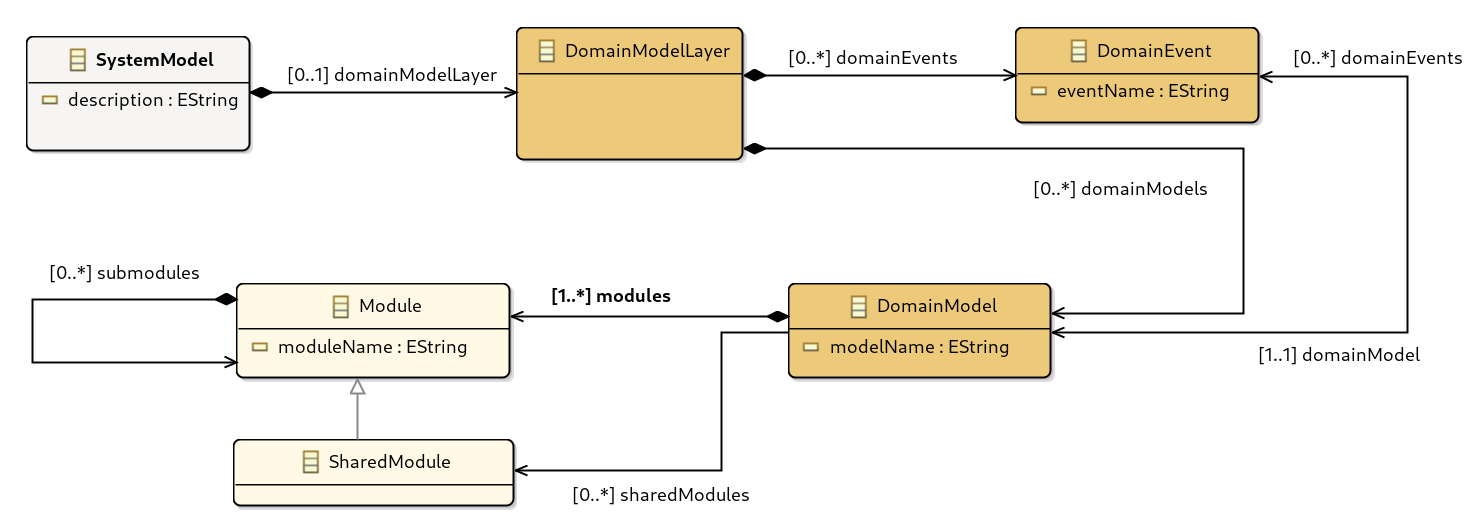
\includegraphics[width=\textwidth]{bilder/k4/1.png}
\caption[Metamodell - Fokus: Fachliche Schicht, Domänenmodelle und Pakete]{Metamodell - Fokus: Fachliche Schicht, Domänenmodelle und Pakete}
\end{figure}

Die fachliche Schicht besteht aus beliebig vielen benannten \glqq DomainModels\grqq{}. Weiterhin enthält diese ebenfalls beliebig viele \glqq DomainEvents\grqq{}. Durch eine bidirektionale Assoziation kann die Referenz von einem DomainModel zu verschiedenen Events beschrieben werden. Die Events selbst sind dabei nur einem DomainModel zugeordnet. Ein hypothetisches Event, das in mehreren Domänenmodellen vorkommt, wäre in dem Analyseprozess einer Problemdomäne ein Indiz für ein nicht erkanntes Domänenmodell.

Das DomainModel besitzt weiterhin Module, umgesetzt mit einer Klasse \glqq Module\grqq{}, welche wiederum Submodule enthalten können. Es zeigte sich während der Konzeption, dass es vorteilhaft ist, dass jedes DomainModel mindestens ein Modul besitzen muss. Diese Entscheidung erleichtert einerseits eine strukturiertere Codegenerierung. Andererseits wird dadurch eine deutlich einfachere Besitzbeziehung für das noch einzuführende \glqq ModelElement\grqq{} realisiert. Auch der Aufwand für die  Konzeption der dazugehörigen konkreten Syntax sinkt bedeutend. Die von Module abgeleitete Klasse \glqq SharedModule\grqq{} beschreibt Module, die in mehreren DomainModels vorkommen können. Diese Modellierung ist notwendig, um eine korrekte Umsetzung des noch einzuführenden Konzepts Shared Kernel zu ermöglichen.

\newpage

\begin{figure}[ht]
\centering
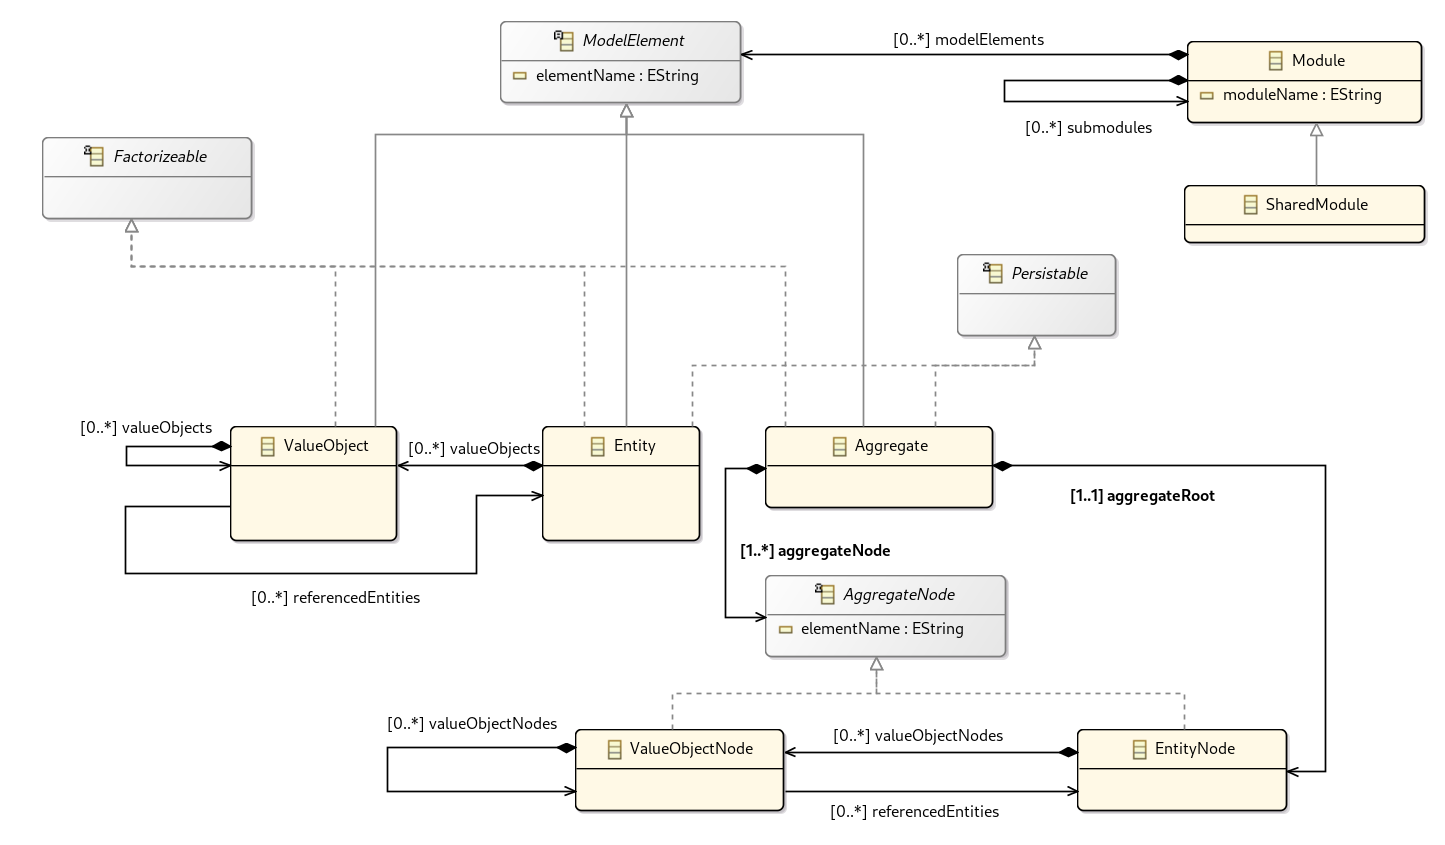
\includegraphics[width=\textwidth]{bilder/k4/2.png}
\caption{Metamodell - Fokus: Entitiy, Value Object und Aggregate}
\end{figure}

Als abstrakte Basisklasse des MDD wird das ModelElement entworfen, welches in Module beliebig oft enthalten sein kann. Davon lassen sich die aus dem MDD bekannten Konzepte der Entities, Value Objects und Aggregates als Klassen ableiten. Nach dem DDD sind diese von Factories erzeugbare Objekte, umgesetzt durch die Einführung einer Schnittstelle namens \glqq Factorizable\grqq{}. Dies wurde symmetrisch für Entities und Aggregates mit der Schnittstelle \glqq Persistable\grqq{} umgesetzt. Die Besitz- und Referenzrelation für Value Objects und Entities ist ebenso eine direkte Umsetzung der Definition des DDD.

Die modellgetreue Definition des Aggregates gestaltet sich schwierig. Die Umsetzung einer von außen zugreifbaren Entity-Wurzel mit von außen nicht zugreifbaren Blättern, welche Entities oder Value Objects sind, mit denselben Relationen, die aber nur untereinander gelten, hat sich als nicht elegant umsetzbar erwiesen. Der Versuch, eine einzige Entity-Klasse im Modell abzubilden, führte dazu, dass Elemente, die eigentlich vom Aggregate abgekapselt sein sollten, Zugriff darauf erhalten könnten. Diese Kapselung von Beziehungen muss durch eigene Klassen für Entities und Value Objects in einem Aggregate realisiert werden. Dementsprechend wird eine Klasse \glqq EntityNode\grqq{}, die einmalig als Wurzel existieren muss, modeliert. Weiterhin wird dazu eine abstrakte Klasse \glqq AggregateNode\grqq{}, und die diese ableitenden Klassen \glqq EntityNode\grqq{} und \glqq ValueObjectNode\grqq{} eingeführt.

\newpage


\begin{figure}[ht]
\centering
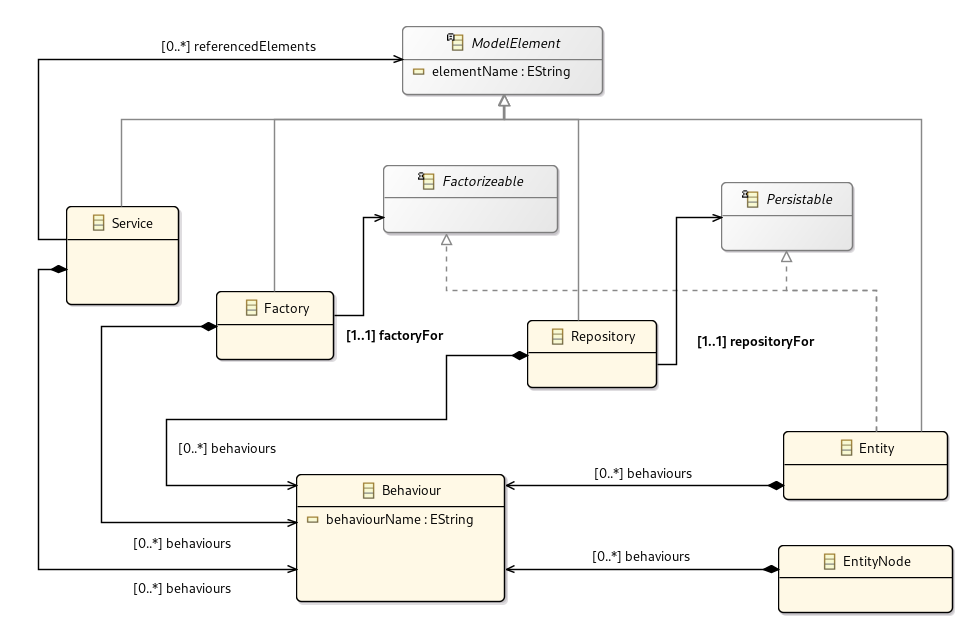
\includegraphics[width=\textwidth]{bilder/k4/3.png}
\caption{Metamodell - Fokus: Service, Repository, Factory und Behaviour}
\end{figure}

Es werden zu den MDD-Konzepten passenden Klassen \glqq Service\grqq{}, \glqq Factory\grqq{} und \glqq Repository\grqq{}, welche ebenfalls Ableitungen von ModelElement sind, konzipiert. Die bereits eingeführten Schnittstellen Factorizeable und Persistable werden von Factory und Repository passend referenziert. Dabei sind sowohl Factory als auch Repository je Objekt ihrer Klasse nur maximal einem, die Schnittstelle implementierenden, Objekt zugewiesen. Die Klasse Service hat weiterhin eine Assoziation zu beliebig vielen ModelElements, mit dem Zweck, Anwendungslogik umsetzen zu können. Eine Klasse Behaviour wird weiterhin zusätzlich eingeführt. Dies zeigte sich als notwendig, um das Verhalten in der Generierung und Modellierung präzise beschreiben zu können.


%%%%%%%%%%%%%%%%%%%%%%%%%%%%%%%%%%%%%%%%%%%%%%%%%%%%%%%%%%%%%%%%%%%%%%%%%%%%%%%%%%%%%%%%%%%%%%%%%%%%%%%%%%%%%%%%%%%%
%			Fachl. Strategic Design
%%%%%%%%%%%%%%%%%%%%%%%%%%%%%%%%%%%%%%%%%%%%%%%%%%%%%%%%%%%%%%%%%%%%%%%%%%%%%%%%%%%%%%%%%%%%%%%%%%%%%%%%%%%%%%%%%%%%
\newpage
\subsection{Modellierung des Strategic Designs}

\begin{figure}[ht]
\centering
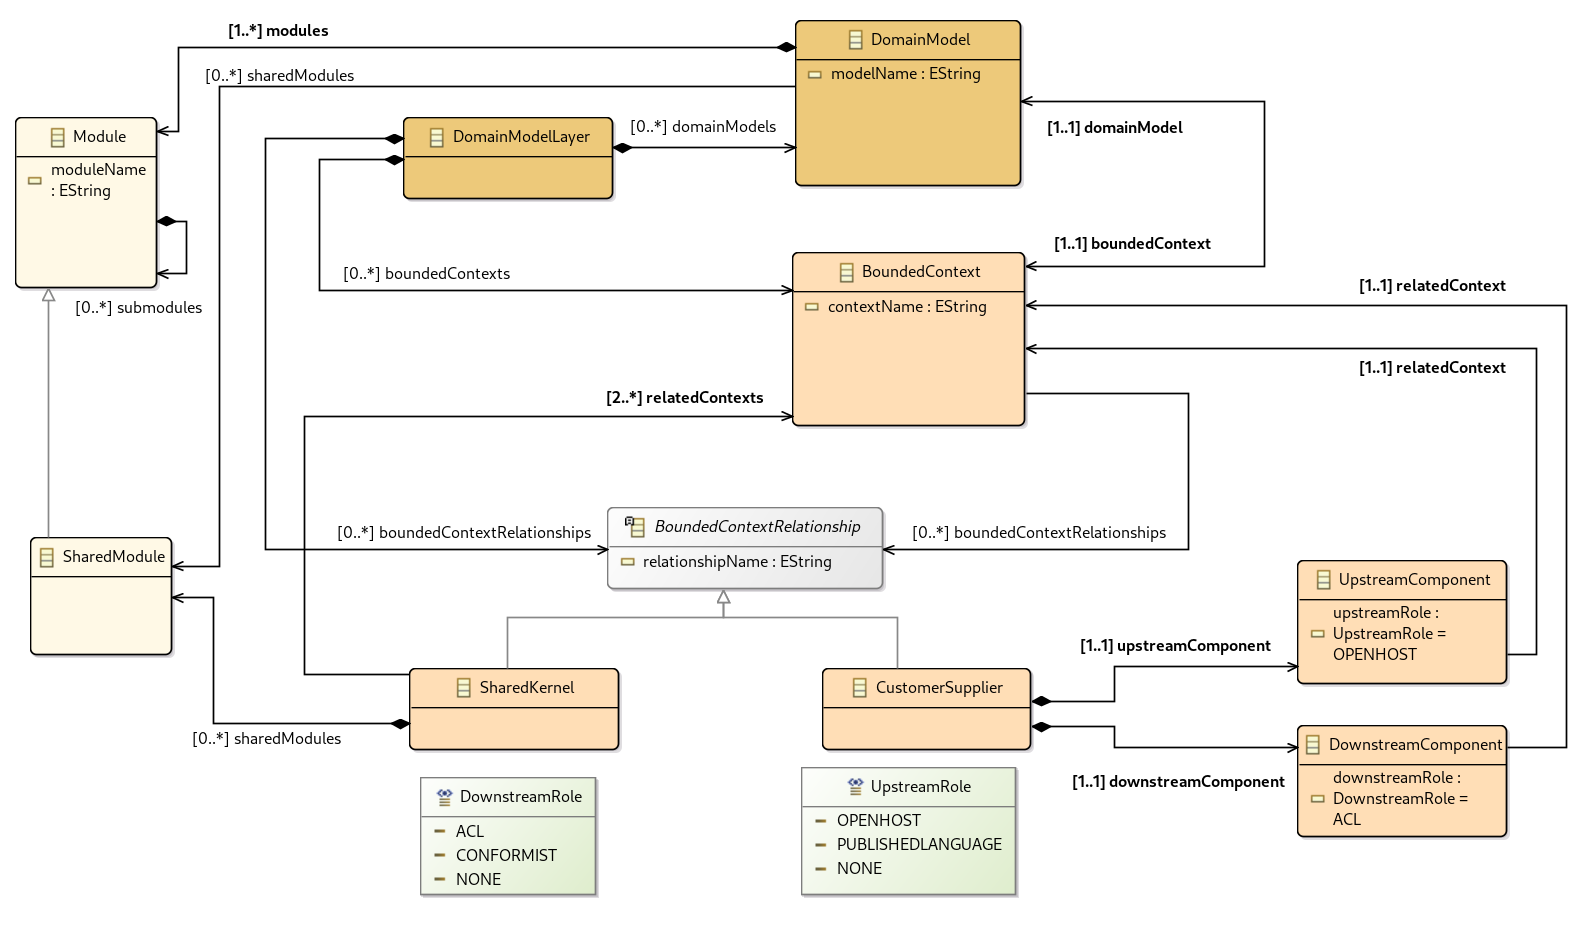
\includegraphics[width=\textwidth]{bilder/k4/4.png}
\caption{Metamodell - Fokus: Strategic Design}
\end{figure}

Die Modellierung des Bounded Context im Metamodell beginnt mit der Zuweisung der zugehörigen Klasse \glqq BoundedContext\grqq{} als Teil des DomainModelLayer. Weiterhin wird nach dem DDD eine Ist-Beziehung zwischen DomainModel und BoundedContext eingeführt. In Betrachtung des Strategic Design soll der Bounded Context explizit vom DomainModel unterscheidbar sein, da im Folgenden die Beziehungen dieser untereinander im Vordergrund stehen, während das DomainModel den Blick in den Bounded Context symbolisiert. Ebenso Teil des DomainModelLayer ist die abstrakte Klasse \glqq BoundedContextRelationship\grqq, welche beliebig oft von einem Bounded Context referenziert werden kann. Diese beschreibt Beziehungen als eigene Objekte, analog zu dem Konzept von ContextMapper. \glqq SharedKernel\grqq{} und \glqq CustomerSupplier\grqq{} sind die zwei davon abgeleiteten Klassen. CustomerSupplier besitzt weiterhin jeweils eine sendende und empfangende Komponente, welche auf genau einen Bounded Context verweist. Im Gegensatz zu ContextMapper reicht hier eine reduzierte Modellierung der Konzepte des Strategic Design. Dies zeigte sich bei der Konzeption von Visualisierung und Generierung. Dabei ergab sich, dass die Modellierung der übrigen Strategic Design Konzepte als statische Enumerationen hinreichend ist. SharedKernel enthält außerdem noch die bereits erwähnte Referenz auf das SharedModule. Dies ist notwendig, um bei der Beschreibung des DomainModels dieses korrekt zu referenzieren. Das Fehlen kann somit zu einer unvollständigen Beschreibung führen, wodurch möglicherweise wichtige Aspekte zum Verständnis des Modells fehlen würden.


%%%%%%%%%%%%%%%%%%%%%%%%%%%%%%%%%%%%%%%%%%%%%%%%%%%%%%%%%%%%%%%%%%%%%%%%%%%%%%%%%%%%%%%%%%%%%%%%%%%%%%%%%%%%%%%%%%%%
%			Techn
%%%%%%%%%%%%%%%%%%%%%%%%%%%%%%%%%%%%%%%%%%%%%%%%%%%%%%%%%%%%%%%%%%%%%%%%%%%%%%%%%%%%%%%%%%%%%%%%%%%%%%%%%%%%%%%%%%%%

\newpage
\subsection{Modellierung der technischen Modellebene}

\begin{figure}[ht]
\centering
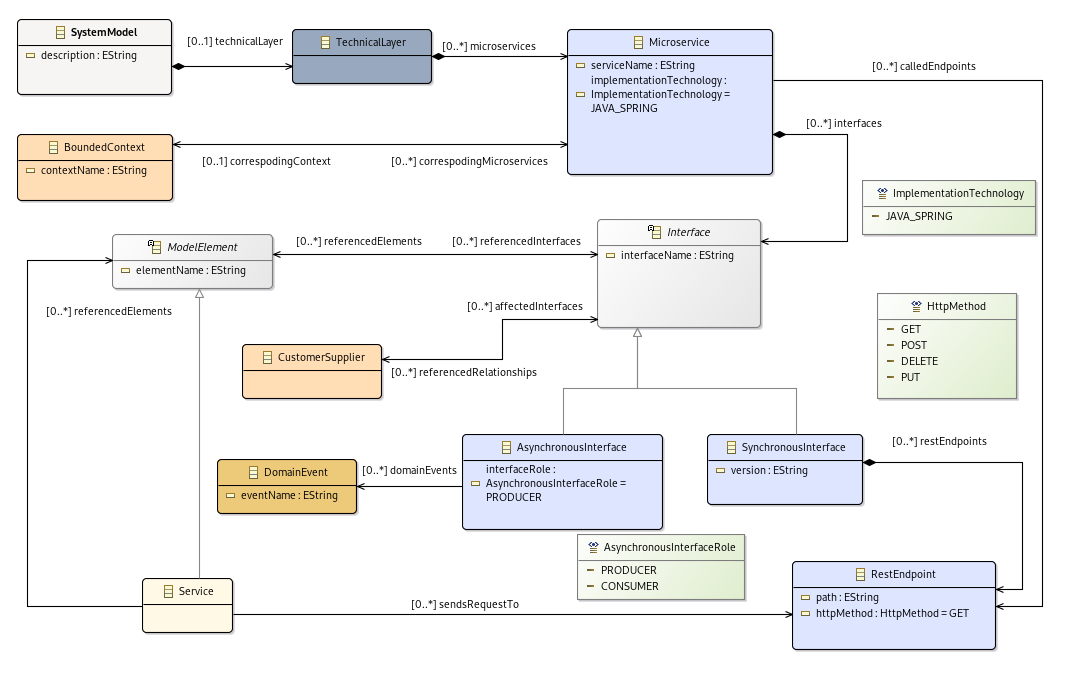
\includegraphics[width=\textwidth]{bilder/k4/5.png}
\caption{Metamodell - Fokus: Technische Schicht}
\end{figure}

Die technische Modellebene wird mit einer Klasse \glqq TechnicalLayer\grqq{} umgesetzt, welche die Microservices enthält. Die dazugehörige Klasse \glqq Microservice\grqq{} ist benannt und weiterhin mit einem Attribut vom Typ \glqq ImplementationTechnology\grqq{} versehen. Mögliche Implementierungstechnologien können so zukünftig hinzugefügt werden. Ein Objekt der Klasse Microservice besitzt beliebig viele \glqq Interfaces\grqq{}. Von dieser benannten abstrakten Klasse existieren weiterhin die Ableitungen \glqq AsynchronousInterface\grqq{} und \glqq SynchronousInterface\grqq{}. Asynchrone Schnittstellen sind dabei entweder Produzenten oder Konsumenten. Synchrone Schnittstellen sind demgegenüber versioniert und implementieren HTTP-Schnittstellen. Hier wird sich bewusst für eine Eingrenzung auf die Protokolle HTTP und das REST-Paradigma entschieden, da diese für synchrone Schnittstellen die relevantesten im Microservice-Kontext sind. Die zur synchronen Schnittstelle gehörigen REST-Endpunkte, modelliert durch eine Klasse \glqq RestEndpoint\grqq{}, besitzen einen Pfad sowie eine HTTP-Methode. Diese wird im dazugehörigen Enum spezifiziert. Bei der Konzeption der Implementierungsumsetzung der MDD-Bausteine wurde anfangs versucht, Gegenstücke zu diesen als eigenständige Klassen der technischen Schicht zu definieren. Jedoch stellte sich heraus, dass aufgrund des grundlegenden Konzepts des MDD, dem Erzeugen einer hohen Kohäsion zwischen Modellbausteinen und Umsetzung dieser, diese nicht zwingend benötigt werden. Dadurch hat eine Abwägung stattgefunden: Es wurde erwogen, ob aus Gründen der kognitiven Komplexität des Metamodells bestimmte Elemente explizit als Teil der Schicht definiert werden sollen.

Die alternative Überlegung war, ob auf diese Definition verzichtet werden sollte, obwohl Modellelemente in der technischen Abstraktionsebene implizit existieren. Entschieden wurde, auf die explizite Definition zu verzichten.

Die Klassen der technischen Schicht besitzen weiterhin verschiedene Assoziationen zu Klassen der fachlichen Schicht. So kann ein BoundedContext durch beliebig viele Microservices umgesetzt werden. Zwischen ModelElements und Interfaces können bidirektional beliebig viele Assoziationen existieren. Eine CustomerRelationship-Beziehung kann beliebig viele Schnittstellen betreffen. Ebenso kann eine Schnittstelle beliebig viele referenzieren. Dem AsynchronousInterface können verschiedene DomainEvents zugewiesen werden. Dies ist insbesondere im Prozess der Analyse der Problemdomäne eine wertvolle Assoziation.

Um den Zugriff auf REST-Endpunkte zu modellieren, wird einerseits eine Assoziation vom Microservice zum RestEndpoint eingeführt. Diese ist notwendig, um auf der Intermicroservice-Kommunikationsebene Architekturen zu entwerfen. Zusätzlich kann spezifiziert werden, wo im Service selbst ein Aufruf ausgelöst wird. Dafür wurde basierend auf dem MDD und somit der Richtlinie, Logik durch Services primär umzusetzen, dieses Aufrufen in der Klasse Service verortet.

%%%%%%%%%%%%%%%%%%%%%%%%%%%%%%%%%%%%%%%%%%%%%%%%%%%%%%%%%%%%%%%%%%%%%%%%%%%%%%%%%%%%%%%%%%%%%%%%%%%%%%%%%%%%%%%%%%%%
%			Infrastruktur
%%%%%%%%%%%%%%%%%%%%%%%%%%%%%%%%%%%%%%%%%%%%%%%%%%%%%%%%%%%%%%%%%%%%%%%%%%%%%%%%%%%%%%%%%%%%%%%%%%%%%%%%%%%%%%%%%%%%
\subsection{Modellierung der Infrastrukturellen Umgebung}

\begin{figure}[ht]
\centering
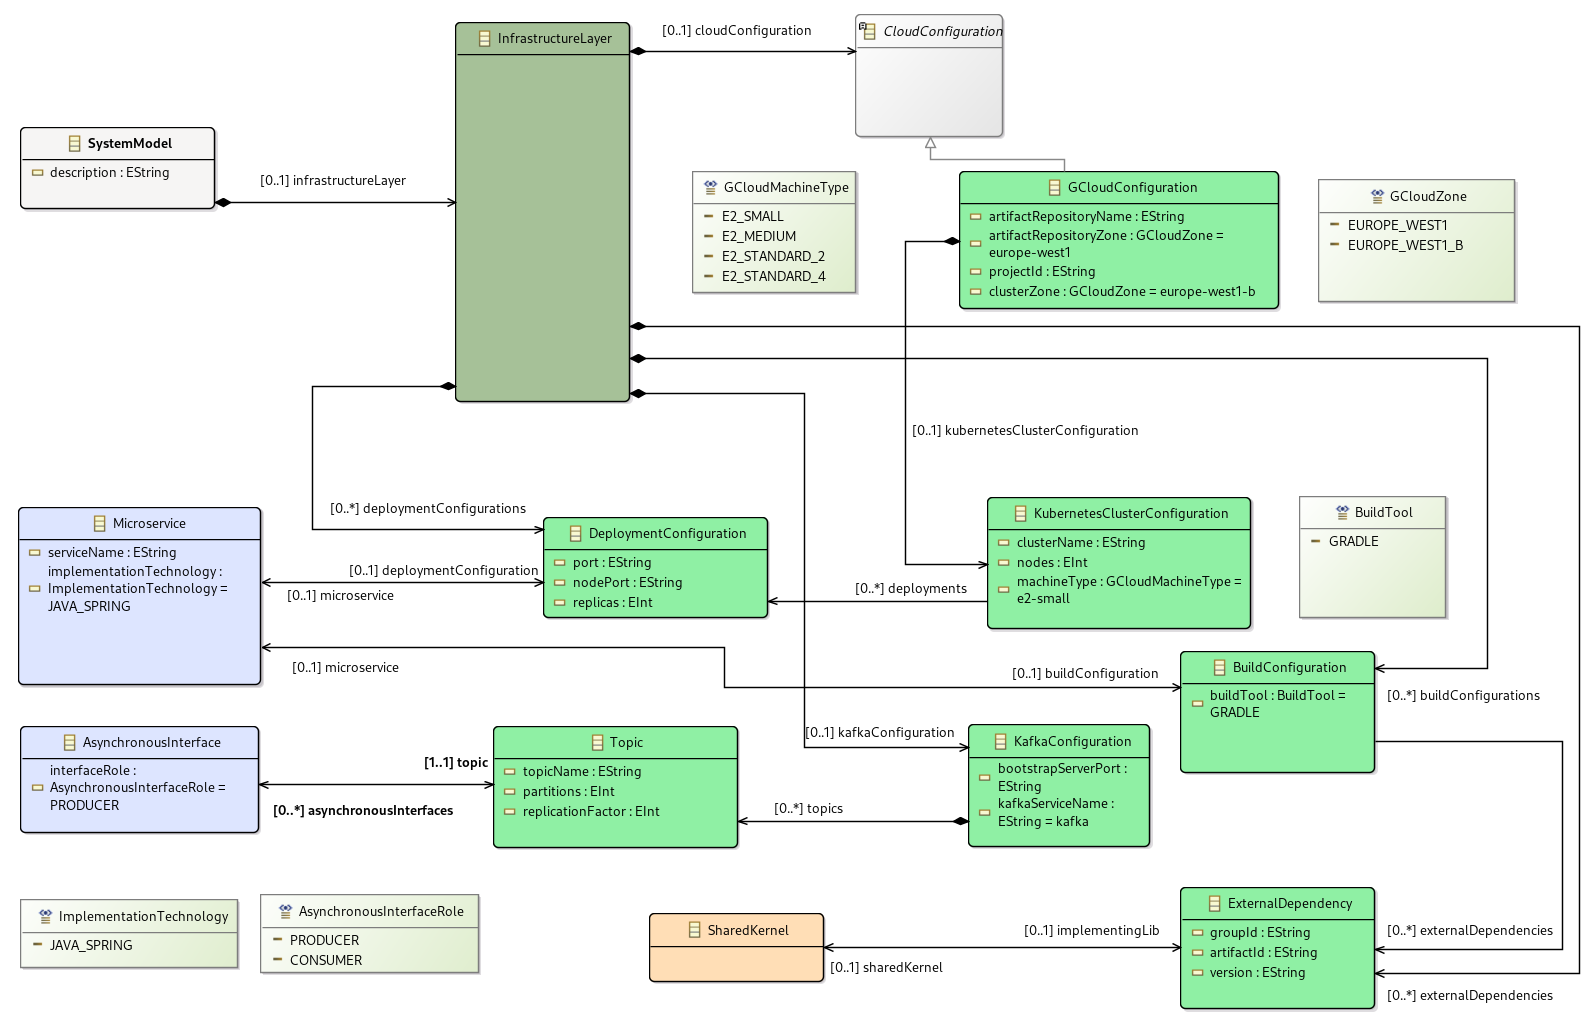
\includegraphics[width=\textwidth]{bilder/k4/6.png}
\caption{Metamodell - Fokus: Infrastrukturschicht}
\end{figure}

\newpage

Die Infrastrukturebene, umgesetzt durch die Klasse \glqq InfrastructureLayer\grqq{}, besitzt eine Konfiguration der Cloud-Umgebung. Diese wird als abstrakte Klasse \glqq CloudConfiguration\grqq{} entworfen, von der die \glqq GCloudConfiguration\grqq{} abgeleitet wird. Ergänzungen für AWS oder Azure würden dort ansetzen. Die GCloudConfiguration definiert GCP-spezifische, notwendige Eigenschaften. So definiert \glqq artifactRepositoryName\grqq{} und \glqq artifactRepositoryZone\grqq{} ein Ziel-Repository für Docker Images.

Das Attribut \glqq clusterZone\grqq{} definiert die Google-spezifische Region des Kubernetes-Clusters, welches durch die Klasse \glqq KubernetesClusterConfiguration\grqq{} modelliert wird. Diese wird außerdem als Teil der GCloudConfiguration modelliert. Bei der Kubernetes Konfiguration muss weiterhin bedacht werden, dass ein Kubernetes-Cluster Attribute besitzt, die unabhängig von dem Cloud-Anbieter sind. Jedoch gibt es auch welche die cloudspezifisch sind. Konkret wird hier noch ein Google-spezifischer Maschinentyp verwendet, welcher bei einer Erweiterung der Cloud Umgebungen abstrakter konzipiert werden müsste. Ebenso wird aktuell nur ein existierendes Cluster in der Cloud modelliert, da dies hinreichend für das Deployment einer Microservice-Architektur ist. Grundsätzlich möglich wären aber auch mehrere Cluster in einer Cloud-Umgebung.

Das Cluster referenziert weiterhin die Klasse \glqq DeploymentConfiguration\grqq{}. Diese beschreibt Deployment-Objekte in einem Kubernetes-Cluster. Modelliert werden diese als Teil der Infrastrukturschicht. Sie haben weiterhin eine bidirektionale Assoziation, welche Objekte der Klasse zu einem Microservice zuweisen können. Hier wurde darauf verzichtet das Konzept der Pods in das Metamodell mit aufzunehmen um die Komplexität zu reduzieren. Es wird daher festgelegt, dass jeder Service auf genau einem Pod, der genau einem Deployment zugewiesen ist, ausgeführt wird.

Symmetrisch zu der DeploymentConfiguration wurde die bidirektionale Assoziation für die Klasse \glqq BuildConfiguration\grqq{} und Microservice modelliert. Diese sind Teile der Infrastrukturschicht und gehen von einer Verwendung des Build-Tools Gradle aus. Andere Build-Tools wie z.B. Maven können in der dazugehörigen Enumeration \glqq BuildTool\grqq{} bei möglicher Erweiterung des Metamodells ergänzt werden. Die BuildConfiguration verweist auf die Klasse \glqq ExternalDependency\grqq, ebenfalls Teil des InfrastructureLayers. Diese besitzt eine auf das öffentliche Bibliotheksverzeichnis \glqq mvnrepository\grqq{} abgestimmte Attributierung. Eine weitere Relation zwischen ExternalDependency und SharedLib modelliert den Zusammenhang dieser.

Eine \glqq KafkaConfiguration\grqq{} definiert Port und Service-Name eines Kafka-Containers in der Cloud. Hier wurde sich gegen eine Abstraktion der asynchronen Kommunikationstechnologie entschieden, um die Komplexität des Metamodells nicht weiter zu erhöhen. Inwiefern eine Abstraktion verschiedener solcher Technologien überhaupt möglich wäre, wurde nicht näher betrachtet. Die KafkaConfiguration besitzt benannte Topics, welche von asynchronen Schnittstellen beschrieben oder konsumiert werden. Eine asynchrone Schnittstelle ist so modelliert, dass sie nur mit einem Topic interagiert. Weiterhin besitzt es die Attribute \glqq partitions\grqq{}, welches das Topic mit der angegebenen Zahl partitioniert, und \glqq replicationFactor\grqq{}, welches die Anzahl der Replikationen für Ausfälle definiert.


%%%%%%%%%%%%%%%%%%%%%%%%%%%%%%%%%%%%%%%%%%%%%%%%%%%%%%%%%%%%%%%%%%%%%%%%%%%%%%%%%%%%%%%%%%%%%%%%%%%%%%%%%%%%%%%%%%%%
%			Konkrete Syntax
%%%%%%%%%%%%%%%%%%%%%%%%%%%%%%%%%%%%%%%%%%%%%%%%%%%%%%%%%%%%%%%%%%%%%%%%%%%%%%%%%%%%%%%%%%%%%%%%%%%%%%%%%%%%%%%%%%%%
\newpage
\chapter{Entwicklung einer konkreten Syntax}

Mit Hilfe des Eclipse Modeling Frameworks und der Sirius-Erweiterung ist es möglich, spezifische Modelle zu konzeptionieren und zu visualisieren, die auf dem entwickelten Microservice-Metamodell basieren. Im Folgenden wird eine konkrete Syntax präsentiert und erörtert, wie diese erstellt wurde. Dabei wurde versucht, die Komplexität von Microservice-Architekturen durch verschiedene Modellsichten greifbarer zu machen, welche sich gegenseitig ergänzen.

Beginnend soll ein grundlegender, abstrakter Workflow skizziert werden, welcher die Modellierung einer Microservice-Architektur mit der DSL beschreibt. Dazu wird festgelegt, dass ein initiales Grundmodell vorhanden sein muss. Dieses muss alle notwendigen Wurzelklassen, wie zum Beispiel die Klasse \glqq System Model\grqq{}, beinhalten. Danach wird die Problemdomäne konzeptionell erfasst. Dies würde durch ein zuweisen der DDD-Konzepte, bzw. der Metamodellklassen der DomainModelLayer, umgesetzt werden. Dazu sollen im folgenden notwendige Darstellungen und Editoren entworfen werden. In einem nächsten Schritt, kann ein Modell mit einer technischen Schicht erweitert werden, welche die konkreten Dienste dazu modelliert. Abschließend soll eine dazu passende Infrastrukturschicht modelliert werden, die wiederum das bis zu diesem Schritt modellierte Modell ergänzt. Auch hierfür werden im folgenden Darstellungen und Editoren entworfen.

\begin{figure}[ht]
\centering
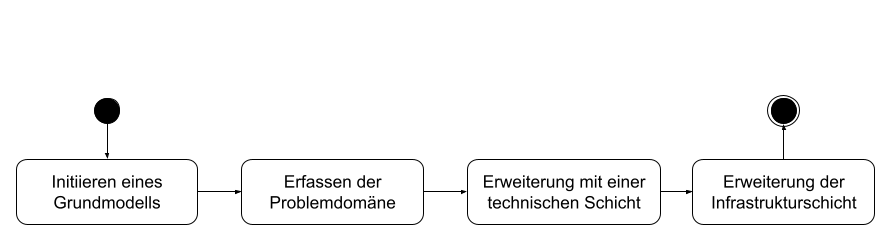
\includegraphics[width=\textwidth]{bilder/k5/workflow1.png}
\caption{Ein abstrakter Modellierungsworkflow für das Microservice-Metamodell}
\end{figure}


\newpage
\section{Entwurf des Editors}

Die verschiedenen Visualisierungen und Werkzeuge werden mit einer \glqq Sirius Viewpoint Specification\grqq{} umgesetzt. Grundlegend funktioniert dies analog zu den Methoden, die in der dieser Arbeit vorausgehenden Seminararbeit vorgestellt wurden \cite[S.11-13]{loeffler}.

Aufgrund der Komplexität des Metamodells ergeben sich grundlegende konzeptionelle Fragen, die vor der eigentlichen Umsetzung zu klären sind. Es hat sich gezeigt, dass der Versuch, allumfassende Modelldiagramme zu erstellen, kognitiv schwer nachvollziehbar war. Der ursprüngliche Ansatz, pro Schicht ein separates Diagramm zu verwenden, wurde daher verworfen. Stattdessen zielt die Neukonzeption der Diagramme darauf ab, einen effektiven Workflow zu unterstützen. Zudem soll der Einsatz verschachtelter Darstellungen, bei denen einzelne Grafiken als Elemente in übergeordneten Strukturen dienen, das Verständnis erleichtern und eine strukturierte Präsentation ermöglichen.

Zentral für den Entwurf sind verschiedene AQL-Ausdrücke, die genutzt werden, um Logik in der grafischen Oberfläche umzusetzen. So erweist sich die Umsetzung des Werkzeugs, das Microservices in der \glqq ContextRelationshipDescription\grqq{}, einem Diagramm welches die Beziehungen von BoundedContexts zueinander zeigt, erzeugt, als verhältnisweiße komplex:

\begin{lstlisting}[caption=Erzeugen eines Microservices als Border Node an einem Bounded Context]
//Precondition
aql:self.oclIsTypeOf(microserviceMetamodell::BoundedContext)

//Change Context to Right Container
aql:self.eContainer().eContainer().technicalLayer

//Setting the service name after creating the instance for the layer
aql:self.correspodingContext.contextName.toLower().concat('-service')

//Changing back to the container, the bounded context,
var:container
//and setting cotainer.correspondingMicroservices to the instance which was created before
var:instance
\end{lstlisting}

Dieser Ansatz musste öfters ähnlich angewandt werden. Grund hierfür ist die Entscheidung gegen Diagramme, welche nur die Schichtebene visualisieren. Dadurch muss an einigen Stellen auf hierarchisch höher liegende Container zugegriffen werden, um die passenden Objekte zu referenzieren. Weiterhin wird der Ansatz der typisierten Vorbedingung häufig genutzt.

Eine andere Art von Problematik ergibt sich bei der Darstellung durch rekursive Beziehungen von Elementen zu sich selbst. Dies soll am Beispiel der \glqq AggregateStructureDescription\grqq{}, welche die Struktur eines Aggregate visualisiert, verdeutlicht werden.

\newpage

\begin{figure}[ht]
\centering
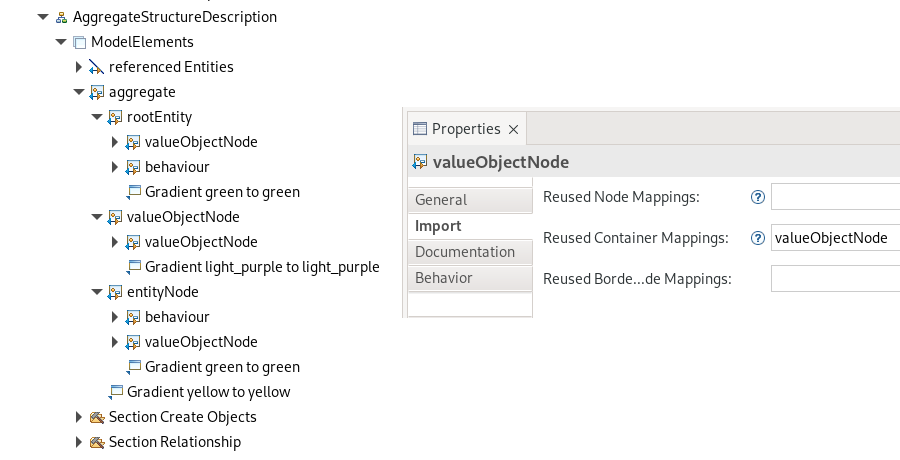
\includegraphics[width=0.7\textwidth]{bilder/k5/7.png}
\caption{Umsetzen von rekursiven Aufrufen durch das importieren von Nodes mit Sirius}
\end{figure}

Hier ist zu beachten, dass eine rekursive Beziehung, wie sie beispielsweise der ValueObjectNode aufweist, korrekt umgesetzt wird. Dazu muss der Node, der sich selbst enthält, sich selbst importieren, wie in der Abbildung zu sehen ist. Weiterhin stellt sich nun die Frage, ob eine Darstellung solcher rekursiven Beziehungen grundsätzlich sinnvoll ist.

\begin{figure}[ht]
\centering
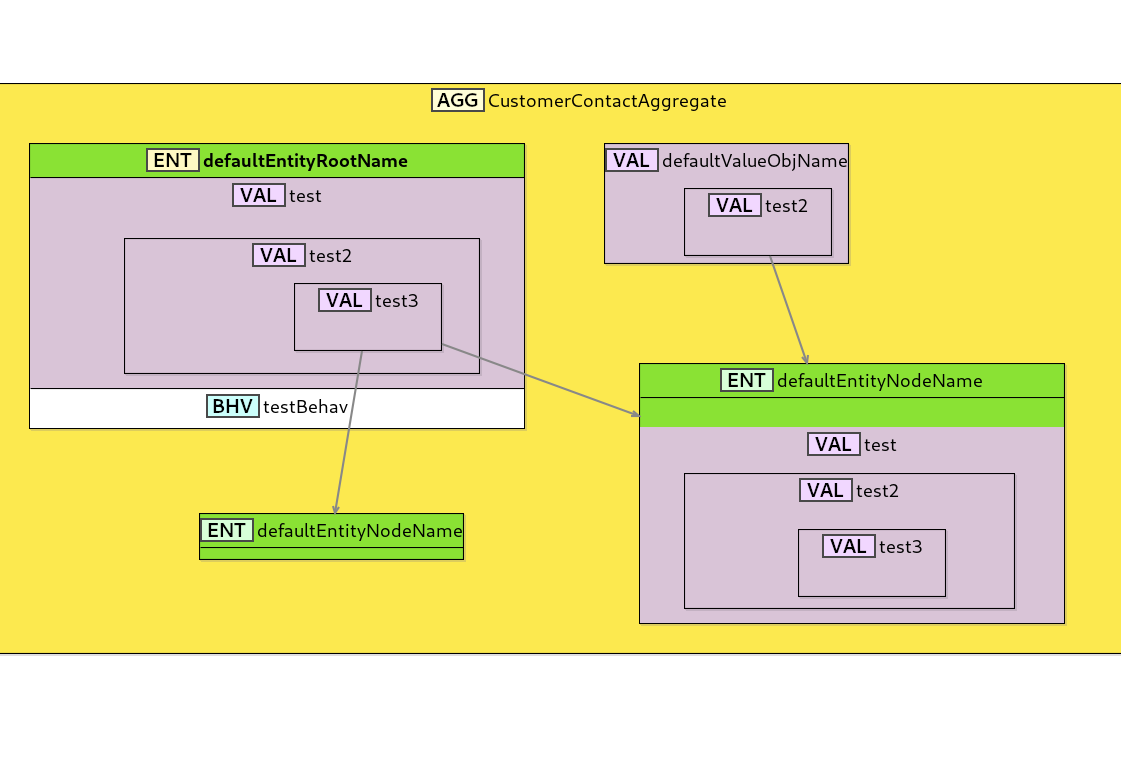
\includegraphics[width=0.8\textwidth]{bilder/k5/8.png}
\caption[Eine kognitiv anspruchsvolle Aggregate Visualisierung]{Eine kognitiv anspruchsvolle Aggregate Visualisierung - Hat ein Betrachter hier noch einen Mehrwert ?}
\end{figure}

Eine Modellierung von Klassenattributen in der Implementierung wurde bisher nicht berücksichtigt. Dies sollte im Rahmen der notwendigen Feinimplementierung händisch geschehen. Da außerdem auch andere EMF-Beschreibungsmodelle existieren, die für genau diese Aufgabe konzipiert wurden, wird die Entscheidung getroffen, keine Anpassung vorzunehmen und die Attributierung nicht konzeptionell in das Metamodell aufzunehmen. Fortschreitend werden für die Entity und das ValueObject keine feineren Strukturdiagramme entworfen. Konzeptionell würden diese jedoch symmetrisch zur AggregateStructureDescription umgesetzt werden.

%%%%%%%%%%%%%%%%%%%%%%%%%%%%%%%%%%%%%%%%%%%%%%%%%%%%%%%%%%%%%%%%%%%%%%%%%%%%%%%%%%%%%%%%%%%%%%%%%%%%%%%%%%%%%%%%%%%%
%			Diagramme
%%%%%%%%%%%%%%%%%%%%%%%%%%%%%%%%%%%%%%%%%%%%%%%%%%%%%%%%%%%%%%%%%%%%%%%%%%%%%%%%%%%%%%%%%%%%%%%%%%%%%%%%%%%%%%%%%%%%
\newpage
\section{Beschreibung der Diagramme}

\subsection{ContextRelationshipDescription}

Diese Darstellung zeigt die in einer DomainModelLayer vorhandenen BoundedContexts und ihre Beziehungen zueinander. Zweck des Diagramms ist die initiale Feststellung von Kontexten bei der Analyse einer Problemdomäne. Weiterhin können hier DomainModels und Microservices für einen Bounded Context erzeugt und implizit zugewiesen werden. Für eine Shared Kernel Beziehung, welche durch einen eigenen Container dargestellt wird, kann eine ExternalDependency ebenso erzeugt und implizit zugewiesen werden. Andere Beziehungstypen werden durch eine Auswahl im Eigenschaftsfenster mittels Radio-Buttons realisiert. Module können außerdem hier schon erzeugt werden, sofern einem BoundedContext ein DomainModel zugewiesen ist. Das Erzeugen eines Moduls in einem SharedKernel führt dabei zur Erstellung eines SharedModule.

\begin{figure}[ht]
\centering
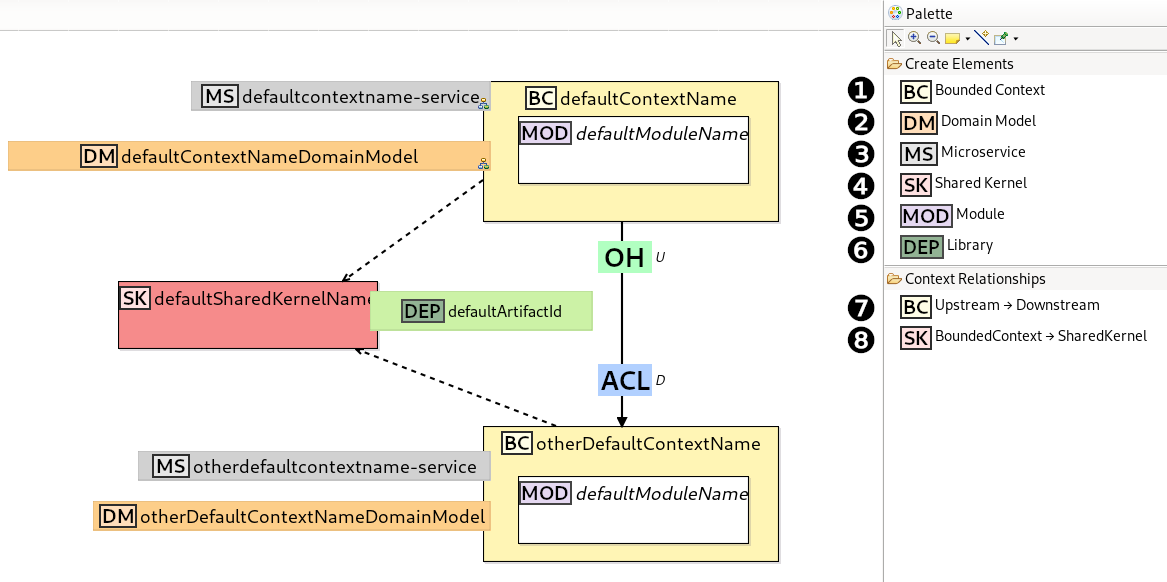
\includegraphics[width=\textwidth]{bilder/k5/1.png}
\caption{Editoransicht der ContextRelationshipDescription}
\end{figure}


\begin{table}[h]
\centering
\footnotesize
\begin{tabularx}{\textwidth}{|c|X|}
\hline
1 & Erzeugt ein BoundedContext. Namenskonvention: camelCase \\ \hline
2 & Erzeugt auf einem BoundedContext ein zugewiesenes DomainModel. Namenskonvention: camelCase \\ \hline
3 & Erzeugt auf einem BoundedContext ein zugewiesenen Microservice. Namenskonvention: kebap-case \\ \hline
4 & Erzeugt ein SharedKernel. Namenskonvention: camelCase \\ \hline
5 & Erzeugt auf einem BoundedContext oder SharedKernel ein (Shared)Module.\\ & Vorbedingung: Existierendes DomainModel. Namenskonvention: camelCase \\ \hline
6 & Erzeugt auf einem SharedKernel eine ExternalDependency.\\ & Namenskonvention: Abh. zu der Bezeichnung in mvnrepository \\ \hline
7 & Erzeugt Beziehung zwischen Quellkontext (Upstream) und Zielkontext (Downstream).\\ &  Nähere Typisierung im Eigenschaftsfenster \\ \hline
8 & Verbindet ein BoundedContext mit einem SharedKernel \\ \hline
\end{tabularx}
\caption{Legende - ContextRelationshipDescription}
\end{table}

\subsection{DomainModelDescription}

Die \glqq DomainModelDescription\grqq{} visualisiert ein DomainModel. Sie zeigt Module, die es enthält, sowie DomainEvents, die mit dem Modell assoziiert sind. Zudem stellt sie die verwendeten ModelElements dar und ermöglicht es dem Bearbeiter, diese nach Bedarf mit anderen Elementen des DomainModels zu verknüpfen. Außerdem visualisiert sie die in Entities und Aggregates enthaltenen Objekte.

\begin{figure}[ht]
\centering
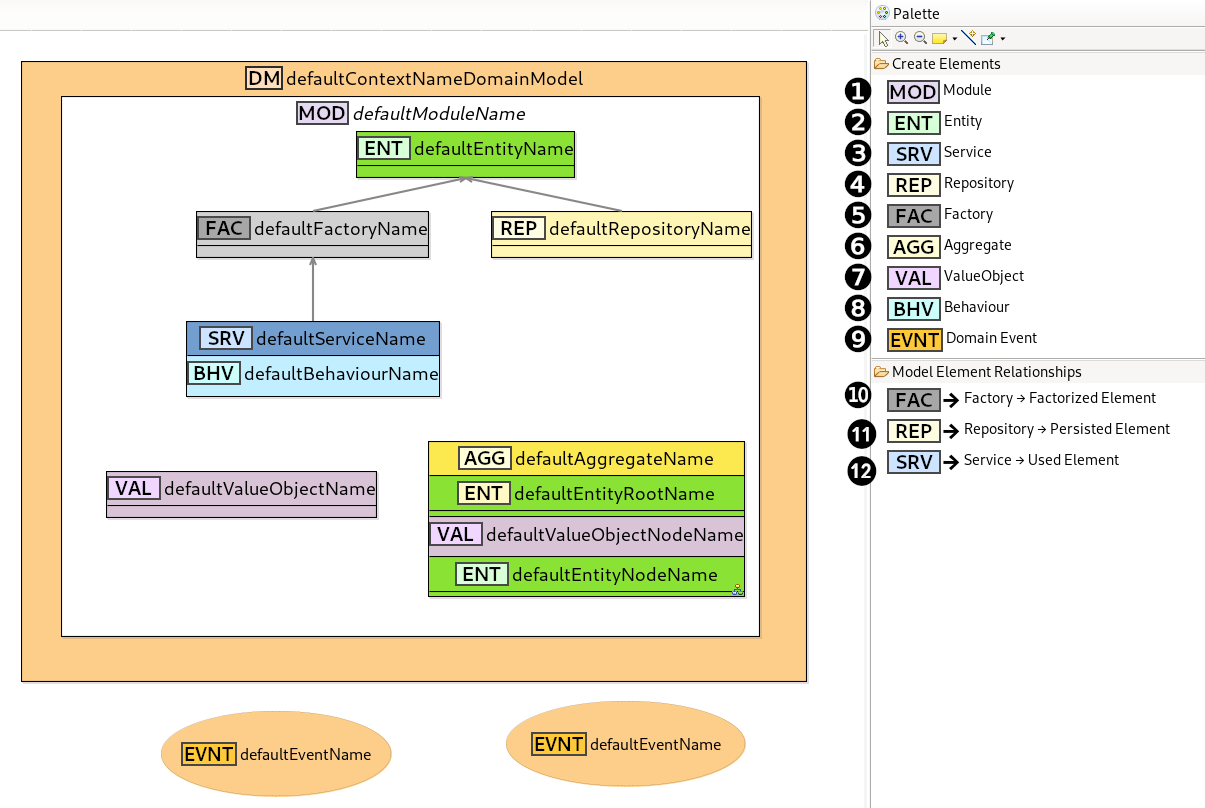
\includegraphics[width=\textwidth]{bilder/k5/2.png}
\caption{Editoransicht der DomainModelDescription}
\end{figure}


\begin{table}[h]
\centering
\footnotesize
\begin{tabularx}{\textwidth}{|c|X|}
\hline
1 & Erzeugt auf einem DomainModel ein enthaltenes Module. Namenskonvention: camelCase \\ \hline
2 & Erzeugt auf einem Module eine enthaltene Entity. Namenskonvention: camelCase \\ \hline
3 & Erzeugt auf einem Module einen enthaltenen Service. Namenskonvention: camelCase \\ \hline
4 & Erzeugt auf einem Module ein enthaltenes Repository. Namenskonvention: camelCase \\ \hline
5 & Erzeugt auf einem Module eine enthaltene Factory. Namenskonvention: camelCase \\ \hline
6 & Erzeugt auf einem Module ein enthaltenes Aggregate. Namenskonvention: camelCase \\ \hline
7 & Erzeugt auf einem Module ein enthaltenes ValueObject. Namenskonvention: camelCase \\ \hline
8 & Erzeugt auf geeigneten ModelElements ein Behaviour. Namenskonvention: camelCase \\ & Beim Repository zusätzlich: JPA konformer Funktionsname \\ \hline
9 & Erzeugt außerhalb des DomainModels ein zu diesem assoziiertes Event. Namenskonvention: keine \\ \hline
10 & Weist einer Factory ein Factorizable Element zu. \\ \hline
11 & Weist einem Repository ein Persistable Element zu. \\ \hline
12 & Weist einem Service ein Element zu. \\ \hline
\end{tabularx}
\caption{Legende - DomainModelDescription}
\end{table}

\newpage
\subsection{AggregateStructureDescription}

Um die kognitive Last, die durch komplexe Aggregates in der DomainModelDescription entstehen kann, zu reduzieren, wird eine AggregateStructureDescription genutzt. Diese spezialisiert sich auf die Darstellung der nach dem Metamodell verschachtelbaren Struktur. Diese wurde, wie bereits erläutert, zwar konzipiert, jedoch ist ihr Mehrwert diskutabel.

\begin{figure}[ht]
\centering
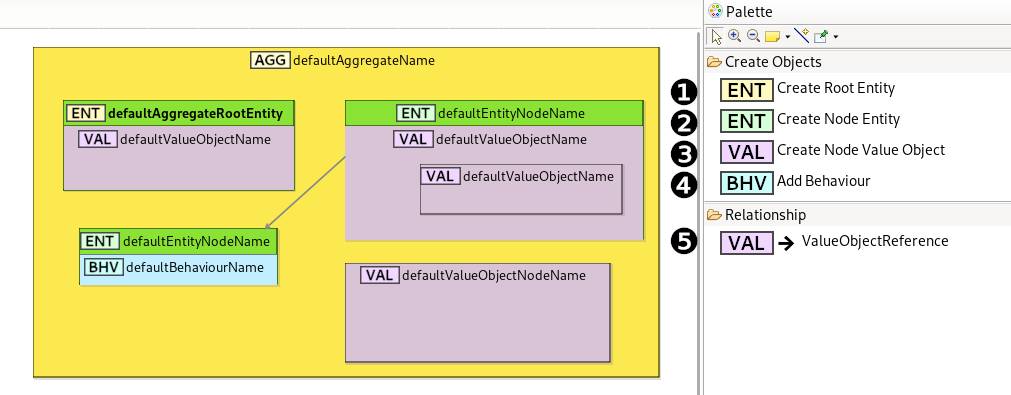
\includegraphics[width=\textwidth]{bilder/k5/3.png}
\caption{Editoransicht der AggregateStructureDescription}
\end{figure}


\begin{table}[h]
\centering
\footnotesize
\begin{tabularx}{\textwidth}{|c|X|}
\hline
1 & Erzeugt (eimalig) auf einem Aggregate eine dazugehörende EntityNode als Wurzel. Namenskonvention: camelCase \\ \hline
2 & Erzeugt auf einem Aggregate eine EntityNode als Blatt. Namenskonvention: camelCase \\ \hline
3 & Erzeugt auf einem Aggregate, einer Entity oder einem ValueObject ein enthaltenes ValueObject.\\ & Namenskonvention: camelCase \\ \hline
4 & Erzeugt auf einer Entity ein Behaviour. Namenskonvention: camelCase \\ \hline
5 & Weist einem ValueObject eine referenzierte Entity zu \\ \hline
\end{tabularx}
\caption{Legende - AggregateStructureDescription}
\end{table}

\newpage
\subsection{MicroserviceCommunicationDescription}

Die \glqq MicroserviceCommunicationDescription\grqq{} zeigt die Microservices in der technischen Schicht. Interfaces können hier betrachtet und verwaltet werden. Durch die zusätzliche Visualisierung der DomainEvents, die dem Microservice zugehörigen DomainModel zugewiesen sind, kann der Betrachter sich bei der Modellierung an diesen orientieren, um AsynchronousInterface Objekte zu verorten. SynchronousInterfaces können hier RestEndpoints zugewiesen werden. AsynchronousInterfaces können weiterhin Topics zugewiesen werden. Mit Werkzeugen zum Verbinden der Kommunikationsteilnehmer kann hier somit eine vollständige Übersicht der Kommunikationsabläufe in einer Microservice-Architektur umgesetzt werden.

\begin{figure}[ht]
\centering
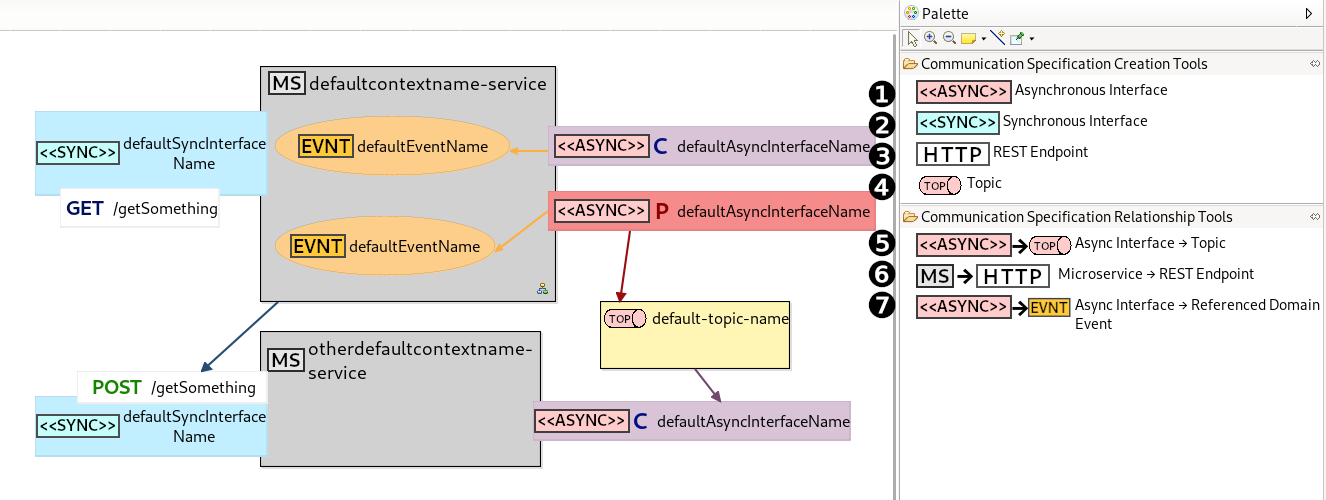
\includegraphics[width=\textwidth]{bilder/k5/4.png}
\caption{Editoransicht der MicroserviceCommunicationDescription}
\end{figure}


\begin{table}[h]
\centering
\footnotesize
\begin{tabularx}{\textwidth}{|c|X|}
\hline
1 & Erzeugt auf einem Microservice ein zugewiesenes AsynchronousInterface. Namenskonvention: camelCase   \\ \hline
2 & Erzeugt auf einem Microservice ein zugewiesenes SynchronousInterface. Namenskonvention: camelCase \\ \hline
3 & Erzeugt auf einem SynchronousInterface einen zugewiesenen RestEndpoint. Namenskonvention: "/" + camelCase \\ \hline
4 & Erzeugt ein neues Topic. Setzt existierende KafkaConfiguration voraus. Namenskonvention: kebap-case\\ \hline
5 & Weist einem AsynchronousInterface ein Topic zu.\\ & Datenflussrichtung wird implizit aus Rolle der Schnittstelle bestimmt. \\ \hline
6 & Weist einem Microservice einen zu aufrufenden RestEndpoint zu. \\ \hline
7 & Weist einem AsynchronousInterface ein Event zu. \\ \hline
\end{tabularx}
\caption{Legende - MicroserviceCommunicationDescription}
\end{table}

\newpage
\subsection{MicroserviceInterfaceDescription}

Die folgende \glqq MicroserviceInterfaceDescription\grqq{} dient der Darstellung und Verwaltung der Kommunikation und deren Ursprung auf Service-Ebene. Daher werden Relationen aus dem DomainModel ausgeblendet. Zusätzlich werden Interfaces des Dienstes und RestEndpoints anderer Dienste, die dem Microservice zugewiesen sind, visualisiert. Das Anlegen und Zuweisen dieser externen Schnittstellen wird nur in der MicroserviceCommunicationDescription umgesetzt, um die kognitive Last dieser Beschreibung zu reduzieren.

\begin{figure}[ht]
\centering
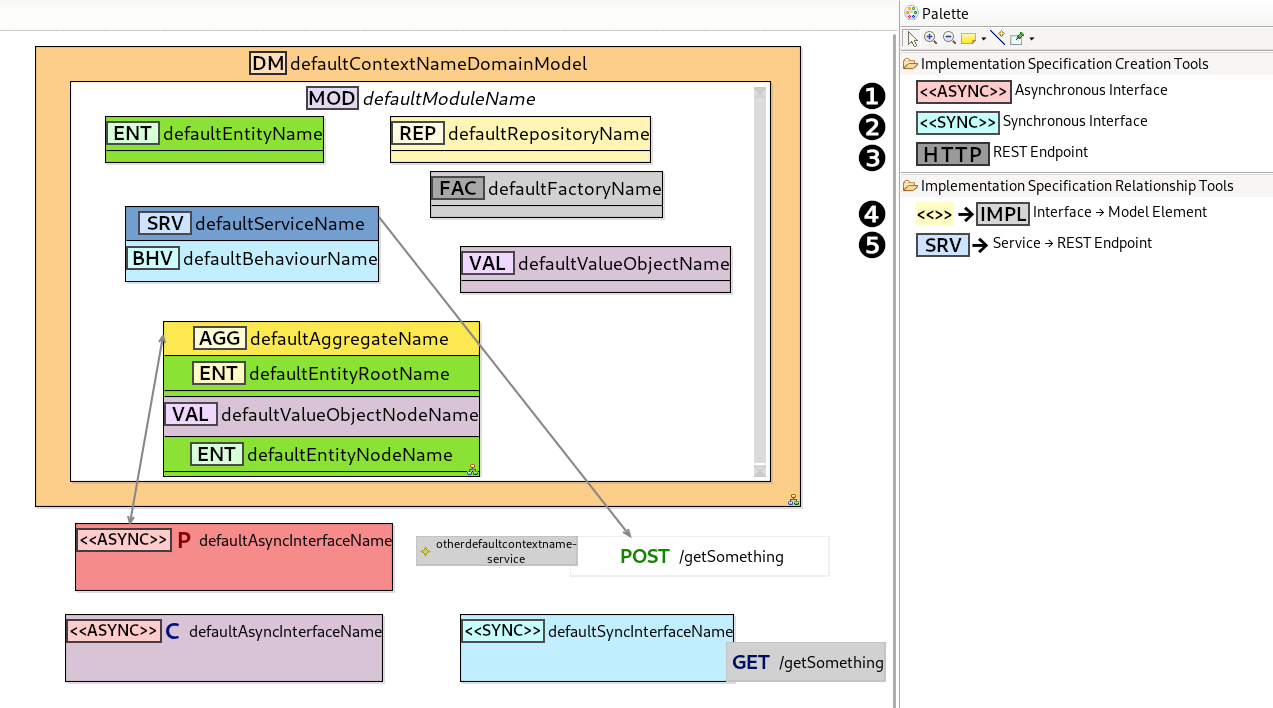
\includegraphics[width=\textwidth]{bilder/k5/5.png}
\caption{Editoransicht der MicroserviceInterfaceDescription}
\end{figure}

\begin{table}[h]
\centering
\footnotesize
\begin{tabularx}{\textwidth}{|c|X|}
\hline
1 & Erzeugt ein AsynchronousInterface. Namenskonvention: camelCase\\ \hline
2 & Erzeugt ein SynchronousInterface. Namenskonvention: camelCase \\ \hline
3 & Erzeugt auf einem SynchronousInterface einen RestEndpoint.\\ & Namenskonvention: "/" + camelCase\\ \hline
4 & Weist einem Interface referenzierte ModelElements zu. \\ \hline
5 & Weist einem Service einen externen, zu aufrufenden RestEndpoint zu. \\ \hline
\end{tabularx}
\caption{Legende - MicroserviceInterfaceDescription}
\end{table}

\newpage
\subsection{InfrastructureOverviewDescription}

Schließlich wird in der \glqq InfrastructureOverviewDescription\grqq{} die Infrastrukturschicht dargestellt. Hier werden vor allem Konfigurationen angelegt und diese den existierenden Microservices zugewiesen. Weiterhin werden zusätzliche modellierte Abhängigkeiten dargestellt.

\begin{figure}[ht]
\centering
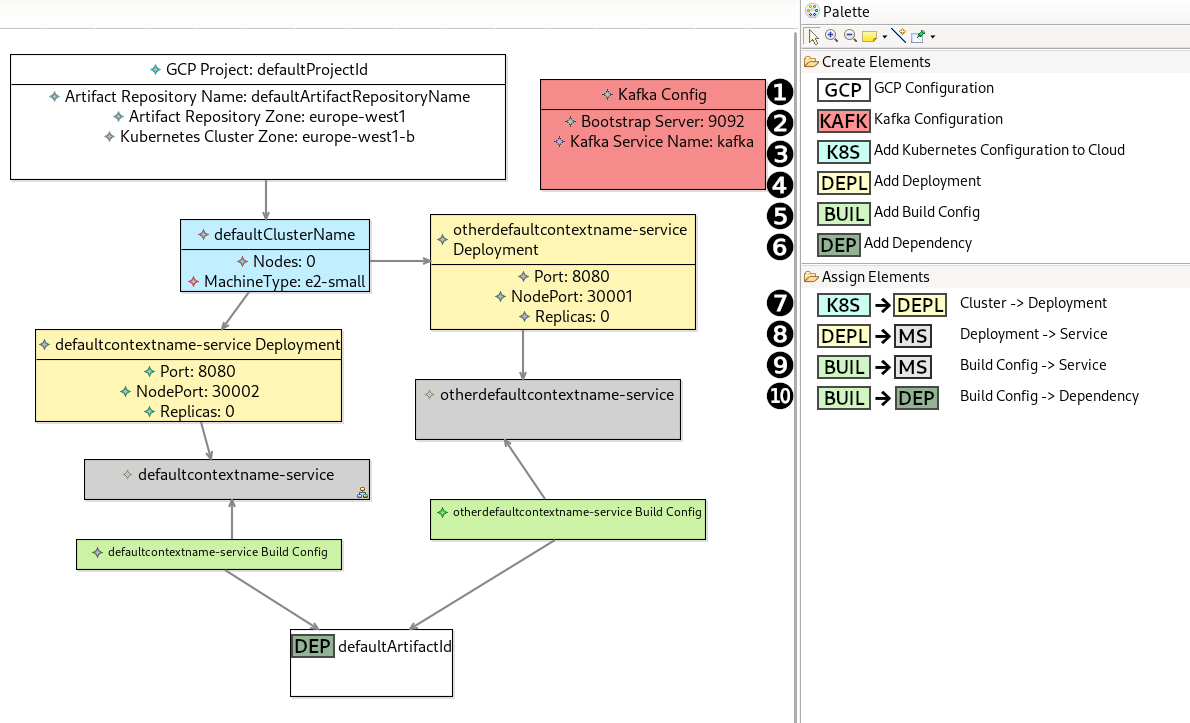
\includegraphics[width=\textwidth]{bilder/k5/6.png}
\caption{Editoransicht der InfrastructureOverviewDescription}
\end{figure}

\begin{table}[h]
\centering
\footnotesize
\begin{tabularx}{\textwidth}{|c|X|}
\hline
1 & Erzeugt eine GCloudConfiguration. Namenskonvention: Der GCP zu entnehmen, kebap-case \\ \hline
2 & Erzeugt eine KafkaConfiguration. Namenskonvention: kebap-case \\ \hline
3 & Erzeugt eine KubernetesClusterConfiguration. Namenskonvention: kebap-case \\ \hline
4 & Erzeugt eine DeploymentConfiguration. Namenskonvention: Generiert \\ \hline
5 & Erzeugt eine BuildConfiguration. Namenskonvention: Generiert \\ \hline
6 & Erzeugt eine ExternalDependency. Namenskonvention: Äquivalent zur Bennenung in mvnrepository \\ \hline
7 & Weist einer KubernetesClusterConfiguration DeploymentConfigurations zu. \\ \hline
8 & Weist einer DeploymentConfiguration einen Service zu. \\ \hline
9 & Weist einer BuildConfiguration einen Service zu. \\ \hline
10 & Weist einer BuildConfiguration eine Dependency zu. \\ \hline
\end{tabularx}
\caption{Legende - InfrastructureOverviewDescription}
\end{table}

\newpage

\section{Konkretisierung des Modellierungsworkflows}

Auf Basis des abstrakten Modellierungsworkflows wird nun ein konkreter Workflow, der den konzipierten Editor und die dazugehörige konkrete Syntax verwendet, definiert. Dazu kann beginnend eine dem Quellcodeverzeichnis beiliegende Modellvorlage \cite{mustermodell} verwendet werden. Alternativ können die notwendigen Klassen, die in Abbildung 5.10 aufgezählt werden, händisch in ein leeres EMF-Modell eingefügt werden. Der Schritt des Erfassens der Problemdomäne erfolgt durch das sequenzielle Anlegen der ContextRelationshipDescription, der DomainModelDescriptions (je DomainModel) und der AggregateStructureDescriptions. Darauf folgt die Konzeption der technischen Schicht mittels MicroserviceCommunicationDescription und MicroserviceInterfaceDescription (je Microservice). Abschließend wird mit der InfrastructureOverviewDescription die nötige Infrastruktur modelliert.

\begin{figure}[ht]
\centering
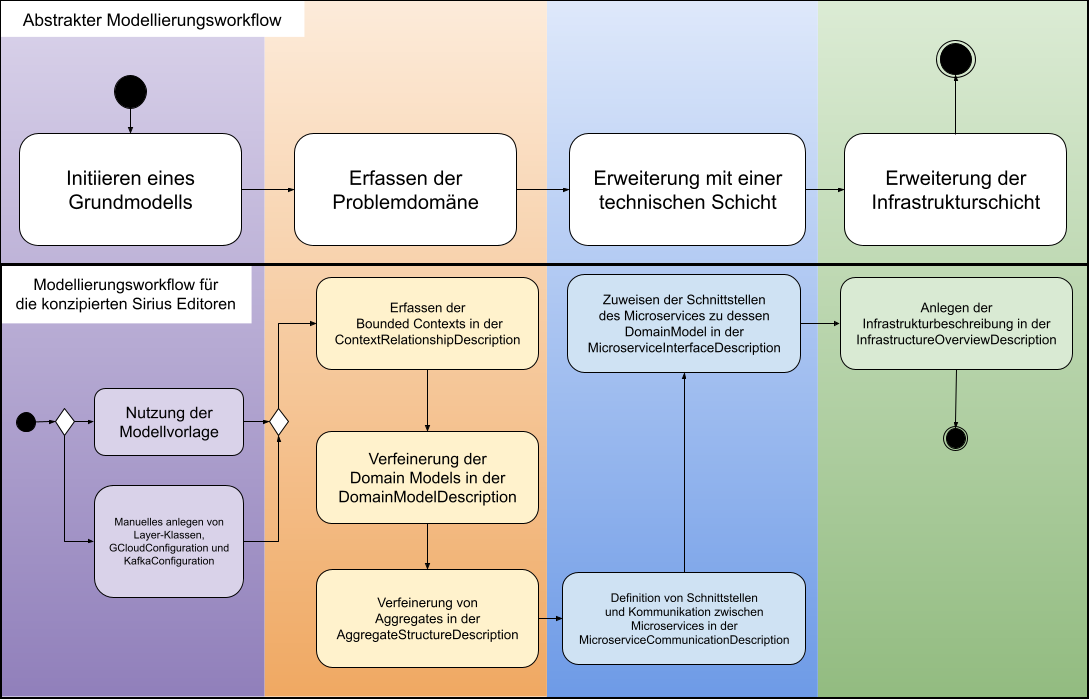
\includegraphics[width=\textwidth]{bilder/k5/workflow2.png}
\caption{Abbildung des abstrakten Modellierungsworkflows auf einem für diesen Editor angepassten Workflow}
\end{figure}

\chapter{Konzeption und Umsetzung der Codegenerierung}

Basierend auf dem Metamodell soll eine Codegenerierung mit dem Acceleo-Codegenerator konzipiert werden. Dabei soll durch ein Generierungstemplate Code erzeugt werden, der Java/Spring-Applikationen umsetzt, welche mit Docker als Images ausgeführt werden können. Nutzer sollen weiterhin einfach Deployments in eine existierende Google-Cloud-Umgebung ausführen können. Abgegrenzt von der Generierung wird die konkrete Implementierung von Funktionen, die Datenstruktur von Entities und ValueObjects sowie detailliertere Inhalte der Kommunikation (wie z.B.: HTTP-Headers, Request Bodies oder Kafka-Nachrichtenstruktur).

Dafür werden folgende Anforderungen an die lokale Ausführungsumgebung gestellt:
\begin{itemize}
  \item Ein Linux-Betriebssystem mit einer Bash-Shell
  \item Installierte Google Cloud CLI \cite{gcloudsdk}
  \item Installiertes Kubernetes Befehlszeilenprogramm kubectl \cite{kubernetes}
  \item Authentifizierung von kubectl durch das gke-gcloud-auth-plugin \cite{kubernetesauth}
  \item Installiertes Docker Desktop \cite{docker}
  \item Installiertes Gradle \cite{gradle}
\end{itemize}

\section{Generierungstemplate}

Das Generierungstemplate erzeugt zunächst Dateien, die nur einmal für die gesamte Architektur existieren müssen. Diese werden genutzt, um die generierten Microservices zu bauen und Deployments auszuführen. Sie befinden sich in einem Verzeichnis namens \glqq bash_scripts\grqq{}. Anschließend durchläuft das Template drei Hauptiterationen: Eine über alle Microservices, eine über alle Module und Modellelemente und abschließend eine über alle Schnittstellen. Hierbei wird je Service ein eigenes Verzeichnis angelegt, in dem sich nach der Generierung die servicespezifischen Dateien in einer typischen Projektstruktur wiederfinden. Im Folgenden wird die Struktur des Generierungstemplates tabellarisch vorgestellt und kurz auf die erzeugten Klassen eingegangen.

\newpage

\begin{table}[h]
\centering
\footnotesize
\begin{tabularx}{\textwidth}{ | l | c | c | c | X | }
\hline
\textbf{Dateiname} & \textbf{S} & \textbf{M} & \textbf{I} & \textbf{Beschreibung} \\ 
\hline
setup_kubernetes_cluster.sh &  &  &  & Erzeugt ein neues Kubernetes Cluster \\ 
\hline
setup_docker_registry.sh &  &  &  & Erzeugt eine neue Artifact Repository \\ 
\hline
check_gcp_and_cluster.sh &  &  &  & Überprüft Verfügbarkeit von GCP und Kubernetes Cluster \\ 
\hline
setup_kafka.sh &  &  &  & Startet Kafka Container und Kubernetes Service \\
\hline
delete_kafka.sh &  &  &  & Entfernt Kafka Container und Service im Cluster \\ 
\hline
create_topics.sh &  &  &  & Erzeugt bei laufendem Kafka Container neue Topics \\ 
\hline
deployment.yml &  &  &  & Kubernetes Deployment für Kafka \\ 
\hline
whitelist_ip.sh &  &  &  & Setzt IP des Users als einzig erlaubte IP für das Cluster \\ 
\hline
deploy_services.sh &  &  &  & Führt Deployment aus und konfiguriert Firewall \\ 
\hline
undeploy_services.sh &  &  &  & Macht Deployment und Firewall rückgängig \\ 
\hline
add_wrapper.sh &  &  &  & Fügt Gradle Wrapper zu jedem Service hinzu \\ 
\hline
build_images.sh &  &  &  & Baut Images für Services und pusht diese \\ 
\hline
healthcheck.sh &  &  &  & Schickt einen GET Request gegen alle Health Endpunkte \\
\hline
get_cluster_info.sh &  &  &  & Gibt Informationen zum Cluster aus \\ 
\hline
scale_down_cluster.sh &  &  &  & Setzt die Cluster Nodes auf 0 und damit das Cluster inaktiv \\ 
\hline
scale_up_cluster.sh &  &  &  & Setzt die Cluster Nodes auf 1 \\ 
\hline
cleanup_registry.sh &  &  &  & Entfernt alle Images im Artifact Repository \\ 
\hline
delete_cluster.sh &  &  &  & Löscht das Kubernetes Cluster \\ 
\hline
delete_registry.sh &  &  &  & Löscht die Artifact Registry \\ 
\hline
execute_local.sh &  &  &  & Führt Services lokal aus \\ 
\hline
cancel_execute_local.sh &  &  &  & Beendet lokal gestartete Microservices \\ 
\hline
kafka_local.sh &  &  &  & Führt Kafka lokal aus \\
\hline
ApplicationStarter.java & • &  &  & Einstiegspunkt für die Spring Boot Anwendung \\ 
\hline
application.yml & • &  &  & Anwendungseigenschaften \\
\hline
build.gradle & • &  &  & Build Konfiguration und Abhängigkeitsverwaltung \\
\hline
deployment.yml & • &  &  & Servicesspezifisches Kubernetes Deployment \\
\hline
build_and_push.sh & • &  &  & Baut Anwendungsimage und pusht dieses in die Cloud \\
\hline
Dockerfile & • &  &  & Beschreibt Docker Image \\
\hline
HealthCheckController.java & • &  &  & Schnittstelle für Healthcheck \\
\hline
WebSecurityConfiguration.java & • &  &  & Setzt Schnitstellensicherheit. Definiert Endpunkte public. \\
\hline
WebClientConfig.java & • &  &  & Benötigt für die Bean Injection des WebClient. \\
\hline
EntityName.java & • & • &  & Erzeugt JPA konforme Entity mit ID \\
\hline
ValueObjectName.java & • & • &  & Erzeugt Klassenrumpf \\
\hline
AggregateName.java & • & • &  & Erzeugt JPA konformes Aggregate mit ID und Nodes \\
\hline
EntityNodeName.java & • & • &  & Erzeugt JPA konforme Entity mit ID  \\
\hline
ValueObjectNodeName.java & • & • &  & Erzeugt Klassenrumpf \\
\hline
ServiceName.java & • & • &  & Erzeugt Service Komponente \\
\hline
FactoryName.java & • & • &  & Erzeugt Factory Komponente für zugewiesene Klasse \\
\hline
RepositoryName.java & • & • &  & Erzeugt JPA Repository für zugewiesene Klasse \\
\hline
SyncInterfaceName.java & • &  & • & Erzeugt einen Spring Controller mit Endpunkten \\
\hline
AsyncInterfaceConsumerName.java & • & & • & Erzeugt eine Kafka Consumer als Komponente \\
\hline
AsyncInterfaceProducerName.java & • & & • & Erzeugt eine Kafka Producer als Komponente \\
\hline
\end{tabularx}
\caption{Übersicht der generierten Dateien}
\end{table}

\textbf{Legende:}
\begin{itemize}
    \item[\textbf{S}] - Iteration über alle Microservices
    \item[\textbf{M}] - Iteration über alle Module und Modellelemente
    \item[\textbf{I}] - Iteration über alle Schnittstellen
\end{itemize}

\newpage

Detailierter soll nun auf eine konkrete Implementierung einer Metamodellklasse eingegangen werden. Dafür wird die Klasse Service näher betrachtet. Diese erwies sich in ihrer Umsetzung als am komplexesten. Im Folgenden wird auf die verwendeten Lösungen näher eingegangen und die Funktionsweise der resultierenden Java Datei angeschnitten.

\begin{lstlisting}[caption=Importieren anderer Klassen]
[if modelElement.oclIsTypeOf(microserviceMetamodell::Service)]
[file ('/' + microservice.serviceName + '/src/main/java/app/' + module.moduleName + '/' + modelElement.elementName + '.java', false, 'UTF-8')] 
package app.[module.moduleName/];

import org.slf4j.Logger;
import org.slf4j.LoggerFactory;
import org.springframework.stereotype.Service;

[for( element: ModelElement | modelElement.oclAsType(microserviceMetamodell::Service).referencedElements)]
import app.[element.eContainer().oclAsType(microserviceMetamodell::Module).moduleName/].[element.elementName/];
[/for]

[if modelElement.oclAsType(microserviceMetamodell::Service).sendsRequestTo->notEmpty()]
import org.springframework.web.reactive.function.client.WebClient;
import reactor.core.publisher.Mono;
import org.springframework.beans.factory.annotation.Value;
[/if]

[for( interface: Interface | modelElement.oclAsType(microserviceMetamodell::Service).referencedInterfaces)]
	[if interface.oclIsKindOf(microserviceMetamodell::AsynchronousInterface)]
			[if interface.oclAsType(microserviceMetamodell::AsynchronousInterface).interfaceRole = (microserviceMetamodell::AsynchronousInterfaceRole::PRODUCER)]
import app.kafka.[interface.interfaceName/];
			[/if]
	[/if]
[/for]
\end{lstlisting}

Der in Quellcode 6.1 dargestellte Code überprüft die Iteration aller Modellelemente auf die Klasse Service und erzeugt diese gegebenenfalls mit der passenden Paketdefinition. Mithilfe von Java-Importausdrücken werden dann die benötigten Klassen eingebunden. Dies wird durch eine Iteration über alle referenzierten Objekte umgesetzt. Weiterhin gibt es Imports, die nicht unbedingt vorhanden sein müssen. Die erforderlichen WebClient-Imports werden beispielsweise nur dann erzeugt, wenn entsprechende Zielschnittstellen existieren. Auch für asynchrone Schnittstellen erfolgt eine bedingte Erzeugung, die davon abhängig ist, ob sie in der erzeugten Klasse verwendet wird. Zusätzlich wird mit einer bedingten Abfrage eingefordert, dass die Schnittstelle vom Typ Producer ist.
\newpage
Dies liegt daran, dass trotz der allgemeinen Assoziation \glqq referencedInterfaces\grqq{} ein Service nur von Producern sinnvoll verwendet werden kann. Dies resultiert aus der Verwendung dieser als sendende Schnittstelle. Empfangende Schnittstellen hingegen werden beim Empfang erst selbst aktiv und müssten dementsprechend den Service referenzieren.

\begin{lstlisting}[caption=Klassenattribute]
@Service
public class [modelElement.elementName/] {

    Logger logger = LoggerFactory.getLogger([modelElement.elementName/].class);

[for( element: ModelElement | modelElement.oclAsType(microserviceMetamodell::Service).referencedElements)]
	[if not element.oclIsKindOf(microserviceMetamodell::Factorizeable)]
	private final [element.elementName/] [element.elementName.toLowerFirst()/];
	[/if]
[/for]

[for( interface: Interface | modelElement.oclAsType(microserviceMetamodell::Service).referencedInterfaces)]
	[if interface.oclIsKindOf(microserviceMetamodell::AsynchronousInterface)]
		[if interface.oclAsType(microserviceMetamodell::AsynchronousInterface).interfaceRole = (microserviceMetamodell::AsynchronousInterfaceRole::PRODUCER)]
	private final [interface.interfaceName/] [interface.interfaceName.toLowerFirst()/];
		[/if]
	[/if]
[/for]

[comment]Using the Correct Urls - As communication targets must be distinct, a more compley approach is needed here[/comment]
[if (modelElement.oclAsType(microserviceMetamodell::Service).sendsRequestTo->notEmpty())]
    private final WebClient webClient;

    [let allServiceNames : Set(String) = modelElement.oclAsType(microserviceMetamodell::Service).sendsRequestTo->collect(restEndpoint | restEndpoint.ancestors(microserviceMetamodell::Microservice)->first().serviceName.toString())->asSet()]
        [for (service : String | allServiceNames)]
            @Value("${external-services.[service/].base-url}")
            private String [service.replace('-service', '')/]BaseUrl;
        [/for]
    [/let]

[/if]
\end{lstlisting}

\newpage

Quellcode 6.2 zeigt die korrekte Erzeugung der Klassenattribute. Aufgrund des Dependency-Injection-Konzepts von Spring-Anwendungen gibt es keine Klassenattribute für Klassen, die das Factorizeable-Interface implementieren. Diese würden bedarfsgesteuert erzeugt werden. Wie bei den Importen werden auch hier Producer nur generiert, wenn sie verwendet werden. Falls ein Service andere Schnittstellen über REST aufrufen möchte, muss ein Attribut für den WebClient gesetzt werden. Ein WebClient sendet Anfragen an die URLs, die in den Anwendungsvariablen, also der application.yml, referenziert sind. Um dies korrekt umzusetzen, ist es notwendig, eine disjunkte Menge zu erzeugen, in der alle Ursprungsservices der referenzierten Endpunkte enthalten sind. Dies wird durch die Filterung der Vorfahrenliste, der Umwandlung in ein einzelnes Element und der Konvertierung in den Typen Set erreicht. Anschließend kann über die resultierende disjunkte Menge aller Servicenamen iteriert werden.

\begin{lstlisting}[caption=Konstruktorparameter]
[comment]The Constructor Parameters for a Service Class - The correct placement of the comma in all cases makes this complex[/comment]
	[modelElement.elementName/](
[for( element: ModelElement | modelElement.oclAsType(microserviceMetamodell::Service).referencedElements)]
	[if not element.oclIsKindOf(microserviceMetamodell::Factorizeable)]
	[element.elementName/] [element.elementName.toLowerFirst()/]
		[if not modelElement.oclAsType(microserviceMetamodell::Service).referencedElements->last().elementName.equalsIgnoreCase(element.elementName)]
	,
		[/if]
	[/if]
[/for]

[for( interface: Interface | modelElement.oclAsType(microserviceMetamodell::Service).referencedInterfaces)]
	[if interface.oclIsKindOf(microserviceMetamodell::AsynchronousInterface)]
		[if interface.oclAsType(microserviceMetamodell::AsynchronousInterface).interfaceRole = (microserviceMetamodell::AsynchronousInterfaceRole::PRODUCER)]
			[if modelElement.oclAsType(microserviceMetamodell::Service).referencedElements->notEmpty()]
				[if not modelElement.oclAsType(microserviceMetamodell::Service).referencedElements->exists(e | e.oclIsKindOf(microserviceMetamodell::Factorizeable))]
					[if modelElement.oclAsType(microserviceMetamodell::Service).referencedInterfaces->first().interfaceName.equalsIgnoreCase(interface.interfaceName)]
		,
					[/if]
				[/if]
			[/if]
		[interface.interfaceName/] [interface.interfaceName.toLowerFirst()/]
			[if not modelElement.oclAsType(microserviceMetamodell::Service).referencedInterfaces->last().interfaceName.equalsIgnoreCase(interface.interfaceName)]
		,
			[/if]
		[/if]
	[/if]
[/for]

[if modelElement.oclAsType(microserviceMetamodell::Service).sendsRequestTo->notEmpty()]
	[if modelElement.oclAsType(microserviceMetamodell::Service).referencedElements->notEmpty()]
		[if modelElement.oclAsType(microserviceMetamodell::Service).referencedInterfaces->select(interface | interface.oclIsKindOf(microserviceMetamodell::AsynchronousInterface))->notEmpty()]
		,
		[/if]
	[/if]
		WebClient webClient
[/if]
)
\end{lstlisting}

Der Code aus den Quellen 8.3 und 8.4 zeigt die korrekte Erzeugung des Klassenkonstruktors. Dabei werden die notwendigen Klassenattribute als Konstruktorparameter übergeben und im Konstruktorrumpf gesetzt. Insbesondere die korrekte Setzung der Kommas erweist sich als äußerst kompliziert. Hierbei muss zunächst bedacht werden, dass ein Komma explizit nicht gesetzt wird, wenn das letzte Element der \glqq referencedElements\grqq{} im Konstruktor aufgelistet wurde. Die darauf folgenden Schnittstellen-Konstruktorparameter müssen neben der bereits geschilderten Differenzierung zwischen Producern und Consumern ebenfalls eine besondere Kommasetzung berücksichtigen. Hier darf kein Komma gesetzt werden, wenn der Service ModelElements referenziert oder nur solche referenziert werden, die nicht als Attribute existieren und somit das Factorizeable-Interface implementieren. Außerdem muss für den Fall, dass mehrere Producer existieren, eine gesonderte Kommasetzung beachtet werden.

\newpage

\begin{lstlisting}[caption=Konstruktorrumpf]
[comment]Constructor Values[/comment]
{
[for( element: ModelElement | modelElement.oclAsType(microserviceMetamodell::Service).referencedElements)]
		this.[element.elementName.toLowerFirst()/] = [element.elementName.toLowerFirst()/];
[/for]

[for( interface: Interface | modelElement.oclAsType(microserviceMetamodell::Service).referencedInterfaces)]
	[if interface.oclIsKindOf(microserviceMetamodell::AsynchronousInterface)]
		[if interface.oclAsType(microserviceMetamodell::AsynchronousInterface).interfaceRole = (microserviceMetamodell::AsynchronousInterfaceRole::PRODUCER)]
		this.[interface.interfaceName.toLowerFirst()/] = [interface.interfaceName.toLowerFirst()/];
		[/if]
	[/if]
[/for]

[if modelElement.oclAsType(microserviceMetamodell::Service).sendsRequestTo->notEmpty()]
    	this.webClient = webClient;
[/if]
}
\end{lstlisting}

Der Konstruktorrumpf muss nur die bisher schon beschriebenen Sonderfälle berücksichtigen. Das korrekte Setzen des Semikolons zeigt sich für die Sprache Java in Relation zu den Kommas der Konstruktorparameter als einfacher.

\begin{lstlisting}[caption=Methoden]
[comment]Behaviours[/comment]
[for ( behaviour: Behaviour | modelElement.oclAsType(microserviceMetamodell::Service).behaviours)]
	public void [behaviour.behaviourName/](){
		logger.info("[behaviour.behaviourName/] executed");
		//TODO: Implement Behaviour
	}
[/for]
\end{lstlisting}

\newpage

Für die modellierten Objekte der Klasse Behaviour werden Methodenköpfe generiert. Diese werden standardmäßig mit einem Logging, einem \glqq TODO\grqq{} und dem Rückgabetypen \glqq void\grqq{} generiert.

\begin{lstlisting}[caption=WebClient Implementierung]
[comment]Calls to other Microservices[/comment]
[for (restEndpoint : RestEndpoint | modelElement.oclAsType(microserviceMetamodell::Service).sendsRequestTo)]
    [let serviceName : String = restEndpoint.ancestors(microserviceMetamodell::Microservice)->first().serviceName.toString()]
        private Mono<String> request[restEndpoint.path.toString().substring(2).toUpperFirst()/]() {
            logger.info("request[restEndpoint.path.toString().substring(2).toUpperFirst()/] executed");
            return webClient.[restEndpoint.httpMethod.toString().toLowerCase()/]()
                    .uri([serviceName.replace('-service', '')/]BaseUrl + "[restEndpoint.path/]")
					.retrieve()
					.bodyToMono(String.class);
		}
	[/let]
[/for]
}
[/file]
[/if]
\end{lstlisting}

Die Generierung des WebClient-Aufrufs erstellt eine passende Implementierung basierend auf dem Zielservice und dem HTTP-Typ. Es ist zu beachten, dass einmalig der Zielpfad angepasst wird, um den führenden Schrägstrich zu entfernen. Konkretere Aufrufseigenschaften wie Header oder Body wurden nicht in der Generierung berücksichtigt. Abschließend wird mit dem schließenden File-Tag das Ende der generierten Klasse markiert.

Andere zu generierende Klassen wurden ähnlich, jedoch mit geringerer Komplexität umgesetzt. Wiederkehrende AQL-Funktionalitäten umfassen das Prüfen und Casten von Klassen, die Iteration, bedingte Ausdrücke und die Weiterverarbeitung von Ergebnissen, wie Listen, mithilfe von Funktionen wie \glqq{}notEmpty()\grqq{} oder \glqq first()\grqq{}.

\newpage

\section{Migration von Diensten durch Generierung}

Aufgrund von veränderten Anforderungen oder Aktualisierungen von Bibliotheken, kann es notwendig sein, dass der generierte Quellcode migriert werden muss. Dieses im Software-Lebenszyklus wiederkehrende Problem wirft die Frage auf, wie der bisherige modellgetriebene Entwicklungsansatz damit umgehen könnte. Dabei muss bedacht werden, was mit Code geschieht, der auf Basis der bisher konzipierten Codegenerierung ergänzend hinzugefügt wurde.

\subsection{Acceleo Protected Areas}

Ein Ansatz wären geschützte Bereiche, die mit der AQL definiert werden können. Dies lässt sich im folgenden Quellcode betrachten. Mittels des Schlüsselwortes \glqq protected\grqq{} werden diese beispielsweiße innerhalb von Methoden definiert. Die dadurch markierten Codeblöcke werden nach der initialen Generierung nicht mehr neu erzeugt.

\begin{lstlisting}[caption=Einsatz von geschützen Bereichen im Generierungstemplate]
[comment]Behaviours[/comment]
[for ( behaviour: Behaviour | modelElement.oclAsType(microserviceMetamodell::Service).behaviours)]
// [protected (behaviour.behaviourName)]
	public void [behaviour.behaviourName/](){
		logger.info("[behaviour.behaviourName/] executed");
		//TODO: Implement Behaviour
	}
	
// [/protected]
[/for]

[comment]Calls to other Microservices[/comment]
[for (restEndpoint : RestEndpoint | modelElement.oclAsType(microserviceMetamodell::Service).sendsRequestTo)]
    [let serviceName : String = restEndpoint.ancestors(microserviceMetamodell::Microservice)->first().serviceName.toString()]
// [protected (restEndpoint.path)]
        private Mono<String> request[restEndpoint.path.toString().substring(2).toUpperFirst()/]() {
            logger.info("request[restEndpoint.path.toString().substring(2).toUpperFirst()/] executed");
            return webClient.[restEndpoint.httpMethod.toString().toLowerCase()/]()
                    .uri([serviceName.replace('-service', '')/]BaseUrl + "[restEndpoint.path/]")
					.retrieve()
					.bodyToMono(String.class);
		}
// [/protected]
	[/let]
[/for]

// [protected ('additional protected methods')]
// [/protected]
}
[/file]
[/if]
\end{lstlisting}

So würde eine konkrete Service-Klasse, die diese Strategie konsequent umsetzt, nach der Generierung und detaillierteren Implementierung wie folgt aussehen:

\begin{figure}[ht]
\centering
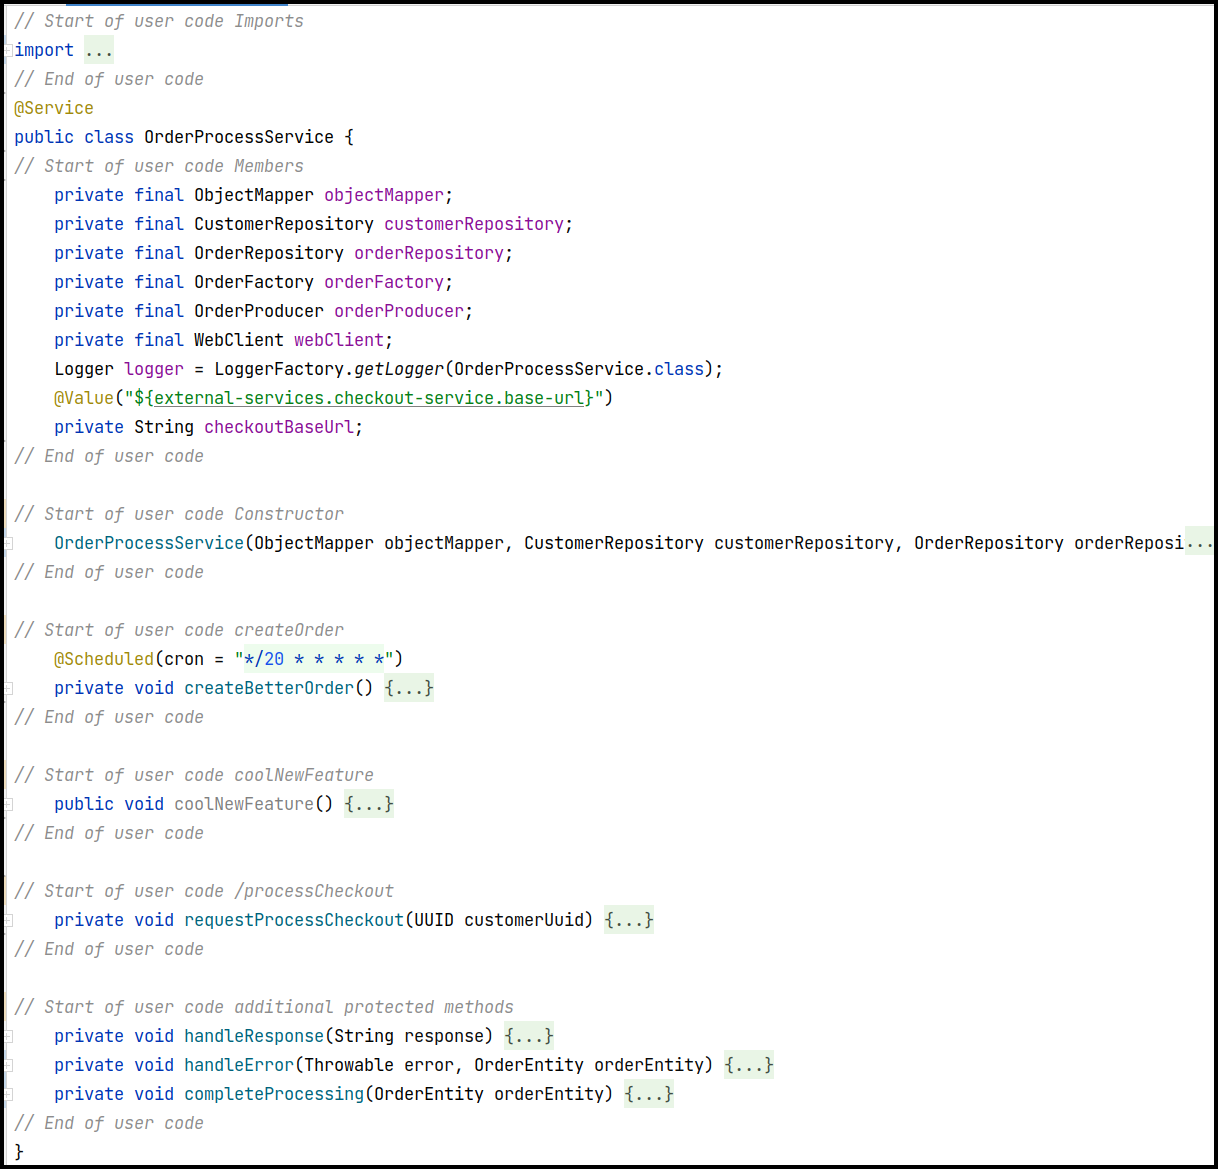
\includegraphics[width=\textwidth]{bilder/gen/1_light.png}
\caption{Generierter Code mit geschützten Bereichen}
\end{figure}

\newpage

Hierbei ist hervorzuheben, dass die Methode \glqq coolNewFeature()\grqq{} erst nach der initialen Codegenerierung dem Modell als Verhalten hinzugefügt wurde. Dabei blieb bestehender Code erhalten. Der durch das Verhalten neu generierte wurde problemlos hinzugefügt.
Das Löschen dieses Verhaltens aus dem Modell führt ebenfalls zu einer funktionierenden Entfernung der Methode und deren Implementierung. Das Umbenennen würde hingegen zum Verlust der Implementierung führen.

Alternativ zu diesem feingranulareren Ansatz ist es auch möglich, ganze Klassen als einen einzigen geschützten Bereich zu kennzeichnen. Exemplarisch wurde dies in einem dem Quellcode anhängenden Beispielprojekt \cite{bspprojekt}, welches einen Microservice enthält, für Entity und Repository umgesetzt. In diesem ist ebenso die in Abbildung 6.1 abgebildete Service-Klasse zu finden.

\subsection{Open Rewrite}

Eine weitere Möglichkeit, solche Migrationen durchzuführen, ist die Verwendung der Software OpenRewrite \cite{rewrite}. Sie kann über eine Gradle- oder Maven-Build-Konfiguration in ein Projekt eingebunden werden und ermöglicht es, bereits existierende Migrationsrezepte zu nutzen. Diese erlauben einfache Refactorings, wie das Umbenennen eines Pakets, einer Methode oder das automatische Formatieren von Code. Auch komplexere Rezepte, die eine Codebasis vollständig auf eine aktuelle Java-Version migrieren können, existieren. Zudem können eigene Rezepte in Java implementiert werden. Ergänzend zur Implementierung mit AQL-geschützten Bereichen sollen nun exemplarisch einige Rezepte vorgestellt werden. Diese wurden ebenfalls dem Beispielprojekt hinzugefügt.

\begin{lstlisting}[caption=OpenRewrite Rezepte]
---
type: specs.openrewrite.org/v1beta/recipe
name: app.ChangeMethod
displayName: Change method name example
recipeList:
  - org.openrewrite.java.ChangeMethodName:
      methodPattern: app..* createOrder()
      newMethodName: createBetterOrder
      
---
type: specs.openrewrite.org/v1beta/recipe
name: app.order
recipeList:
  - org.openrewrite.java.ChangePackage:
      oldPackageName: app.order
      newPackageName: app.ordernew
\end{lstlisting}

In der rewrite.yml werden neue Namen für das Ändern von Methodennamen und das Umstrukturieren von Paketen innerhalb der Rezepte definiert.

\newpage

\begin{lstlisting}[caption=Anwenden von OpenRewrite Rezepten]
rewrite {
    activeRecipe(
            'app.order',
            'app.ChangeMethod',
            'org.openrewrite.java.format.AutoFormat'
    )
}
\end{lstlisting}

In der build.gradle können diese dann mit dem vorher definierten Rezeptnamen referenziert werden. Auch Rezepte wie das automatische Formatieren von Code, die keine weitere Konfiguration verlangen, können hier genutzt werden. Durch das Anwenden des Gradle-Tasks \glqq rewriteRun\grqq{} werden diese nun ausgeführt.

Somit können auch speziellere Migrationen, die sich nicht durch Änderungen des Modells umsetzen lassen, durchgeführt werden.
\chapter{Anwendung}

\section{Modellierung einer Microservice-Architektur für einen Anwendungsfall}

\subsection{Vorstellung des Anwendungsfalles}

In diesem Kapitel wird eine Softwarelösung für einen Webshop modelliert. Diese Lösung soll es Kunden ermöglichen, sich zu registrieren, Bestellungen durchzuführen, diese abzuwickeln und abschließend an ein Backoffice-System zu übertragen. Zusätzlich sollen bei der Registrierung betrügerische Kunden automatisch erkannt werden. Um das Einkaufsverhalten exemplarisch zu zeigen, soll das Kaufverhalten so implementiert werden, dass Kunden so lange Käufe tätigen, bis sie zwei Bestellungen getätigt haben. Weiterhin soll der Checkout-Prozess mit einer fünfprozentigen Wahrscheinlichkeit fehlschlagen. Das Registrieren eines Kunden, die Erzeugung einer Bestellung und der erfolgreiche Checkout-Prozess sollen in Form eines Events prozessiert werden, und dieses soll dem Backoffice-System mitgeteilt werden.

\begin{figure}[ht]
\centering
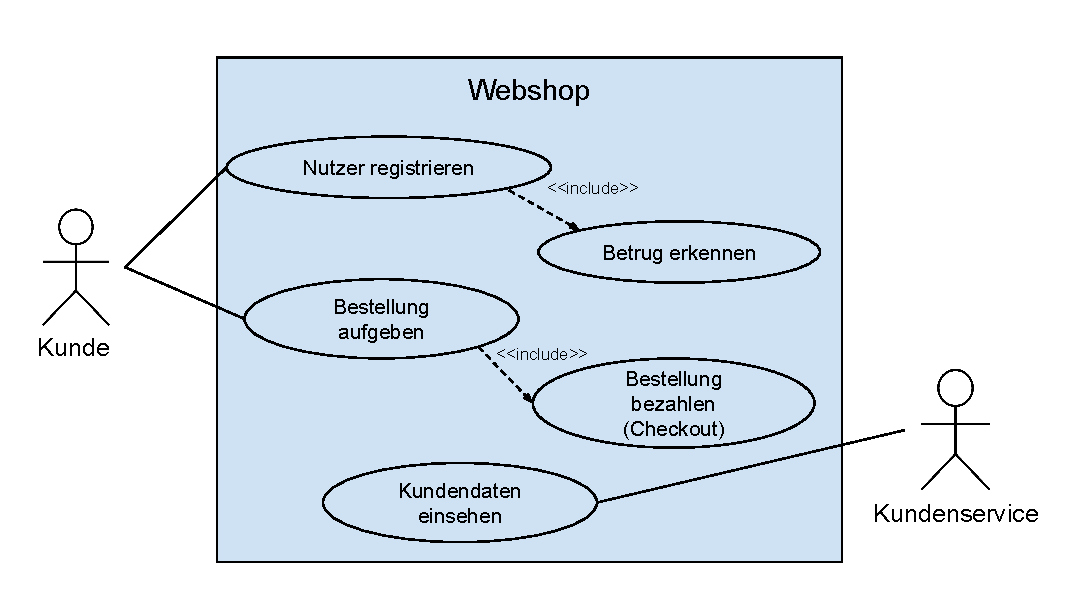
\includegraphics[height=8cm]{bilder/k6/UseCase.pdf}
\caption{Use-Case Diagramm für den Webshop-Anwendungsfall}
\end{figure}

\newpage

\subsection{Ablauf der Modellierung mit Editor}

Nach der Initialisierung des Grundmodells, wie in Kapitel 5.3 definiert, werden mit einer ContextRelationshipDescription erkannte BoundedContexts modelliert. Diesen werden Microservices und DomainModels zugewiesen. Ebenso wird ein SharedKernel \glqq Pricing\grqq{} identifiziert, welcher Teil der Kontexte \glqq Order\grqq{} und \glqq Checkout\grqq{} ist. Eine Abhängigkeit zu einer passenden Bibliothek wird ebenso modelliert. Zusätzlich werden Beziehungen zwischen den BoundedContexts entworfen. Der \glqq Backoffice\grqq-Kontext besitzt als Datensenke ein auf seinen Anwendungszweck als Datenarchiv spezialisiertes Verständnis von Kunden-, Bestellungs- und Checkout-Informationen. Dies kann in der Realität durch ein ERP-System wie SAP oder Salesforce notwendig sein. Der Kundenkontext wird als Published Language gegenüber dem Order Kontext modelliert, was durch das Veröffentlichen einer Beschreibung der Datenstruktur für Kunden umgesetzt werden könnte. Da der Order Kontext aus Gründen der Datensparsamkeit nur ein begrenztes Verständnis von den Daten hat, wird in Form einer Anticorruption Layer der Kunde in ein eigenes Modell übersetzt. Anders hingegen wird der Checkout modelliert, welcher das Modell der Bestellung übernehmen soll.

\begin{figure}[ht]
\centering
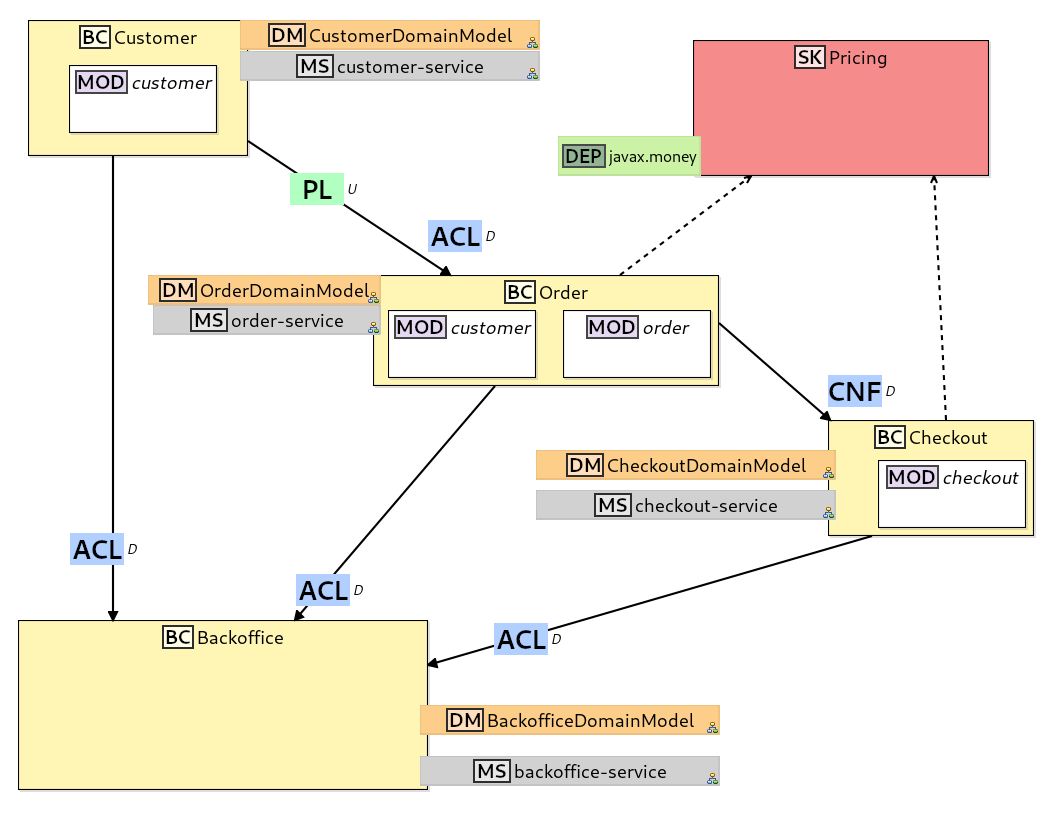
\includegraphics[width=\textwidth]{bilder/k6/1.png}
\caption{Modellierung der Bounded Contexts für den Anwendungsfall}
\end{figure}

\newpage

Nun werden die einzelnen DomainModels weiter verfeinert. Dem DomainModel des BoundedContext Order werden zwei Module, \glqq Customer\grqq{} und \glqq Order\grqq, hinzugefügt. Eine \glqq CustomerEntity\grqq{} beinhaltet die notwendigen Daten eines Kunden und wird von einer \glqq CustomerFactory\grqq{} erzeugt sowie von einem \glqq CustomerRepository\grqq{} persistiert. Dieses kann Kunden mit weniger als einer variablen Anzahl an Bestellungen finden. Ähnlich wird eine \glqq OrderEntity\grqq{} mit einem Repository und einer Factory modelliert, welche bei der Erzeugung einen Bestellwert berechnet. Ein \glqq OrderProcessService\grqq{} erzeugt Bestellungen und fordert einen Checkout-Prozess an. Zusätzlich wird das Event, das bei der Erzeugung einer Bestellung auftritt, angelegt. Das Modellieren anderer Domänen funktioniert nun konzeptionell symetrisch zu diesem Vorgehen.

\begin{figure}[ht]
\centering
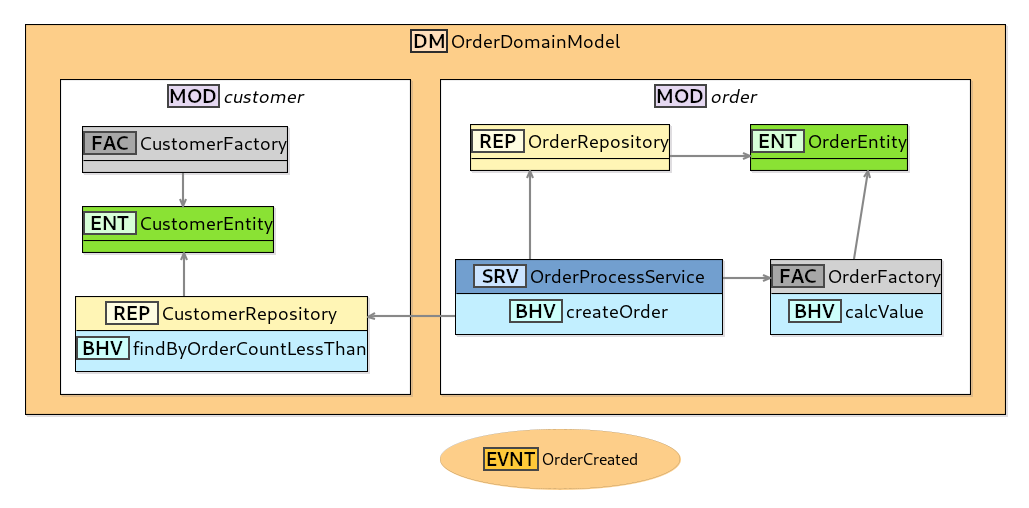
\includegraphics[width=\textwidth]{bilder/k6/3.png}
\caption{Modellierung des OrderDomainModel für den Anwendungsfall}
\end{figure}

\begin{figure}[ht]
\centering
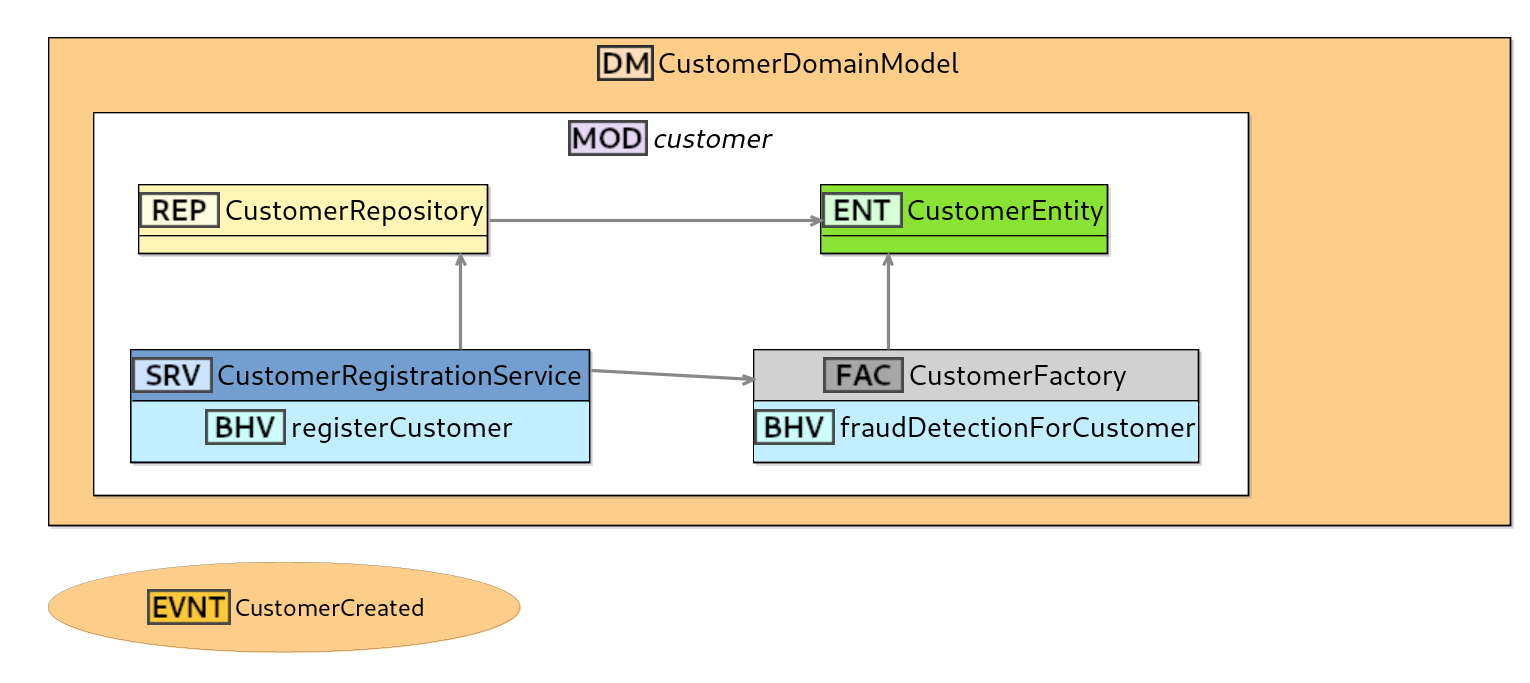
\includegraphics[width=\textwidth]{bilder/k6/extra.png}
\caption{Konzeptionell symetrische Modellierung des CustomerDomainModel}
\end{figure}


\newpage


In der Übersicht über die Microservice-Kommunikation werden nun passende Schnittstellen für die Microservices angelegt. Mittels asynchroner Schnittstellen werden über Topics Daten übertragen. Die Kommunikation zwischen Order und Checkout hingegen läuft synchron, da eine Bestellung erst abgeschlossen wird, sobald ein Checkout erfolgreich durchgeführt wurde.


\begin{figure}[ht]
\centering
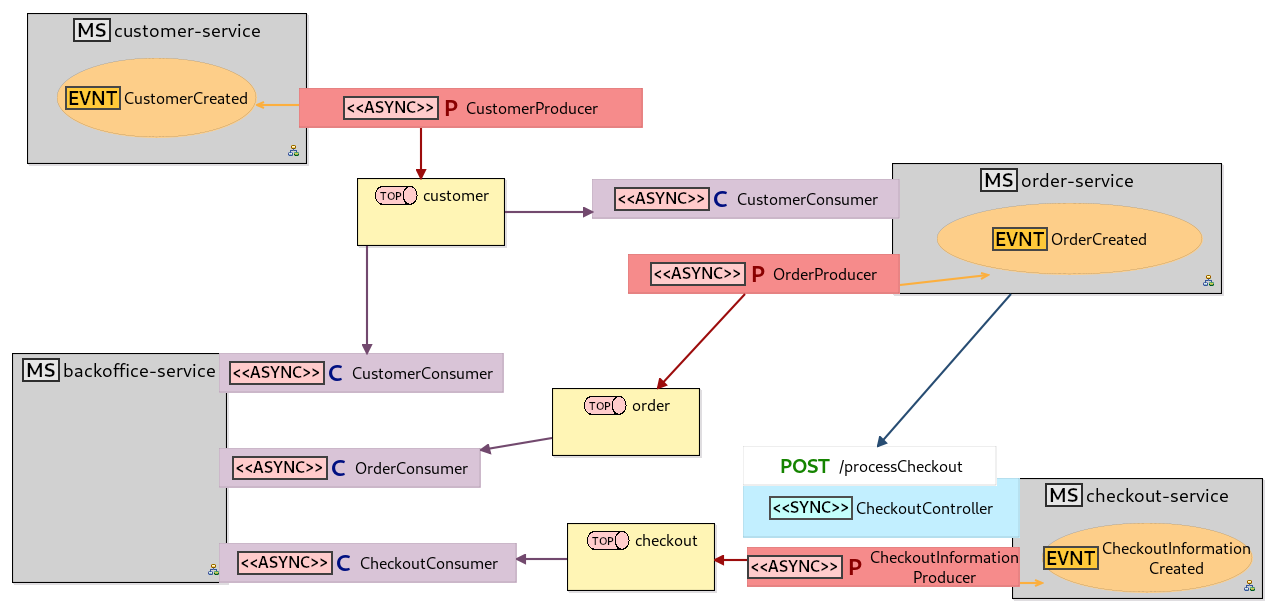
\includegraphics[width=0.95\textwidth]{bilder/k6/4.png}
\caption{Modellierung der Kommunikation zwichen Microservices für den Anwendungsfall}
\end{figure}


In den servicespezifischen Schnittstellenbeschreibungen werden die im vorherigen Modellierungsschritt definierten Schnittstellen den Modellelementen zugewiesen. Hier wird beispielsweise durch den \glqq OrderProcessService\grqq{} der Checkout-Service angefragt und mit dem \glqq OrderProducer\grqq{} das erfolgreiche Erzeugen einer Bestellung auf das im vorherigen Schritt angelegte Topic geschrieben. Weiterhin werden dem \glqq CustomerConsumer\grqq{} die passende Factory zum Erzeugen der Entities und das Repository zum Persistieren zugewiesen.

\begin{figure}[ht]
\centering
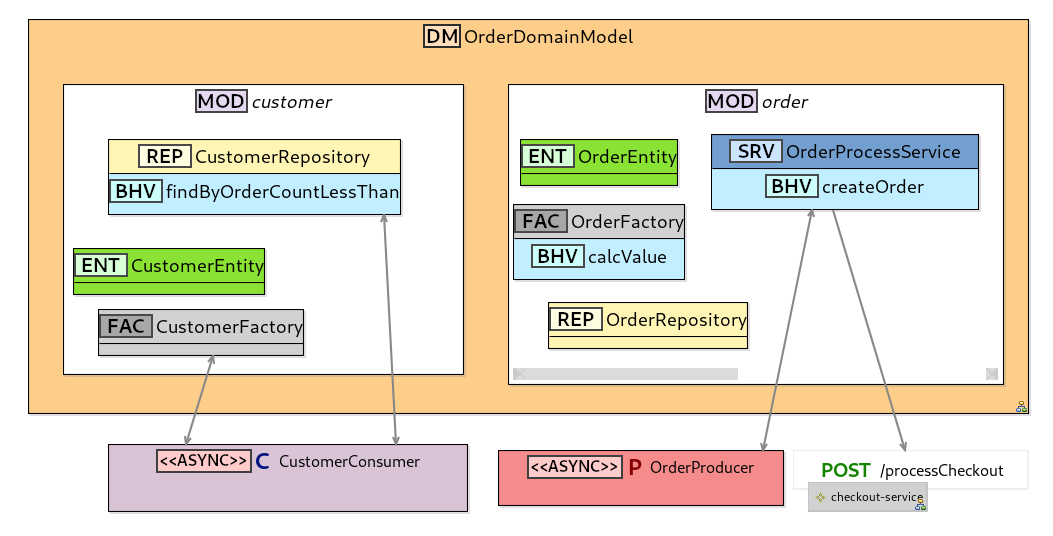
\includegraphics[width=0.95\textwidth]{bilder/k6/5.png}
\caption{Modellierung des Schnittstellen auf Serviceebene für den Anwendungsfall}
\end{figure}

\newpage

Nun kann abschließend der Cloud-Konfiguration ein Cluster hinzugefügt werden, und diesem wiederum je Service ein Deployment. Abschließend werden die Build-Konfigurationen angelegt und diesen die bereits bei der Analyse der Domäne modellierte Bibliothek \glqq javax.money\grqq{} zugewiesen.

\begin{figure}[ht]
\centering
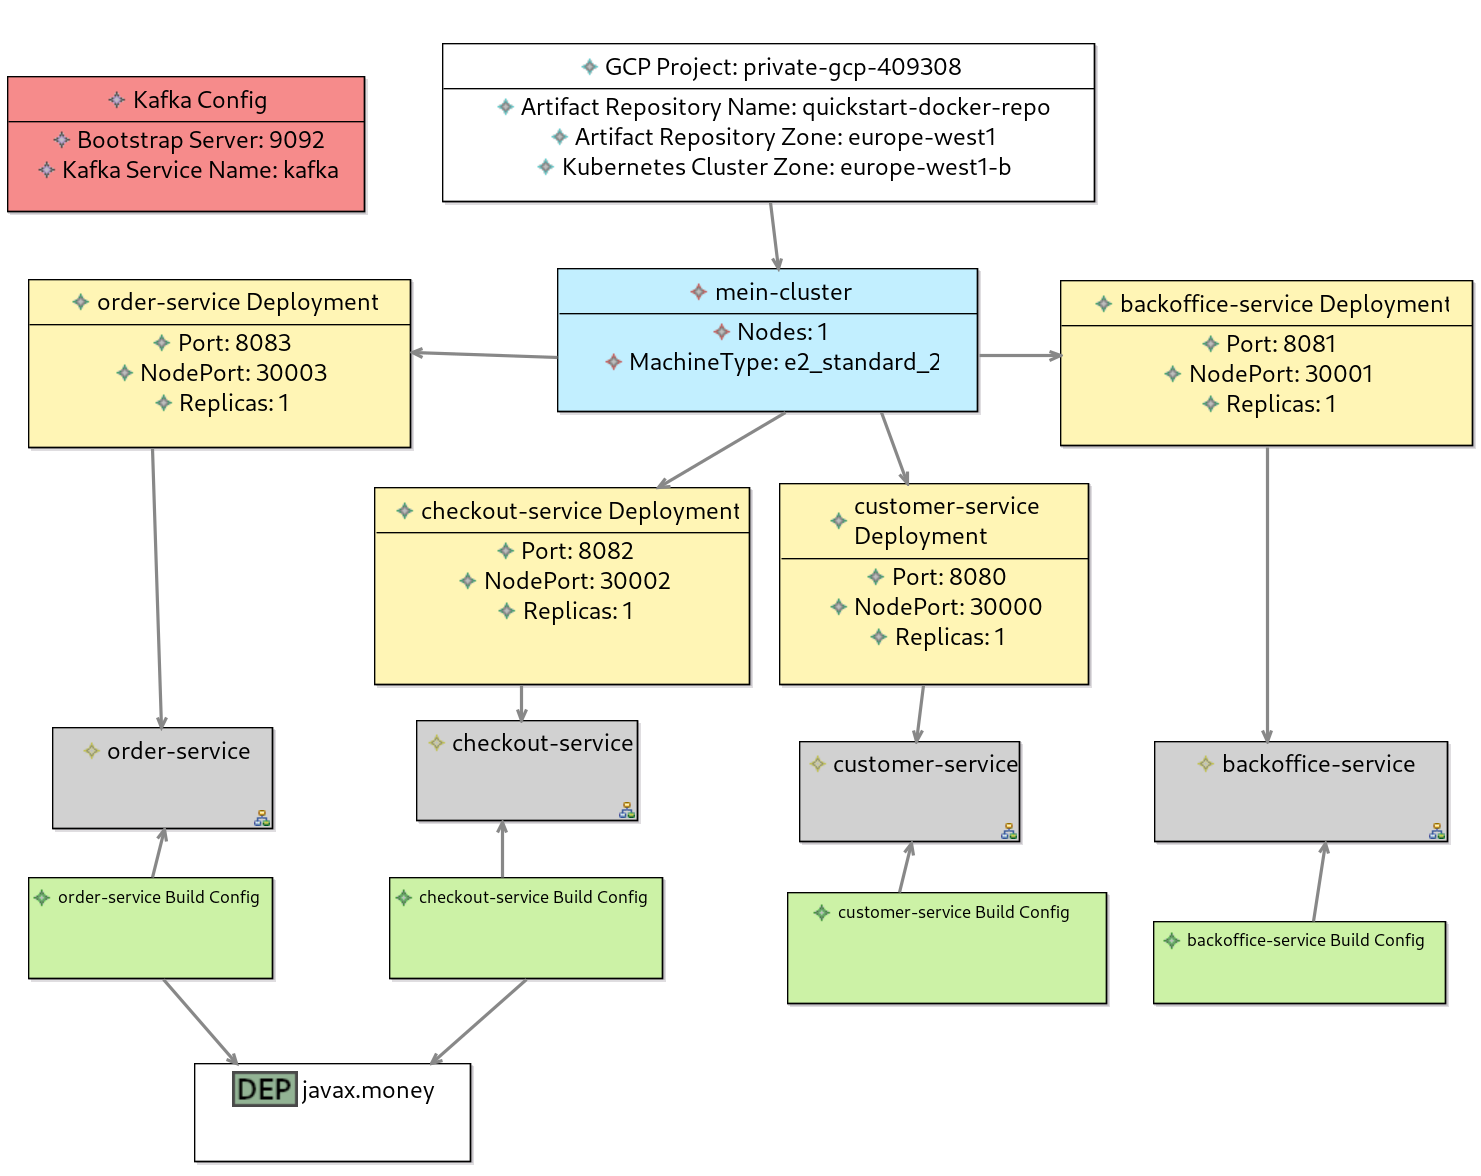
\includegraphics[width=\textwidth]{bilder/k6/6.png}
\caption{Modellierung der Infrastruktur für den Anwendungsfall}
\end{figure}

Somit wurde ein Anwendungsfall mit einer Microservice-Architektur modelliert, die die Konzepte des DDD einbezieht. Weiterhin wurden eine Ausführungsumgebung und die zur Ausführung benötigten Abstraktionen in dieses Architekturmodell einbezogen.

\newpage

\section{Inbetriebnahme}

Mit diesem Modell kann nun der dem Modell entsprechende Code generiert werden. Im Folgenden sollen die abschließenden Schritte beschrieben werden, die nun notwendig sind, um die generierten Projekte in der Cloud auszuführen.

Die modellierten Funktionalitäten müssen zunächst implementiert werden. Dies wird hier exemplarisch anhand der Methode gezeigt, die Bestellungen erzeugt.

\begin{figure}[ht]
\centering
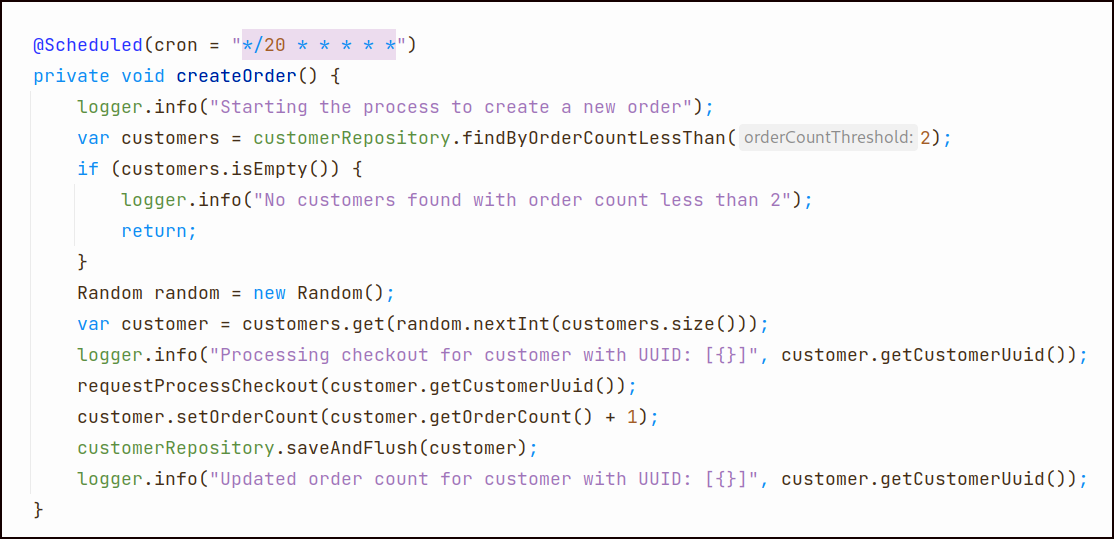
\includegraphics[width=\textwidth]{bilder/k7/1_light.png}
\caption{Implementieren von fehlenden Methoden vor der Inbetriebnahme}
\end{figure}

Weiterhin müssen Klassen attributiert werden. Im Folgenden wird ein Vergleich zwischen einer generierten Entity und einer leicht ausimplementierten Variante gezeigt.

\begin{figure}[ht]
\centering
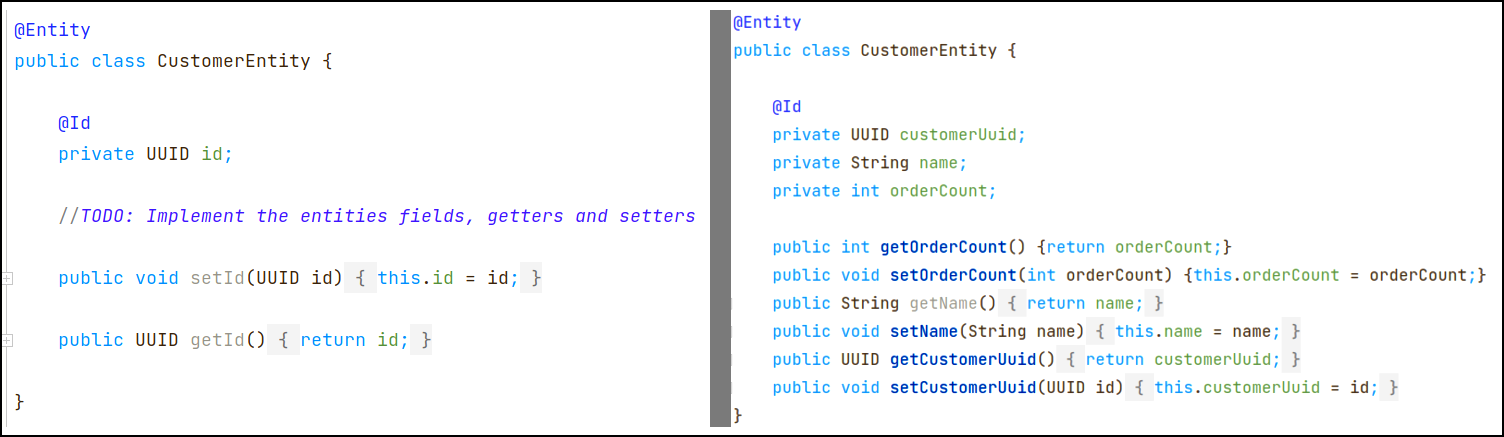
\includegraphics[width=\textwidth]{bilder/k7/2_light.png}
\caption{Implementieren von fehlenden Klassenattributen vor der Inbetriebnahme}
\end{figure}

\newpage

Um das Codegenerierungstemplate lesbar zu gestalten, wurde es durch Verwendung von Tabstopps entsprechend formatiert. Dies führt jedoch zu dem Problem, dass diese mitgeneriert werden, was zu schlecht lesbarem Code führt. Deswegen wird in einem weiteren manuellen Schritt der Code nochmals formatiert. Die folgende Abbildung zeigt exemplarisch die dadurch eingesparte Menge an Codezeilen:

\begin{figure}[ht]
\centering
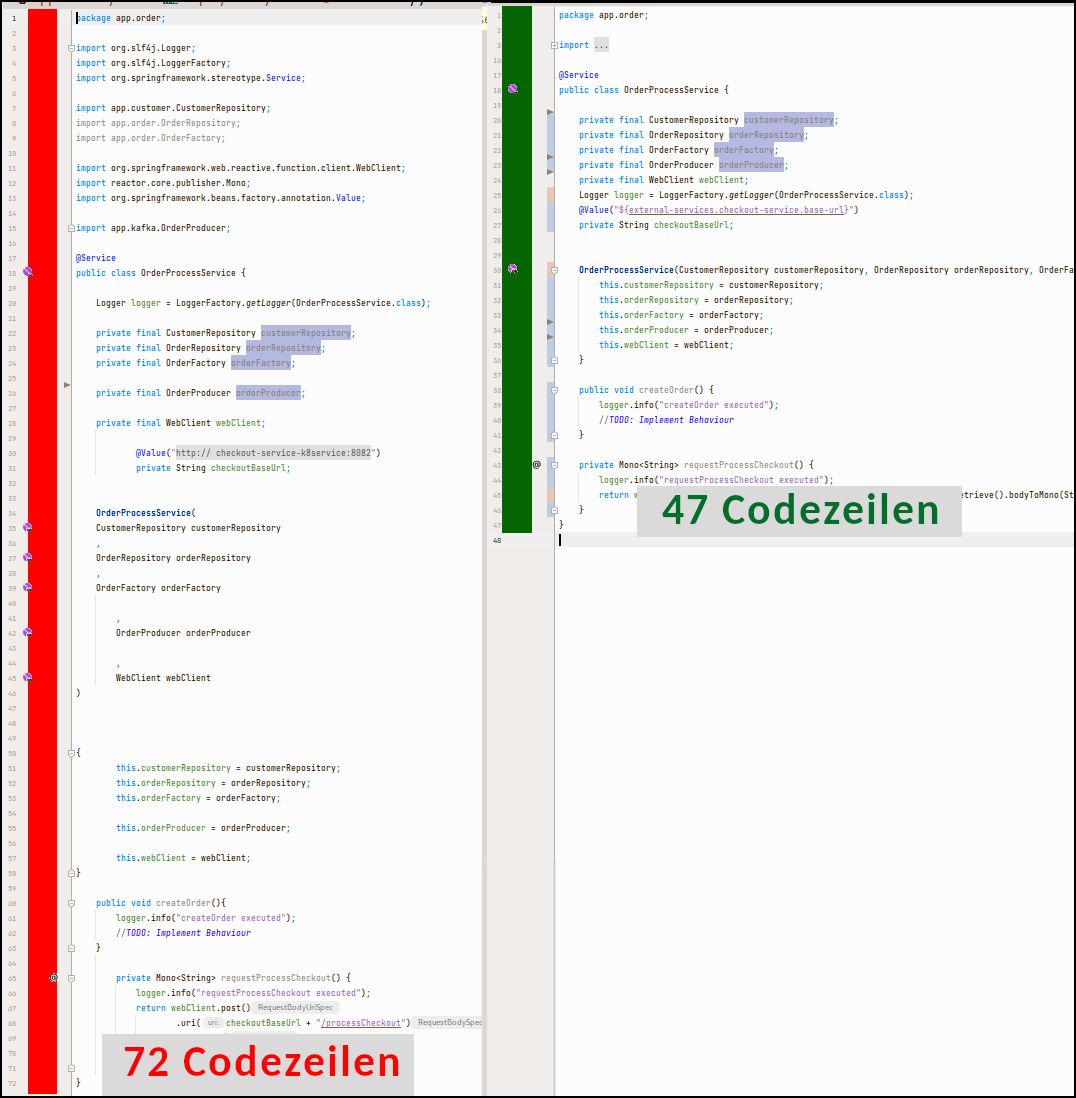
\includegraphics[width=\textwidth]{bilder/k7/3.png}
\caption{Abschließende Code-Formatierung für bessere Lesbarkeit}
\end{figure}

\newpage

Nachdem alle notwendigen Anpassungen durchgeführt wurden, können mit den generierten Bash-Skripten für die Dienste Deployments ausgeführt werden. Zu beachten ist bei den Skripten die möglicherweise notwendige Anpassung des Wurzelverzeichnisses. Dieses sollte auf das Verzeichnis verweisen, welches die generierten Dienste enthält. Durch die folgende Ausführung können dann die Dienste ausgerollt werden.

\begin{table}[h]
\centering
\small
\begin{tabular}{|c|l|}
\hline
\textbf{Schritt} & \textbf{Beschreibung}                                      \\ \hline
1                & Erzeugen von Cluster und Artifact Repository, wenn noch nicht vorhanden.               \\ \hline
2                & Whitelisten der eigenen IP                                 \\ \hline
3                & Deployment des Kafka-Images                                \\ \hline
4                & Erzeugen der Kafka-Topics                                  \\ \hline
5                & Erzeugen der Gradle-Wrapper                                \\ \hline
6                & Bauen der Images                                           \\ \hline
7                & Deployment der Services                                    \\ \hline
\end{tabular}
\caption{Deployment-Schritte für die Software}
\label{tab:deployment_steps}
\end{table}

Damit wäre die modellierte Microservice-Architektur ausgeliefert und kann sowohl über Logs beobachtet, als auch über direkte HTTP-Anfragen angesprochen werden. Somit wurde mittels eines modellgetriebenen Softwareentwicklungsansatzes eine lauffähige Microservice-Architektur modelliert, entwickelt und bereitgestellt.

Der vollständige Quellcode, der das in dieser Arbeit konzipierte Metamodell, die Definition der konkreten Syntax, das Generierungstemplate und verschiedene Beispielprojekte umfasst, liegt dieser Arbeit bei. Weiterhin ist dieser öffentlich in einem GitHub-Repository \cite{github} einsehbar (Stand: 30. Januar 2024).
\chapter{Fazit und Ausblick}

Das entworfene Metamodell für Microservices kann nun genutzt werden, um basierend auf einem modellgetriebenen Entwicklungsansatz Software zu entwickeln. Dadurch wurde die grundlegende Zielsetzung erfolgreich erfüllt. Weiterhin sind diese Anwendungen auch mit relativ geringem Mehraufwand in eine Cloud-Umgebung auslieferbar. Dementsprechend konnte gezeigt werden, dass die einer Microservice-Architektur zugrunde liegende Infrastruktur, in diesem Fall eine Kubernetes-Architektur in der Google Cloud, berücksichtigt werden kann. Es wurde außerdem gezeigt, dass Microservices auch in einem Deployment-fähigen Zustand modellgetrieben entwickelt werden können.

Trotzdem muss berücksichtigt werden, dass einige vereinfachende Annahmen und Architekturentscheidungen zugunsten dieser Ergebnisse getroffen wurden. Einige davon lassen sich dabei durchaus mit den selbst definierten Entscheidungs- und Bewertungskriterien als sinnvoll und nützlich bewerten. So ist die pragmatische Lösung, ein Microservice-Anwendungsimage auf maximal einen Pod laufen zu lassen, eine Vereinfachung, die für das Lösen von Anwendungsfällen hinreichend ist. Auch die sehr einfache Modellierung des Messaging-Systems Kafka hat sich als ausreichend für den erfolgreichen Betrieb einer Microservice-Architektur erwiesen. Kritischer sind Modellierungsentscheidungen wie das Fehlen einer abstrakten Messaging-Konfigurationsklasse oder der Google Cloud-spezifischen Maschinentyp-Modellierung innerhalb der Kubernetes-Konfigurationsklasse einzuordnen.

Der tatsächliche Mehrwert dieser konzeptionell breiten Modellierung kann ebenfalls kritisch hinterfragt werden. Es ist notwendig, jeden einzelnen Service in einer der Generierung folgenden, feineren Implementierung zu vervollständigen. Dann müssen diese über die erzeugten Skripte manuell ausgerollt werden. Es stellt sich die Frage, inwiefern sich der Aufwand durch den generierten Code reduziert bzw. sogar erhöht. Wie würde sich dies bei einer hochskalierenden Anzahl an Diensten entwickeln? Durch die Erfassung von Software-Qualitätsmetriken ließe sich dies beispielsweise messen. Auch die Möglichkeiten von erhöhter Automatisierung, wie beispielsweise das Modellieren von Deployment-Pipelines und Infrastructure as Code, könnten in diesem Zusammenhang vielversprechende Erweiterungen des Metamodells sein.

Weiterhin wurde versucht, die Eigenschaften von Microservice-Architekturen in das Metamodell einfließen zu lassen. So konnte erfolgreich das Konzept des Domain-Driven Designs in ein Metamodell integriert werden. Es zeigt sich, dass die Abstraktion des DDD gut durch eine konkrete Syntax ausgedrückt werden kann. Diese eignet sich insbesondere sehr gut um Problemdomänen zu analysieren. Die direkte Verbindung zu den technischen Microservice-Konzepten vereinfacht daraufhin die ersten Schritte des Grobentwurfs. Insbesondere die Veranschaulichung der verteilten Systemarchitektur und der genutzten Kommunikationskanäle konnte effektiv umgesetzt werden. Weiterhin zeigt sich der Vorteil des Model-Driven Designs, da die Symmetrien zwischen Codebasis und Modell beachtlich sind. Aber auch hier können wieder verschiedene vereinfachende Abstraktionsschritte thematisiert werden. So wurden viele tiefergehende Konzepte, insbesondere aus dem Bereich des Betriebs wie Monitoring oder Metriken, aber auch Aspekte der Datenbankimplementierung, nicht in das Modell integriert. Dies zeigte sich zwar als nicht unmittelbar notwendig, um lauffähige Anwendungen zu entwickeln, die Problemstellungen lösen. Jedoch könnte man auch argumentieren, dass dies Bereiche sind, die zumindest in einem Modell, das Anspruch auf Vollständigkeit erheben würde, notwendig wären.

Bei der Modellierung des Strategic Designs aus dem DDD kann man auch den dadurch entstandenen Mehrwert kritisch diskutieren. So ist im Rahmen der Problemerfassung und -modellierung ein Verständnis und die Visualisierung der unterschiedlichen Kontexte und ihrer Beziehung zueinander sicherlich hilfreich. Aber der effektive Mehrwert bei einer Codegenerierung konnte während der Konzeption nicht festgestellt werden. Dies lag insbesondere an der Entscheidung, die Attributierung der Modellelemente nicht intensiv zu berücksichtigen. Die Fragestellung, ob eine Modellierung des Strategic Designs im Kontext der Codegenerierung gewinnbringend eingesetzt werden kann, bleibt offen.

Auch die Modellierung von Entities, Value Objects und insbesondere Aggregates ist zu hinterfragen. Die modellierten Assoziationen, die diese Klassen besitzen, wurden im Rahmen der Generierung nicht effektiv aufgegriffen. Die Entscheidung die innere Struktur dieser Klassen händisch zu implementieren zeigte sich in der Umsetzung als eingängiger. Weiterhin existieren andere Metamodelle, die sich auf die Modellierung von Datenstrukturen spezialisieren. Diese aufzugreifen, wäre möglicherweise eine bessere Lösung.

Die Entscheidung, das Metamodell in Schichten zu strukturieren, bot zwar den Vorteil einer klaren Grundstruktur. Retrospektiv zeigten sich jedoch auch Schwächen. Anfangs wurden einige konzeptionelle Gemeinsamkeiten bei der initialen Abstraktion auf Basis eines Modells erkannt. Dabei entwickelte sich die anfangs als technische Schicht abstrahierte Ebene jedoch überraschend anders als erwartet. Es zeigte sich, dass eine zwischenzeitliche explizite Modellierung der fachlichen Interpretation des MDD und der zusätzlichen Interpretation auf Implementierungsebene nicht notwendig war. Dies führte dazu, dass eine Schicht entstand, deren konzeptioneller Kern eher die Kommunikation umfasste. Es stellt sich die Frage, welche Schichteneinteilung geeigneter gewesen wäre. Insbesondere könnte eine ergänzende vertikale Schichtbildung, zusätzlich zur bisherigen horizontalen Einteilung in Fachlichkeit, technische Umsetzung und Infrastruktur, sehr aufschlussreich sein. Eine solche Abstraktion, die den einzelnen Bounded Context, dessen Service und dessen Infrastruktur als eine Komponente begreift, sowie eine weitere Abstraktion, die Gruppen solcher Komponenten beschreibt, könnte interessante Ergebnisse liefern.

Durch die konzipierte Codegenerierung wurde demonstriert, dass Microservice-Anwendungen modellgetrieben erstellt werden können, wobei viele Vorteile der modellgetriebenen Softwareentwicklung genutzt werden. Der modellzentrierte Ansatz ermöglicht insbesondere bei umfassenden und grundlegenden Änderungen, die eine große Anzahl an Services betreffen, eine effektive Umsetzung. Dies gilt vor allem, wenn die Entwicklung von Anfang an modellgetrieben erfolgt, da auf diese Weise manuell hinzugefügter Code geschützt werden kann. Allerdings bedarf die konkrete Umsetzung der Generierung einer genaueren Betrachtung. Es bestehen signifikante Abhängigkeiten zwischen der Generierung und dem Metamodell. So hat sich gezeigt, dass die Art und Weise, wie das Spring Framework Objekte instanziiert, in Kombination mit dem konzipierten Metamodell zu äußerst komplexen und kognitiv anspruchsvollen Templates führen kann.

Die Handhabung von Kafka Producern und Consumern mit Spring wirft die Frage auf, ob eine abstrakte bidirektionale Referenz zwischen Modellelementen und Interfaces auf der Generierungsebene passend ist. Dies liegt an der Dependency Injection, die dazu führt, dass Modellelemente eine klar gerichtete Assoziation zu Produzenten und eine Assoziation zu ihnen von Konsumenten haben. Hier wäre es interessant herauszufinden, wie eine Generierung auf Basis dieses Metamodells mit einer anderen Implementierungstechnologie umgesetzt werden würde. Auch könnte man retrospektiv fordern, dass die Modellierung darauf verzichtet, technologieunabhängige Dienste zu generieren. Dafür würde man die technologiespezifischen Besonderheiten, zum Beispiel die eines Spring Frameworks, bei der Abstraktion berücksichtigen.

Im speziellen Kontext von Migrationen wurde einerseits gezeigt, wie Refaktorisierungen mit diesem Metamodell prinzipiell umgesetzt werden können. Hierbei liegen die Stärken insbesondere in der Veränderung der Grundstruktur von Anwendungen. So lassen sich beispielsweise Änderungen, die sich in Konfigurationsdateien oder Java-Klassen durch das Hinzufügen bzw. Entfernen bestehenden Codes realisieren lassen, gut in einem modellgetriebenen Ansatz umsetzen. Schwieriger gestaltet sich dies bei Änderungen, die bereits feinimplementierten Quellcode betreffen. Hierfür können zwar existierende Technologien wie OpenRewrite integriert werden, jedoch ist eine Nutzung dieser auch unabhängig von einem modellgetriebenen Einsatz denkbar.

Es kann auch notwendig sein, eine Migration einer noch höheren Größenordnung durchzuführen, wie etwa wenn eine Anwendung auf eine völlig neue Technologie umgestellt werden soll. Dabei bringt der modellgetriebene Ansatz, insbesondere zur initialen Codegenerierung, einige interessante Aspekte mit sich, da vor allem das fachliche Modell erhalten bleibt. Auch hier wären Erkenntnisse durch ergänzende Konzepte, die dieses Modell mit einer anderen Zieltechnologie umsetzen, nützlich.

Zusammenfassend lässt sich festhalten, dass das in dieser Arbeit konzipierte Modell für Anwendungen in einem überschaubaren Rahmen solide Ergebnisse liefert, aber die inhaltliche Tiefe von Microservice-Architekturen, der Betrieb dieser in verschiedenen Cloud-Umgebungen und die Fragestellung der effektiven Nutzung für Migrationen nur angeschnitten werden konnten. Zukünftige wissenschaftliche Arbeiten könnten an diesen Ansätzen anknüpfen und auf den in dieser Arbeit gewonnenen Erkenntnissen und Ideen für eine potenziell effektivere Modellierung und Generierung aufbauen.

% Literaturverzeichniss
\newpage
\bibliographystyle{alpha}
\bibliography{bibs/litDB}

\end{document}